\documentclass[pdftex,12pt,a4paper]{report}

\usepackage[portuguese,english]{babel}
\usepackage[T1]{fontenc} 
\usepackage[utf8]{inputenc}
\usepackage[pdftex]{graphicx}
\usepackage{minitoc}
\usepackage{hyperref}
\usepackage{indentfirst}
\usepackage[compact]{titlesec}
\usepackage{fancyhdr}
\usepackage{caption}
\usepackage{pgfplots}
\usepackage{pgfplotstable}
\usepackage{fixltx2e}
\usepackage{mathtools}
\pagestyle{fancy}
\fancyhead{}
\renewcommand*\thesection{\thechapter\arabic{section}}
\newcommand{\HRule}{\rule{\linewidth}{0.5mm}}
\begin{document}

\begin{titlepage}

\begin{center}


\includegraphics[width=0.15\textwidth]{./logo}\\[0.5cm]    

\textsc{\large Universidade de Aveiro \\[1cm]\large departamento de electrónica, telecomunicações e informática}\\[1cm]

\textsc{\large{41541}\large - Sistemas Electrónicos \\[1cm]}

\HRule \\[0.5cm]
{ \huge \bfseries Relatório Trabalho Prático Nº2}\\[0.4cm]
\HRule \\[1cm]

\textsc{\small{8240 - MESTRADO INTEGRADO EM ENGENHARIA DE COMPUTADORES E TELEMÁTICA}}\\[1cm]

\begin{minipage}{0.4\textwidth}

\begin{flushleft} \large
\href{mailto:rafael.ferreira@ua.pt}{António Rafael da \\ Costa Ferreira }
 \small{\\NMec: 67405 | P3}
\end{flushleft}
\end{minipage}
\begin{minipage}{0.4\textwidth}

\begin{flushright} \large
\href{mailto:rodrigocunha@ua.pt}{Rodrigo Lopes \\ da Cunha}
\small{\\NMec: 67800 | P3}
\end{flushright}
\end{minipage}\\[1cm]

{\large Docente:  João Pedro Estima de Oliveira  }\\[0.5cm]

\vfill

{\large Maio de 2014 \\ 2013-2014}

\end{center}

\end{titlepage} %Titulo do Relatorio
\renewcommand{\headrulewidth}{0pt}

%Parte do resumo!
\vspace*{\fill}
\textbf{Introdução:}
\begingroup
Neste trabalho 2 pretende-se estudar as características e utilizações das portas lógicas NMOS, PMOS, CMOS e do BJT e de um díodo.
\endgroup
\vspace*{\fill}
%Parte do resumo!
\newpage

%Renomear Comandos
\renewcommand*\contentsname{Conteúdos}
\renewcommand*\figurename{Figura}
\renewcommand*\tablename{Tabela}

%Conteúdos, dar paragrafo
\tableofcontents
%Headers
\renewcommand{\headrulewidth}{0.15pt}
\lhead{Relatório Trabalho Prático Nº2}
\renewcommand{\thechapter}{}

\clearpage

\section{Parte I - Análise de Circuitos com Díodos}
\begin{figure}[h]
\centerline{\fbox{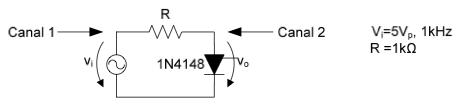
\includegraphics[width=0.5\textwidth]{./Imagens/Diodo-1parte.png}}}
\caption{Circuito com díodo para determinar a característica i-v}\label{diodo_parte1}
\end{figure}

\subsection{Característica i-v de um díodo}
\hbox{\emph{\textbf{Pergunta 1:}}\newline\newline}

Para calcular a característica i-v de um díodo, usando os valores obtidos no osciloscópio e a fórmula $i = \frac{V\textsubscript{i}-V\textsubscript{0}}{R}$ (A) obtemos a seguinte tabela e gráfico:\newline

\minipage{0.65\textwidth}
\begin{tikzpicture}
\begin{axis}[
    title={Gráfico da característica i-v de um díodo},
    xlabel={$v_0$ (V)},
    ylabel={i (mA)},
    xmin=-6, xmax=3,
    ymin=0, ymax=5,
    xtick={-5, -4, -2, 0, 2, 4},
    ytick={-5, -3, 0, 3, 5, 6},
    legend pos=north west,
    ymajorgrids=true,
    grid style=dashed,
]
\addplot table [y=i, x=$v_0$, color=blue, mark=square]{./diodos_data.dat};
\legend{i/v}
\end{axis}
\end{tikzpicture}
\endminipage\hfill
\minipage{0.3\textwidth}
\pgfplotstabletypeset{./diodos_data.dat}
\endminipage\hfill

\begin{figure}[h]
\centerline{\fbox{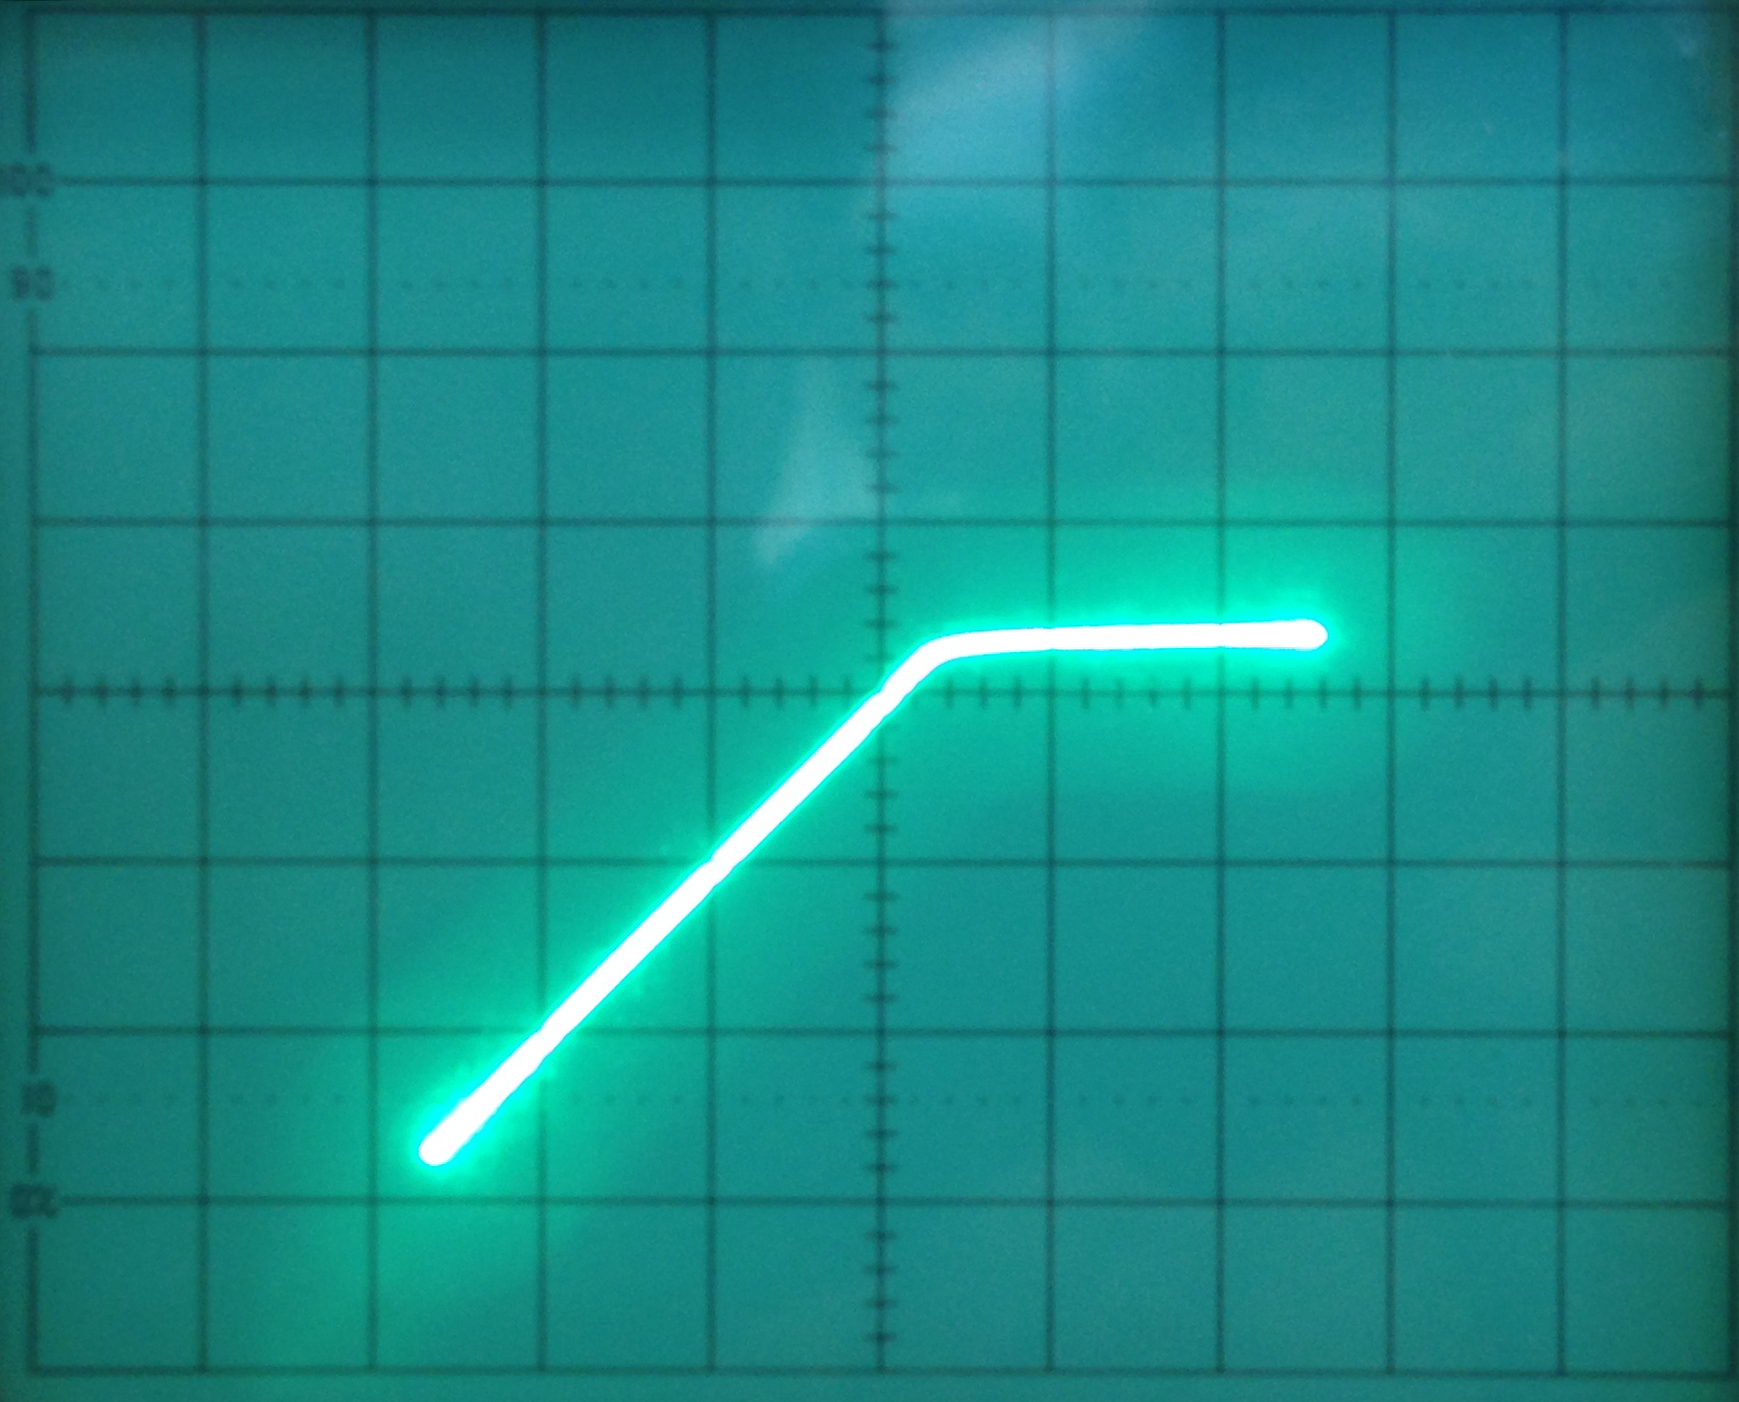
\includegraphics[width=0.35\textwidth]{./Imagens/tp2parte1c.JPG}}}
\caption{Modo \textit{xy} observado no osciloscópio (2V/div) ambos}\label{grafico_1c_osciloscopio}
\end{figure}

Este resultado aproxima-se do esperado, tendo em conta erros de precisão do material usado e de leitura.

\subsection{Formas de onda de V\textsubscript{in}(t)  e V\textsubscript{out}(t) quando a amplitude de V\textsubscript{in}(t) = 0.2V e de V\textsubscript{in}(t) = 2V}
\hbox{\emph{\textbf{Pergunta 2:}}\newline}
As duas ondas sinusoidais coincidem, pois 0,2V não é suficiente para fazer o díodo conduzir, por isso a tensão do canal 2 é igual à do canal 1:

\begin{figure}[h]
\centerline{\fbox{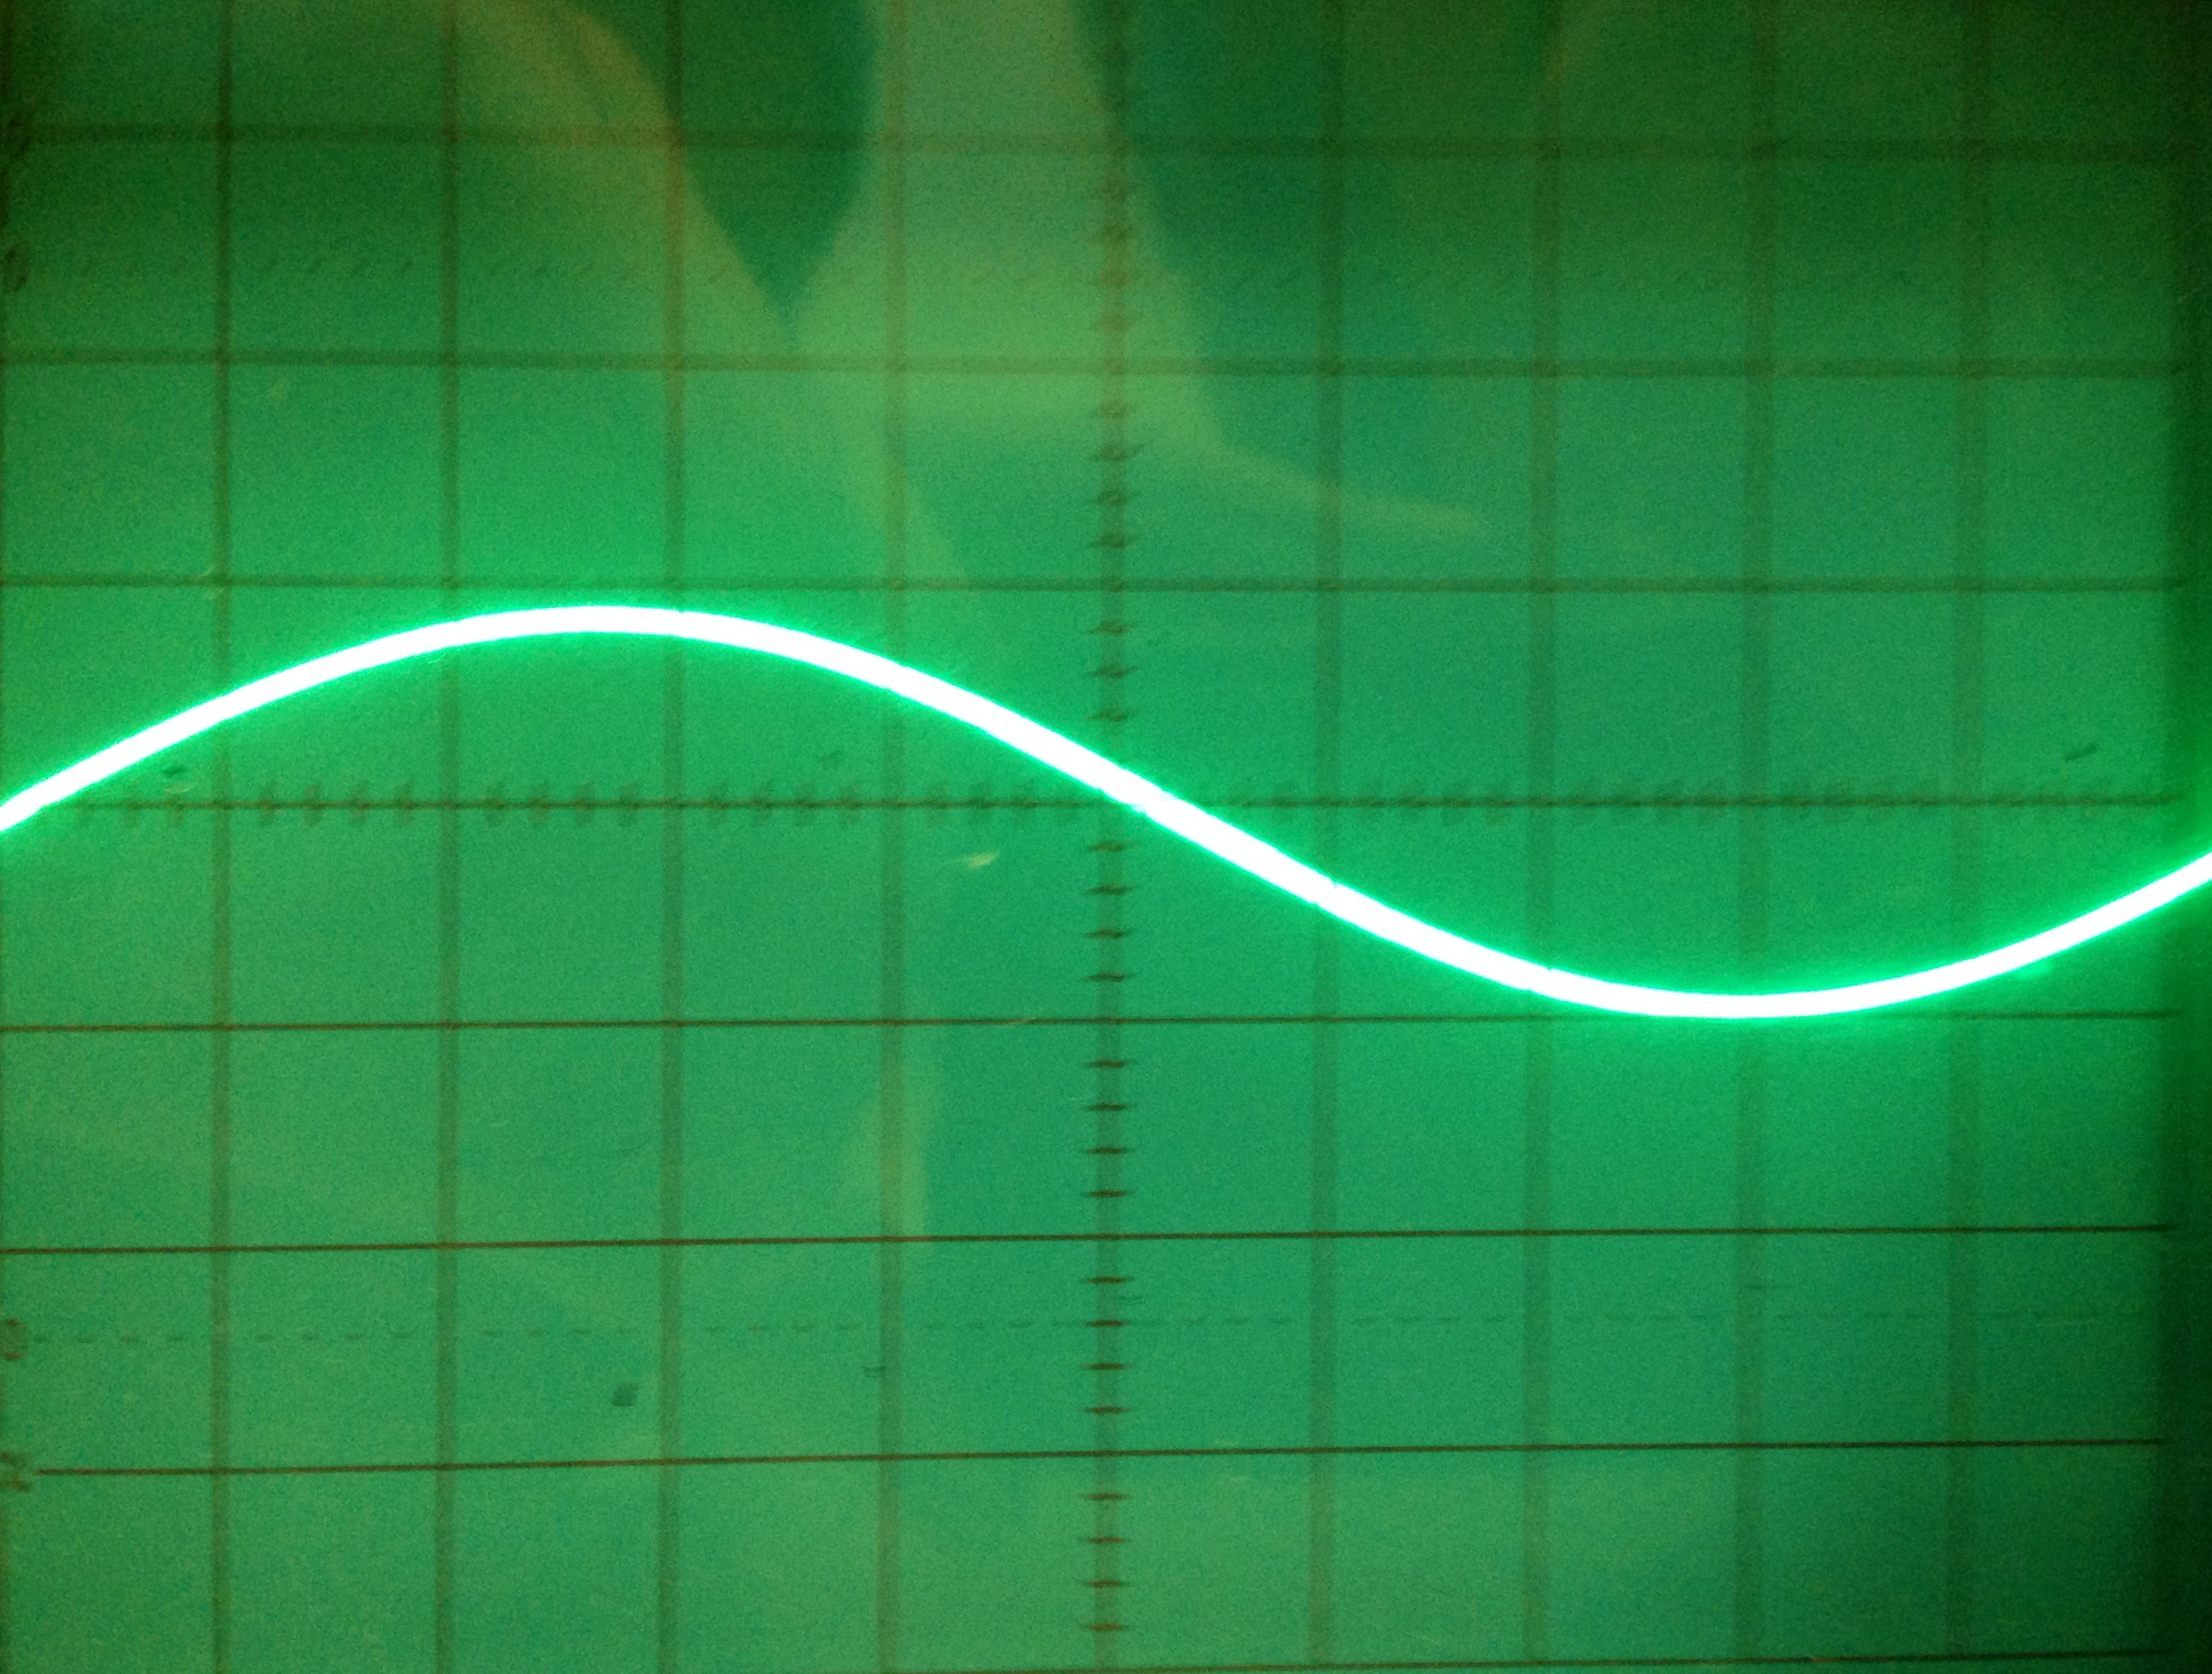
\includegraphics[width=0.5\textwidth]{./Imagens/parte1_ex2_02v_1.jpg}}}
\caption{Vertical: 0,1V/div (ambos); Horizontal: 0,1ms/div (Time A)}\label{grafico_12_02_osciloscopio}
\end{figure}

O díodo limita a tensão do canal 2 para 0,7V (tal como determinado na pergunta 1), sendo a tensão no canal 1 de 2V. Podemos verificar este feito na imagem seguinte:

\begin{figure}[h]
\centerline{\fbox{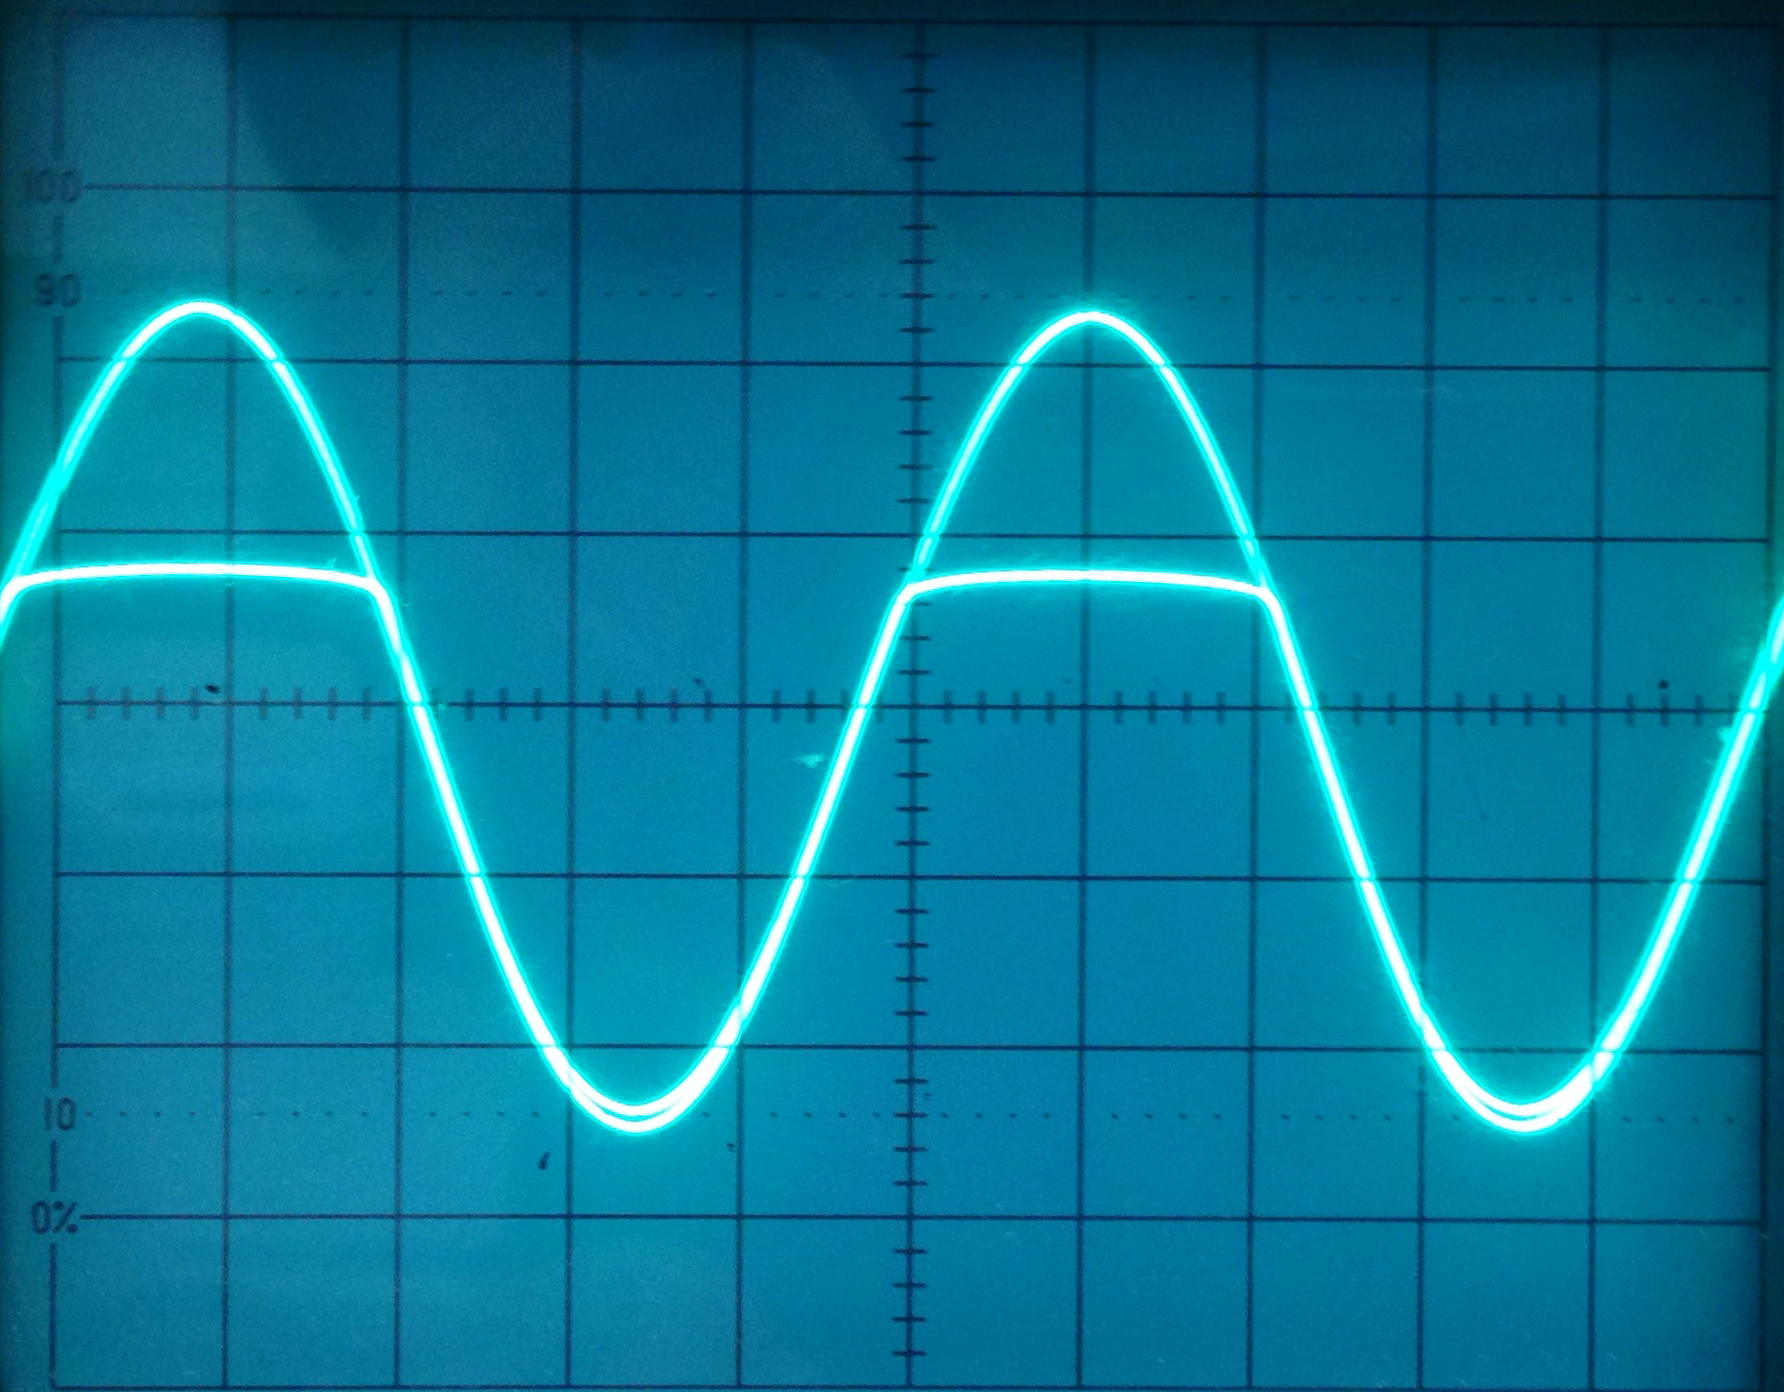
\includegraphics[width=0.5\textwidth]{./Imagens/parte1_ex2_2v_1.jpg}}}
\caption{Vertical: 1V/div (ambos); Horizontal: 0,1ms/div (Time A)}\label{grafico_12_02_osciloscopio}
\end{figure}

\newpage
\subsection{Circuitos limitadores com díodos}
\begin{figure}[h]
\centerline{\fbox{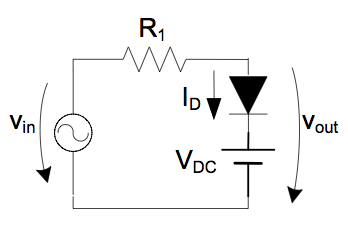
\includegraphics[width=0.35\textwidth]{./Imagens/parte1_ex3.png}}}
\caption{$V_{in}$=10V, 1kHz}\label{circuito13}
\end{figure}

\hbox{\emph{\textbf{Pergunta 3:}\newline}}


Através da expressão $V = R \times I_D$ obtém-se o valor de $R_1$:\newline
\centerline{$I_D = \frac{V_{in} - V_{out}}{R_1} \Leftrightarrow 10^-3 = \frac{10-1,8}{R_1} \Leftrightarrow R_1 = \frac{8,2}{10^-3} \simeq 8,2k\Omega$}\\
\vspace{0.1cm}

Para obter o valor de $V_{DC}$, basta utilizar a expressão $V_{out} = V_D + V_{DC}$:
\centerline{$ 1,8 = 0,6 + V_{DC} \Leftrightarrow V_{DC} = 1,2V$}
\vspace{0.2cm}

Como podemos verificar na imagem abaixo, o circuito ficou limitado a 1,8 V como era pretendido:

\begin{figure}[h]
\centerline{\fbox{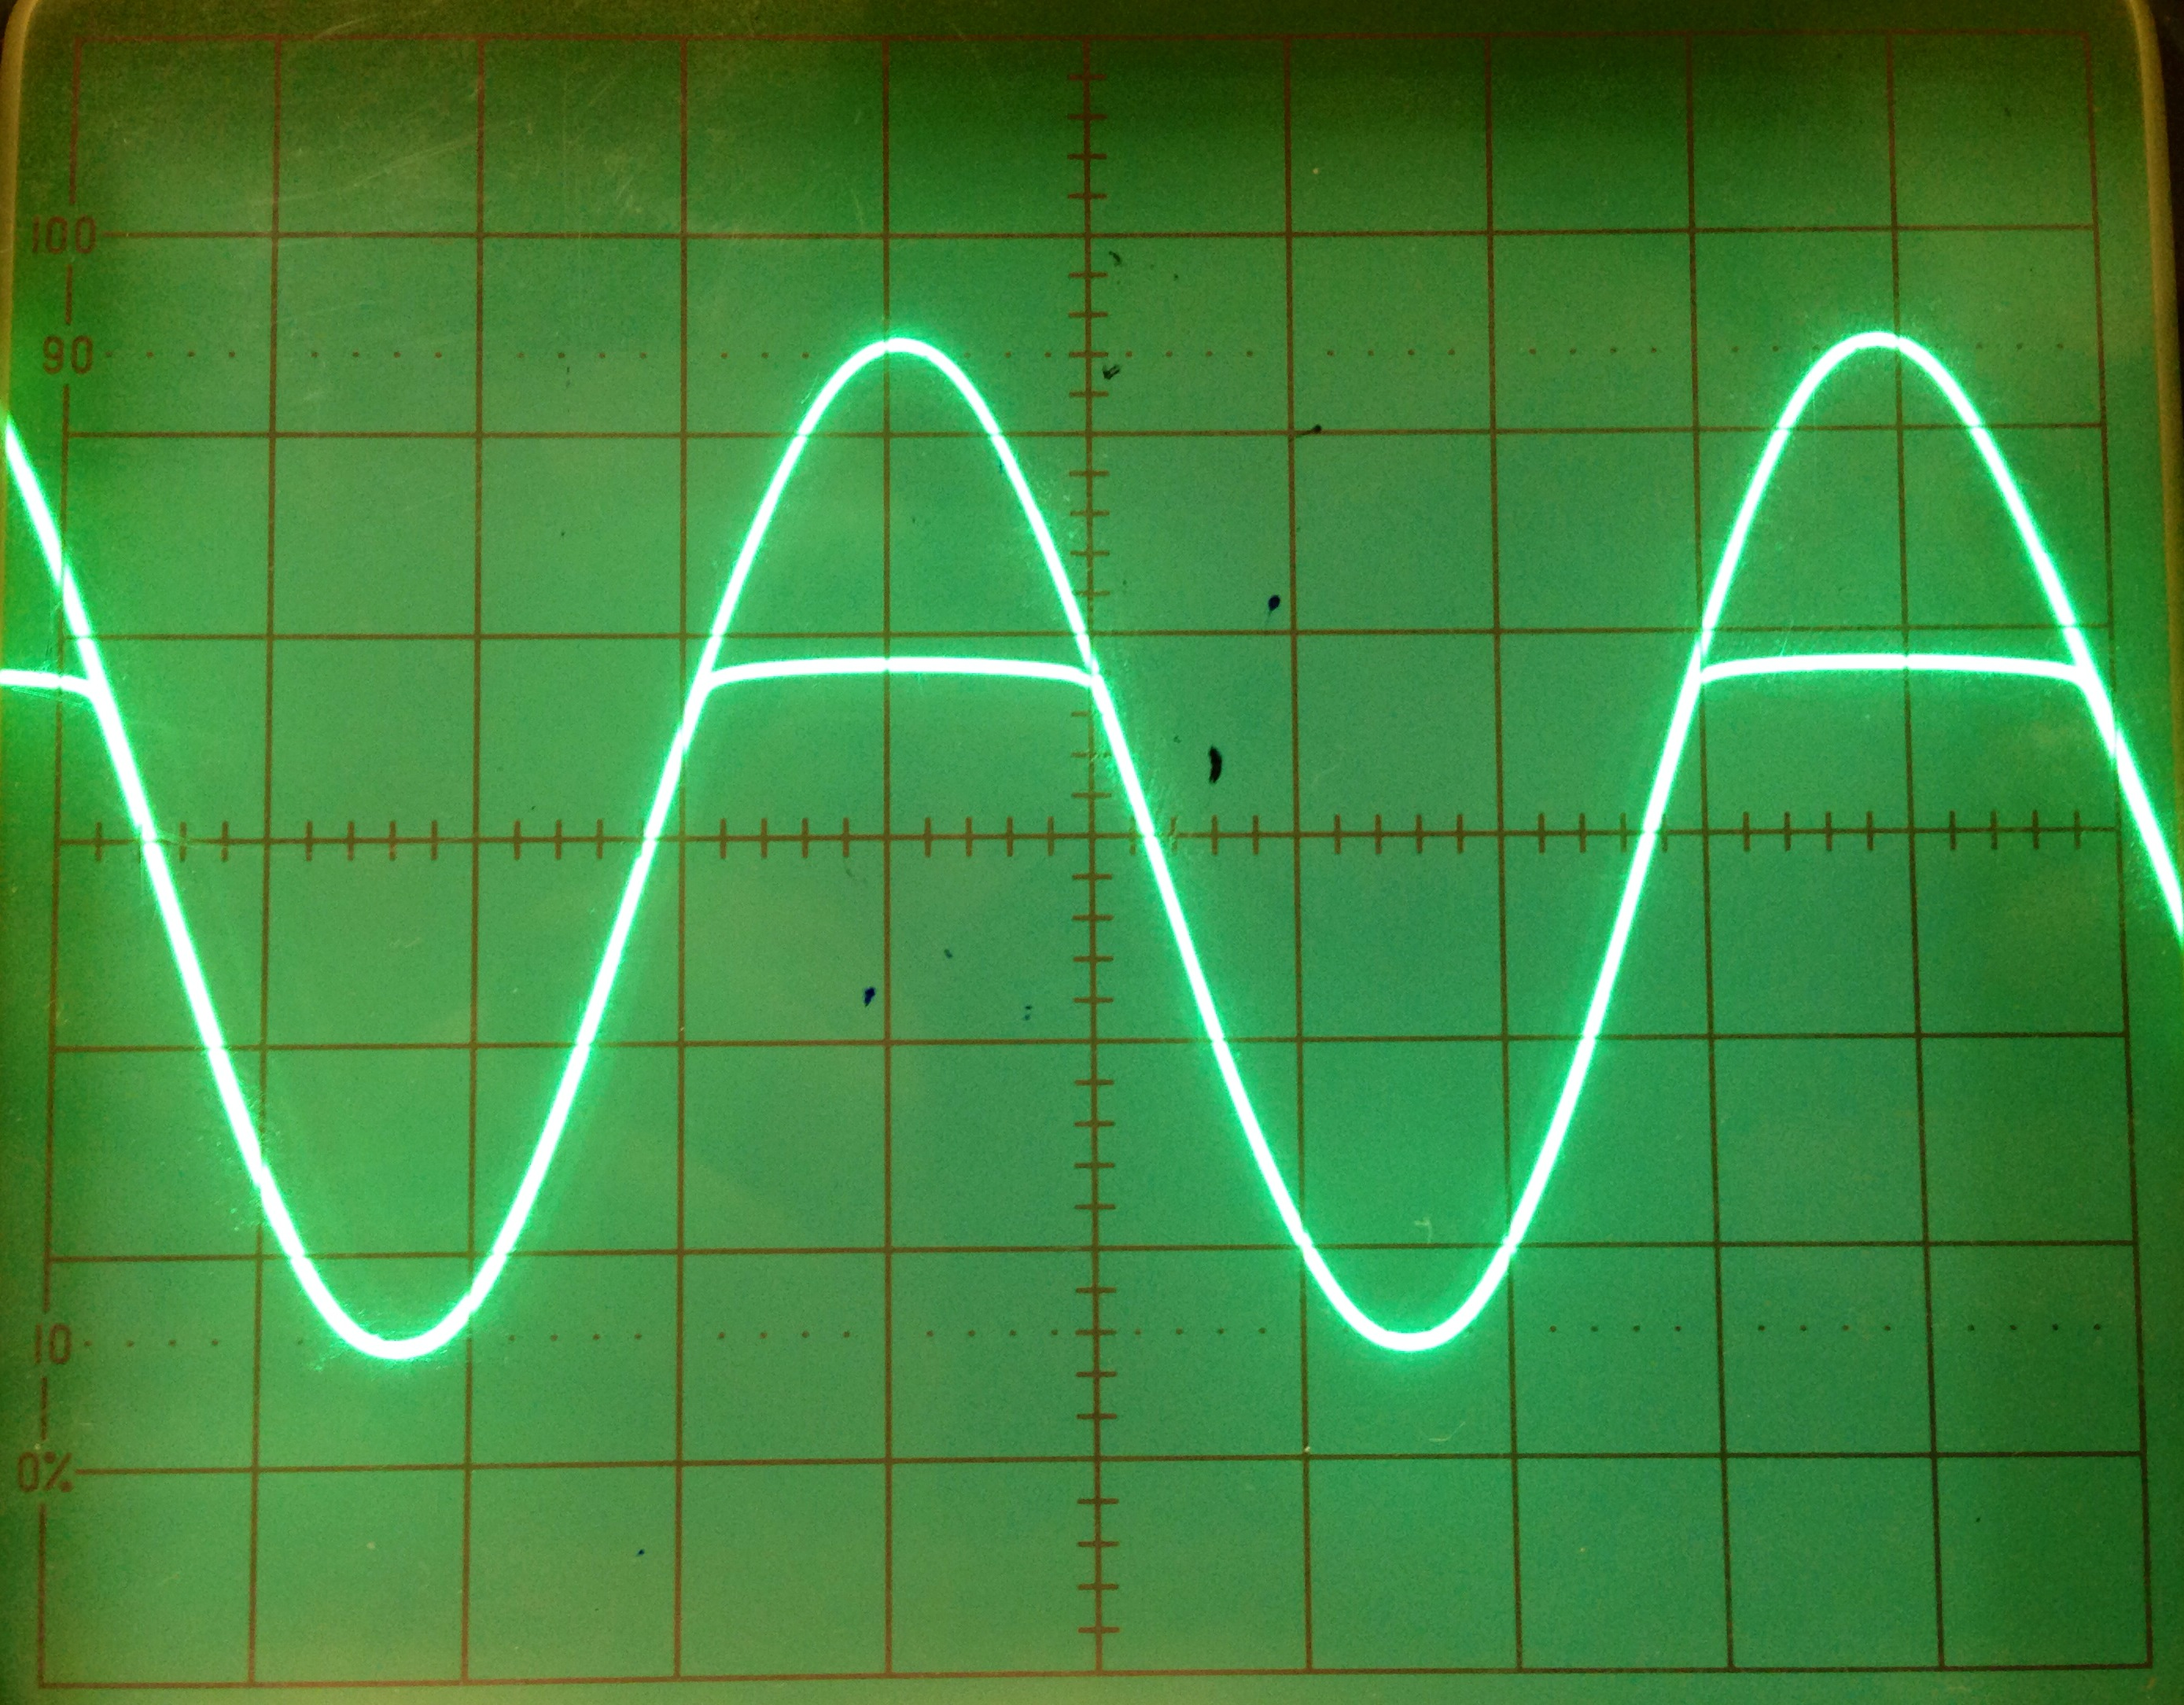
\includegraphics[width=0.55\textwidth]{./Imagens/parte1_ex3_novo.jpg}}}
\caption{Vertical: 2V/div (ambos); Horizontal: 0,2ms/div (Time A)}\label{grafico_1c_osciloscopio}
\end{figure}

\newpage

\section{Parte II - Análise	de	Portas	Lógicas	e	Circuitos	Lógicos}

\begin{figure}[!htb]
\minipage{0.2\textwidth}
  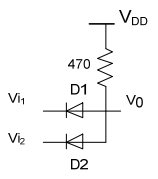
\includegraphics[width=\linewidth]{Imagens/Diodos.png}
  \caption{\\Díodo}\label{fig:fig_diodo}
\endminipage\hfill
\minipage{0.2\textwidth}
  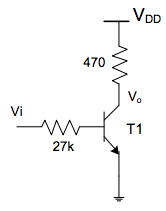
\includegraphics[width=\linewidth]{Imagens/BJT.png}
  \caption{\\BJT}\label{fig:fig_bjt}
\endminipage\hfill
\minipage{0.2\textwidth}
  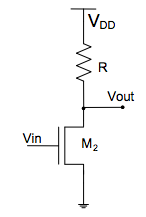
\includegraphics[width=\linewidth]{Imagens/NMOS.png}
  \caption{\\NMOS}\label{fig:fig_nmos}
\endminipage
\minipage{0.2\textwidth}
  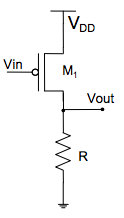
\includegraphics[width=\linewidth]{Imagens/PMOS.png}
  \caption{\\PMOS}\label{fig:fig_pmos}
\endminipage\hfill
\minipage{0.2\textwidth}
  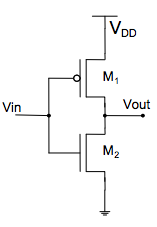
\includegraphics[width=\linewidth]{Imagens/CMOS.png}
  \caption{\\CMOS}\label{fig:fig_cmos}
\endminipage\hfill
\end{figure}

\subsection{Função lógica implementada pelos circuitos anteriores}
A função implementada pelo díodo é um AND.

\begin{table}[h]
\centerline{
\begin{tabular}{|l|l|l|}
\hline
$Vi_1$ & $Vi_2$ & $V_0$ \\ \hline
0 & 0 & 0 \\ \hline
0 & 1 & 0 \\ \hline
1 & 0 & 0 \\ \hline
1 & 1 & 1  \\ \hline
\end{tabular}}
\caption{\\Função lógica do Díodo (AND)}\label{fig:fig_diodo}
\end{table}

Se as duas entradas estiverem a 0, a corrente vai fluir através de ambos os díodos, ficando $V_0$ a  0V.

Para ambas as entradas a 1, a corrente não flui porque o díodo fica em corte, então $V_0$ $\simeq$ $V_{DD}$, ou seja, 1 lógico.

Se uma das entradas estiver a 0, a corrente vai fluir através dela baixando a tensão $V_0$ para o valor da queda nesse díodo.



\newpage

\begin{figure}[h]
  \centerline{\fbox{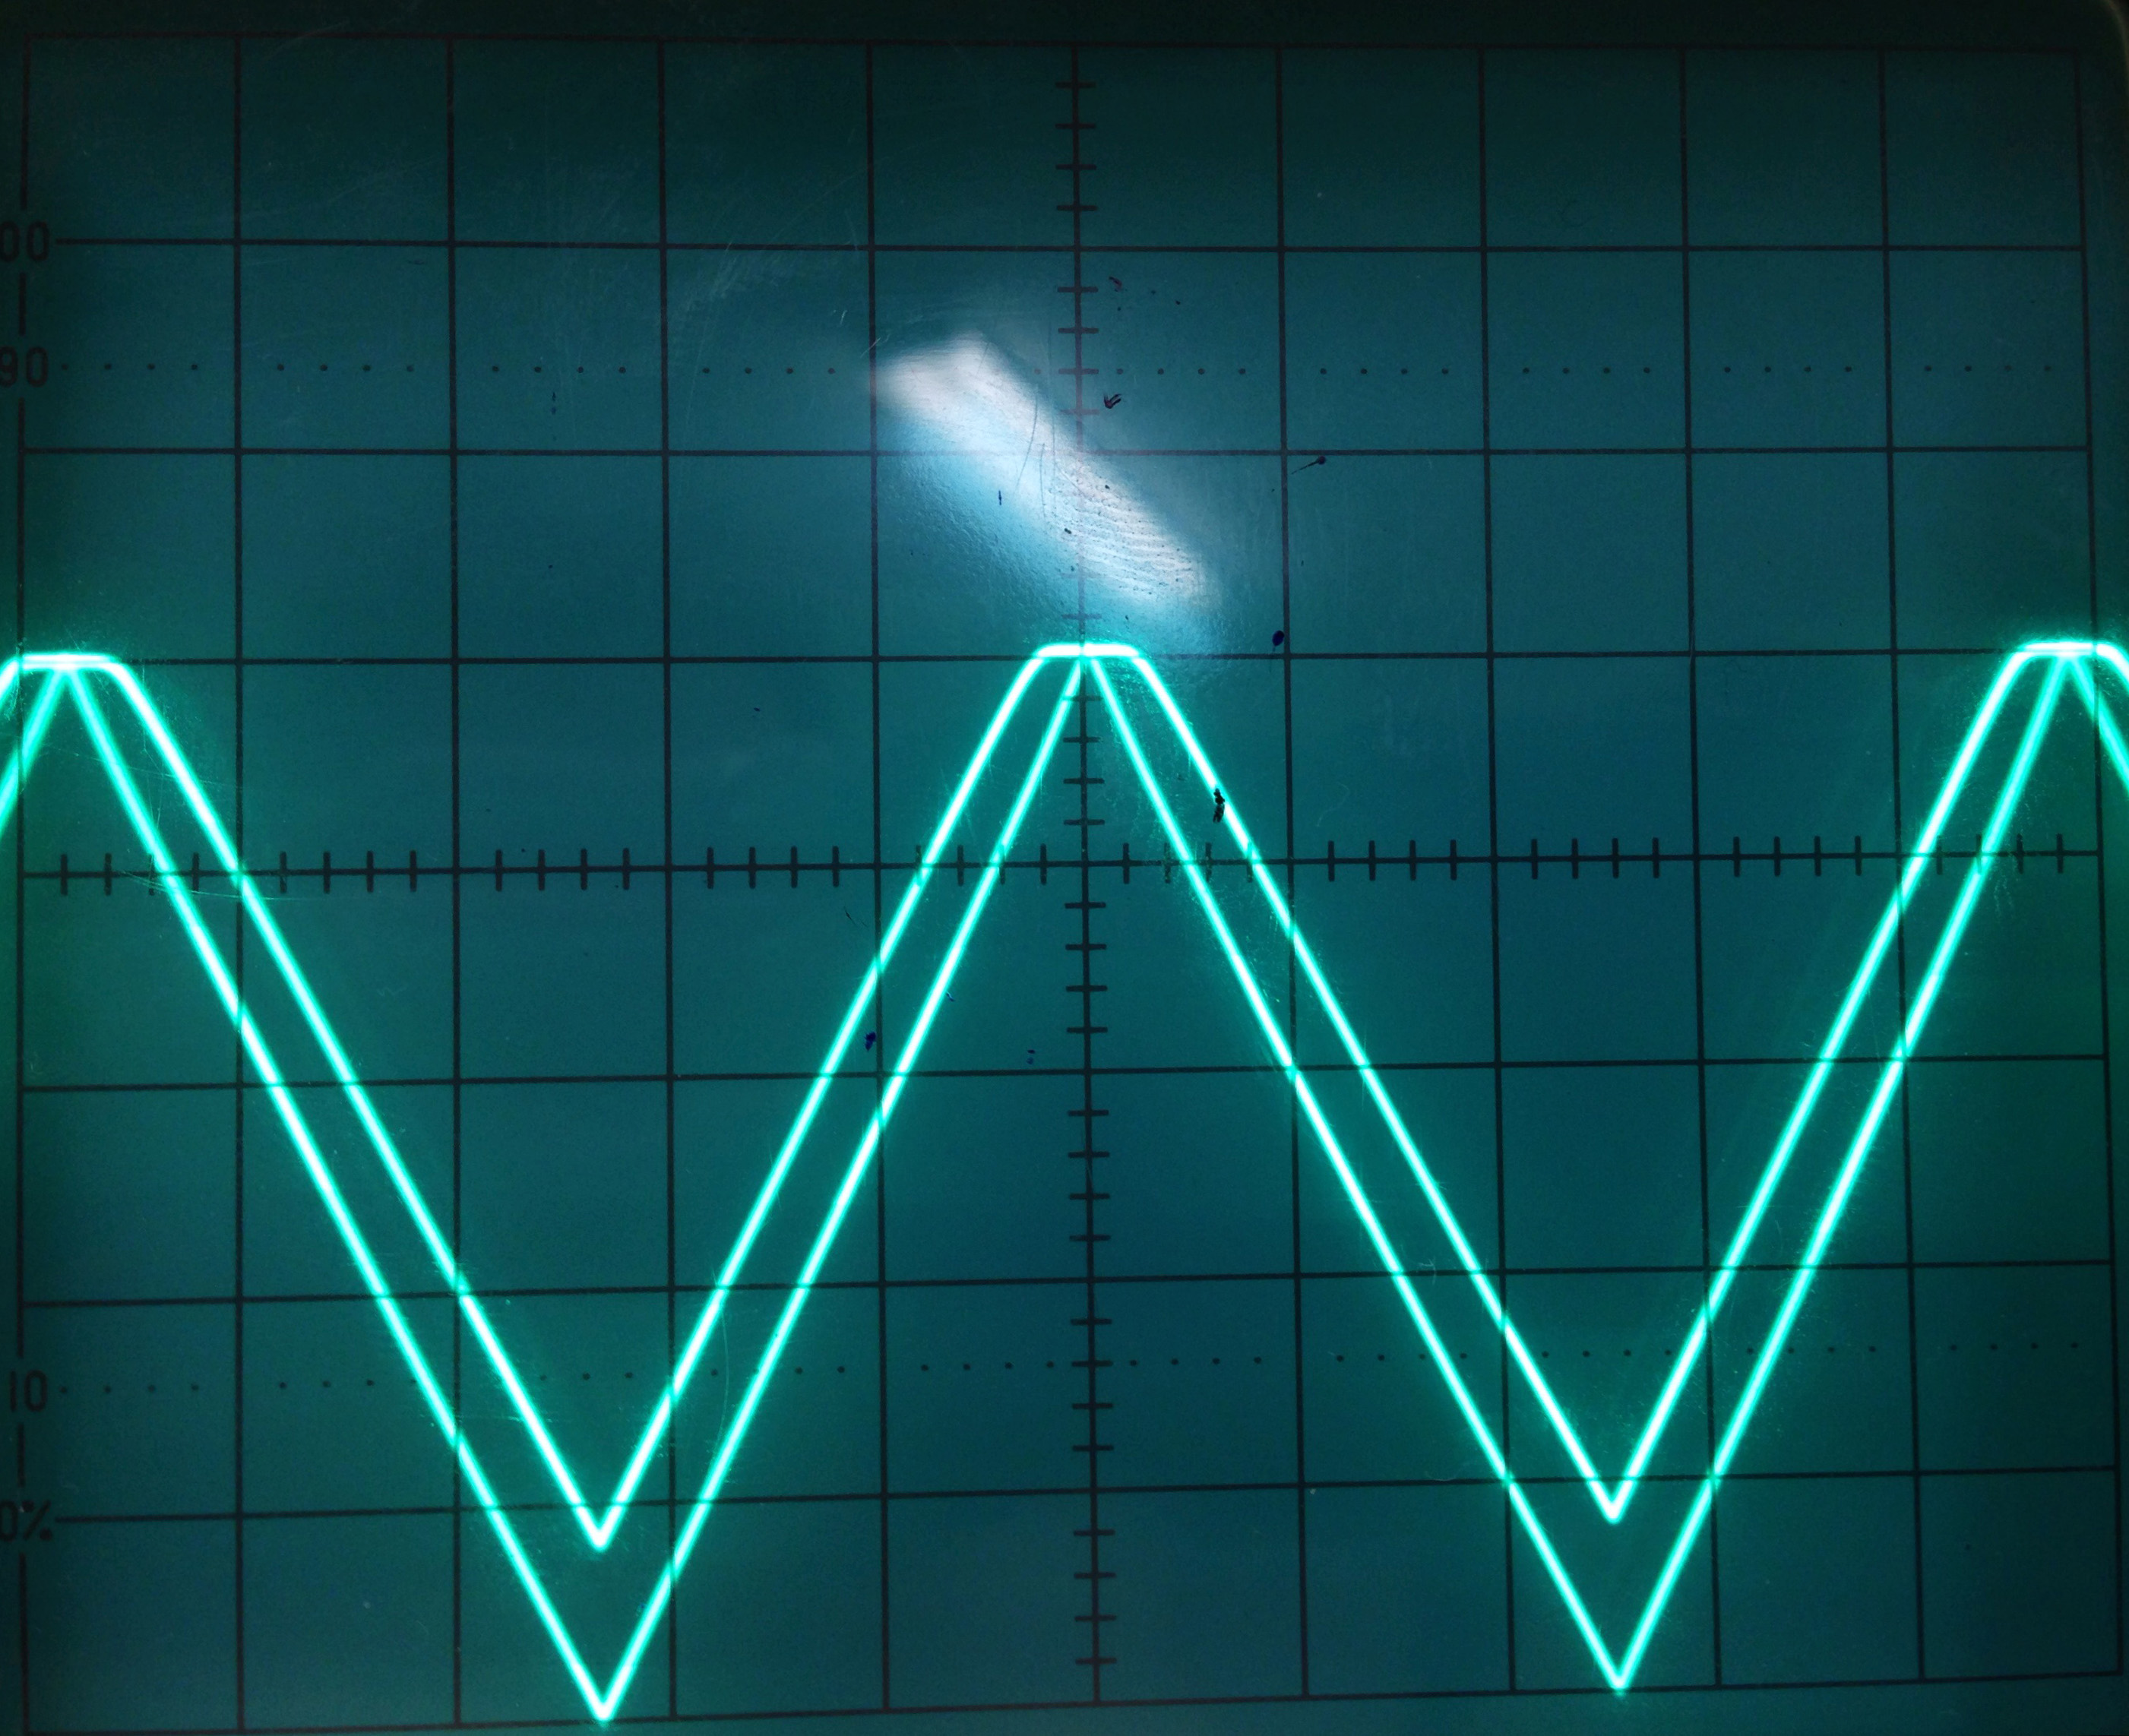
\includegraphics[width=0.4\textwidth]{./Imagens/diodo_2_grafico.jpg}}}
  \caption{\\Vertical: 1V/div (ambos); Horizontal: 0,1ms/div (Time A)}\label{cmos}
\end{figure}

A função lógica implementada pelos quatro circuitos (BJT, NMOS, PMOS e CMOS) é um NOT.

\begin{table}[h]
\centerline{
\begin{tabular}{|l|l|l|}
\hline
$V_{in}$ & $V_{out}$ \\ \hline
0 & 1 \\ \hline
1 & 0 \\ \hline
\end{tabular}}
\caption{\\Função lógica do BJT, \\NMOS, PMOS e CMOS (NOT)}\label{fig:fig_diodo}
\end{table}

No caso do BJT e NMOS quando $V_i$/$V_{in}$ é 1 lógico (+5V), há queda de tensão de $V_{DD}$ para a terra, ficando 0V em $V_0$.

\begin{figure}[!htb]
\minipage{0.5\textwidth}
  \centerline{\fbox{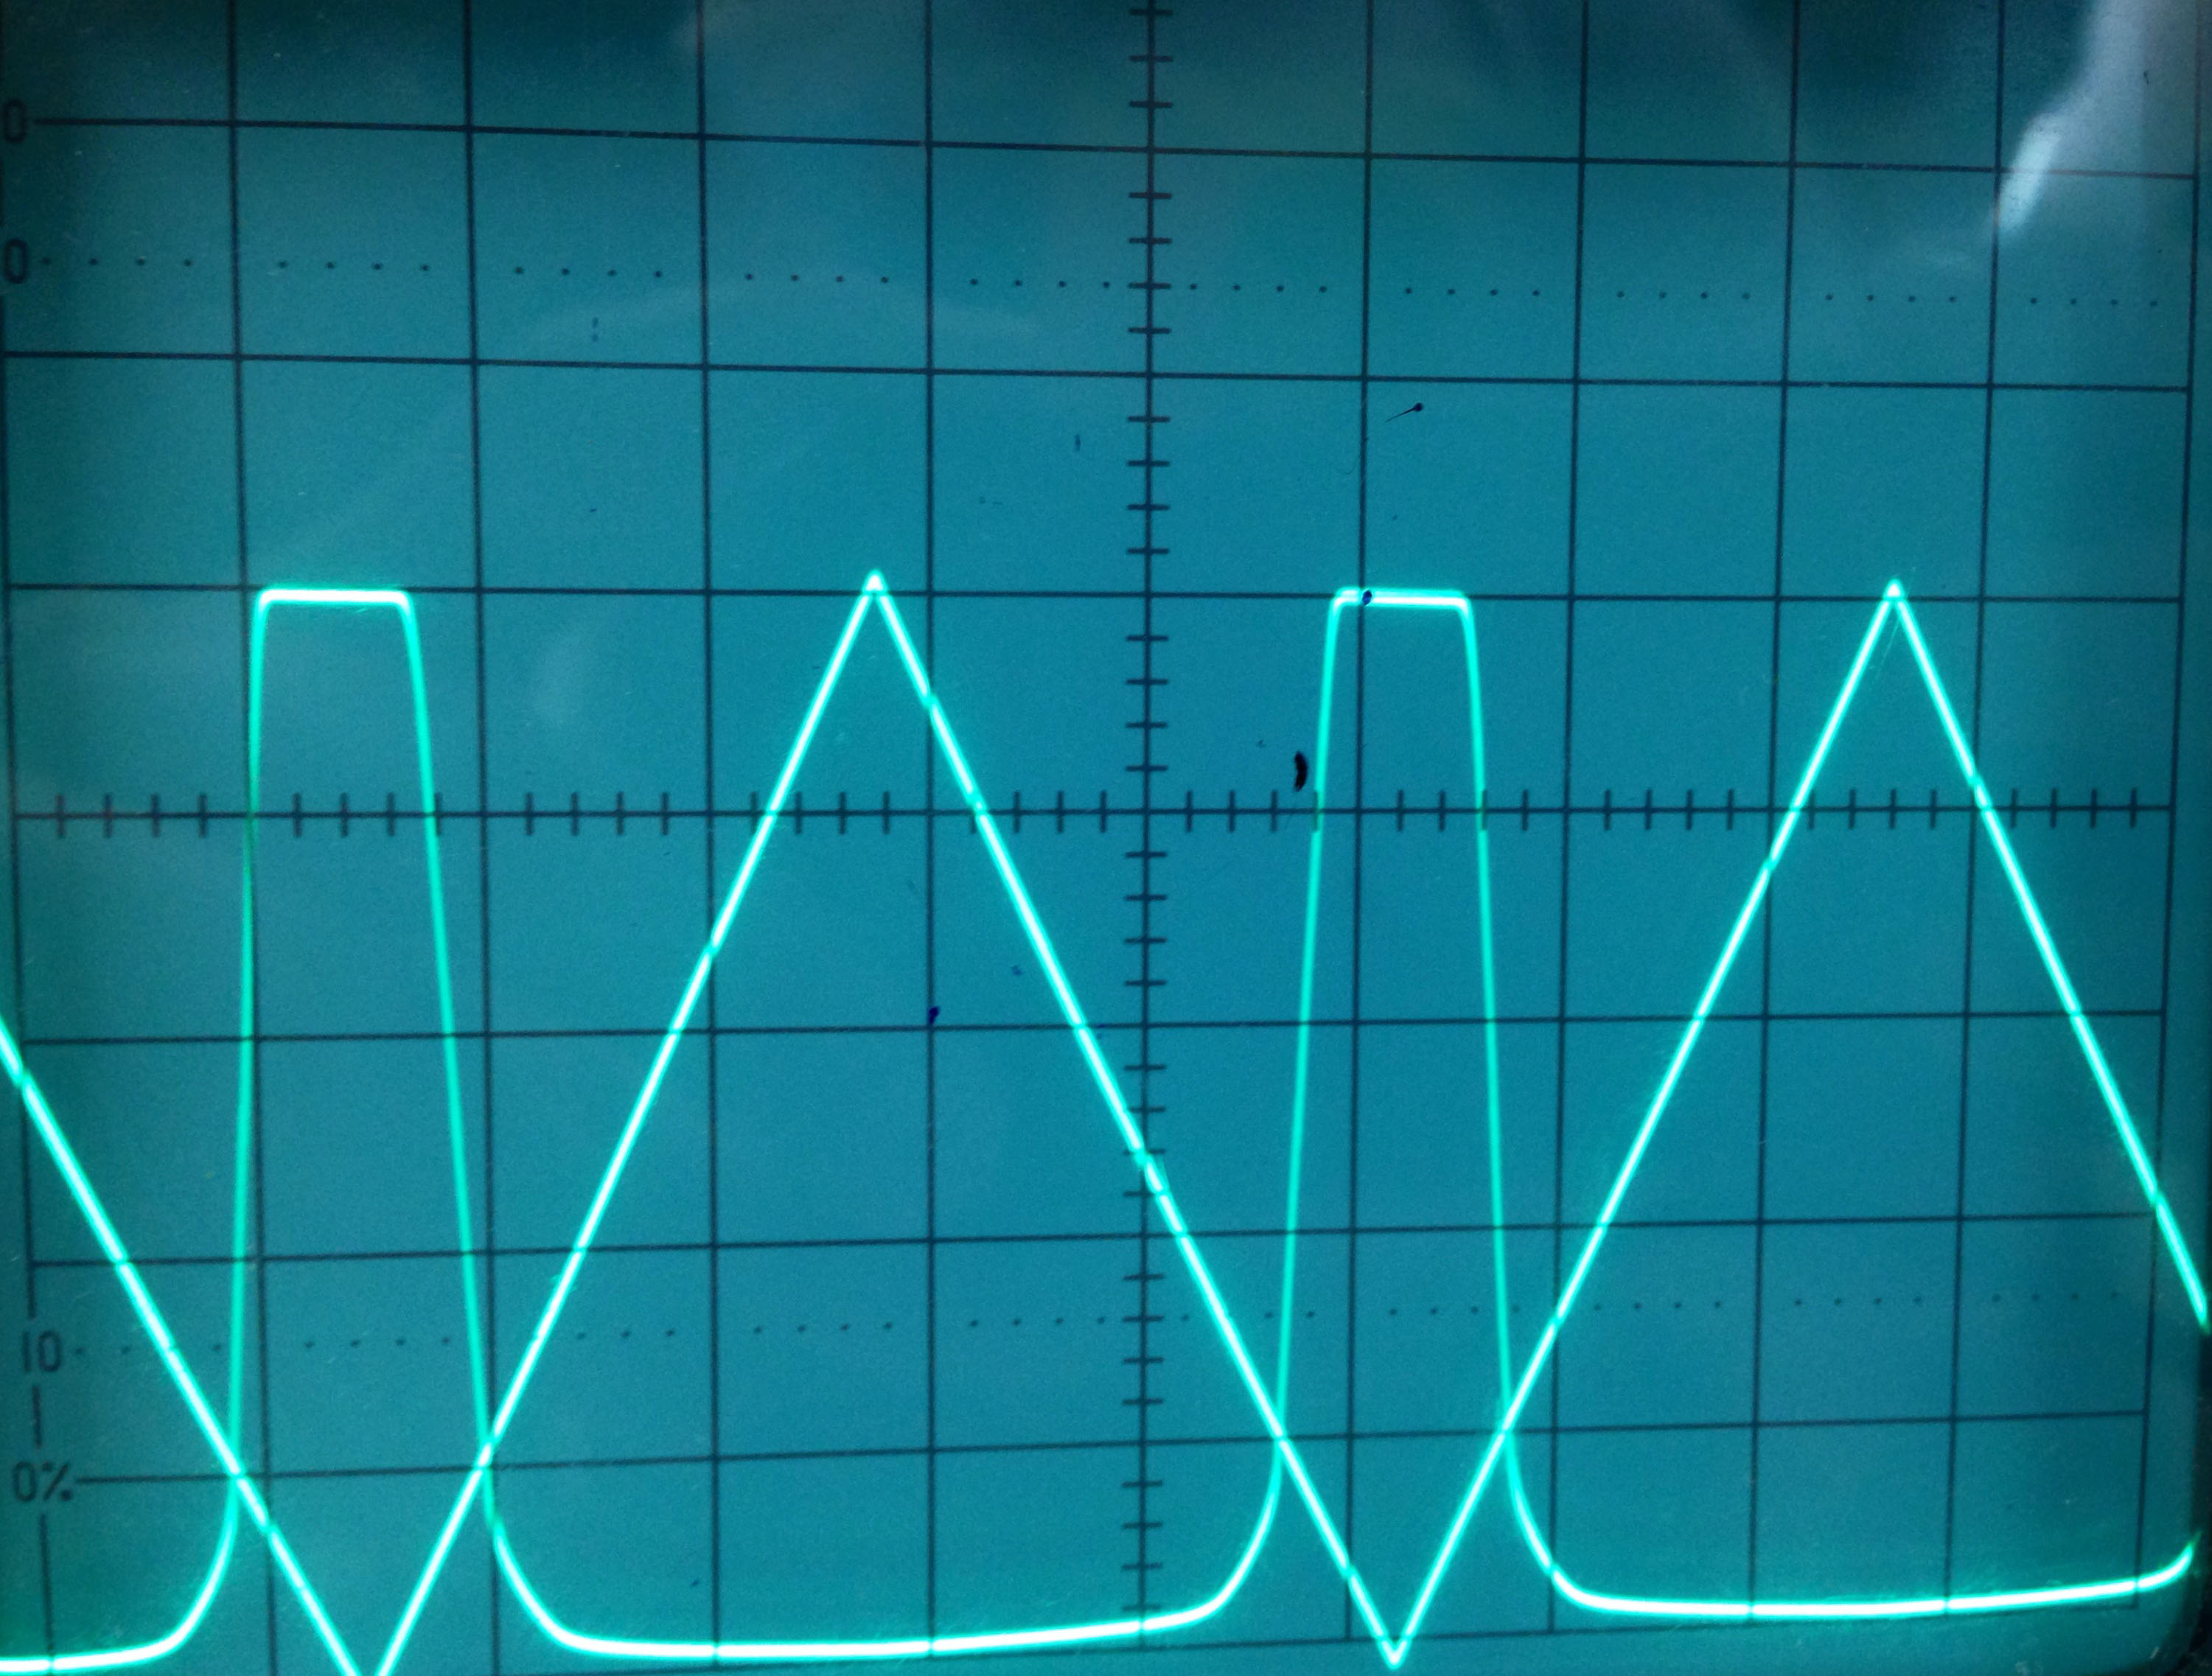
\includegraphics[width=0.8\textwidth]{./Imagens/BJT.jpg}}}
  \caption{\\Função lógica \\implementada pelo BJT. \\Vertical: 1V/div (ambos); \\Horizontal: 0,2ms/div (Time A)}\label{bjt}
\endminipage\hfill
\minipage{0.5\textwidth}
  \centerline{\fbox{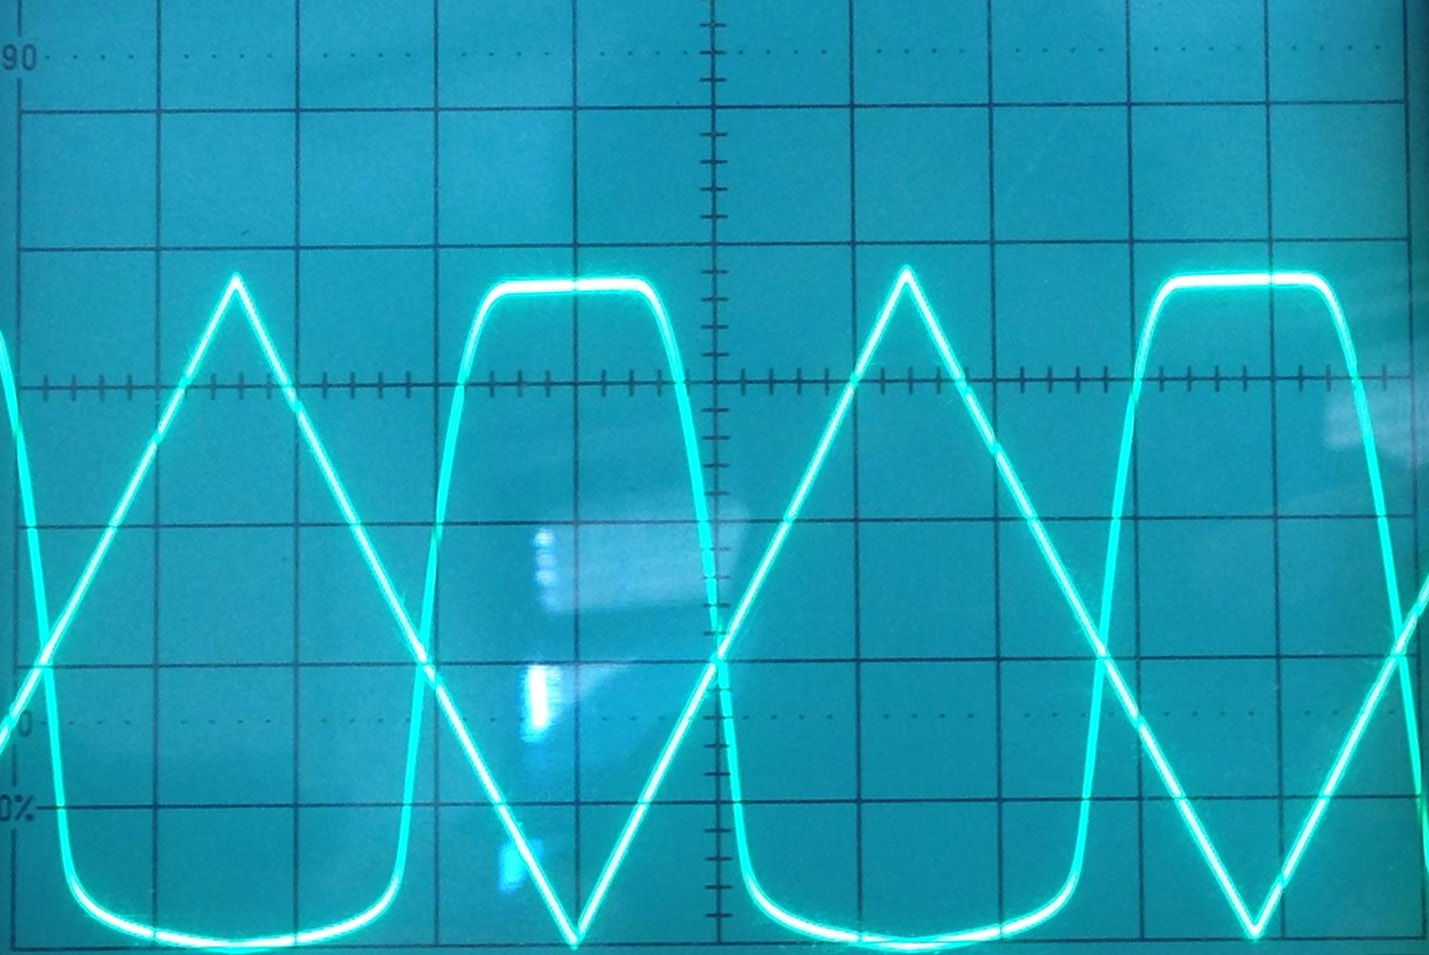
\includegraphics[width=0.8\textwidth]{Imagens/NMOS.jpg}}}
  \caption{\\Função lógica \\implementada pelo NMOS. \\Vertical: 1V/div (ambos); \\Horizontal: 0,2ms/div (Time A)}\label{fig:nmos}
\endminipage\hfill
\end{figure}

\newpage
Para o PMOS quando $V_{in}$ é 0 lógico (0V), $V_{OUT}$ é igual a $V_{DD}$.

\begin{figure}[h]
  \centerline{\fbox{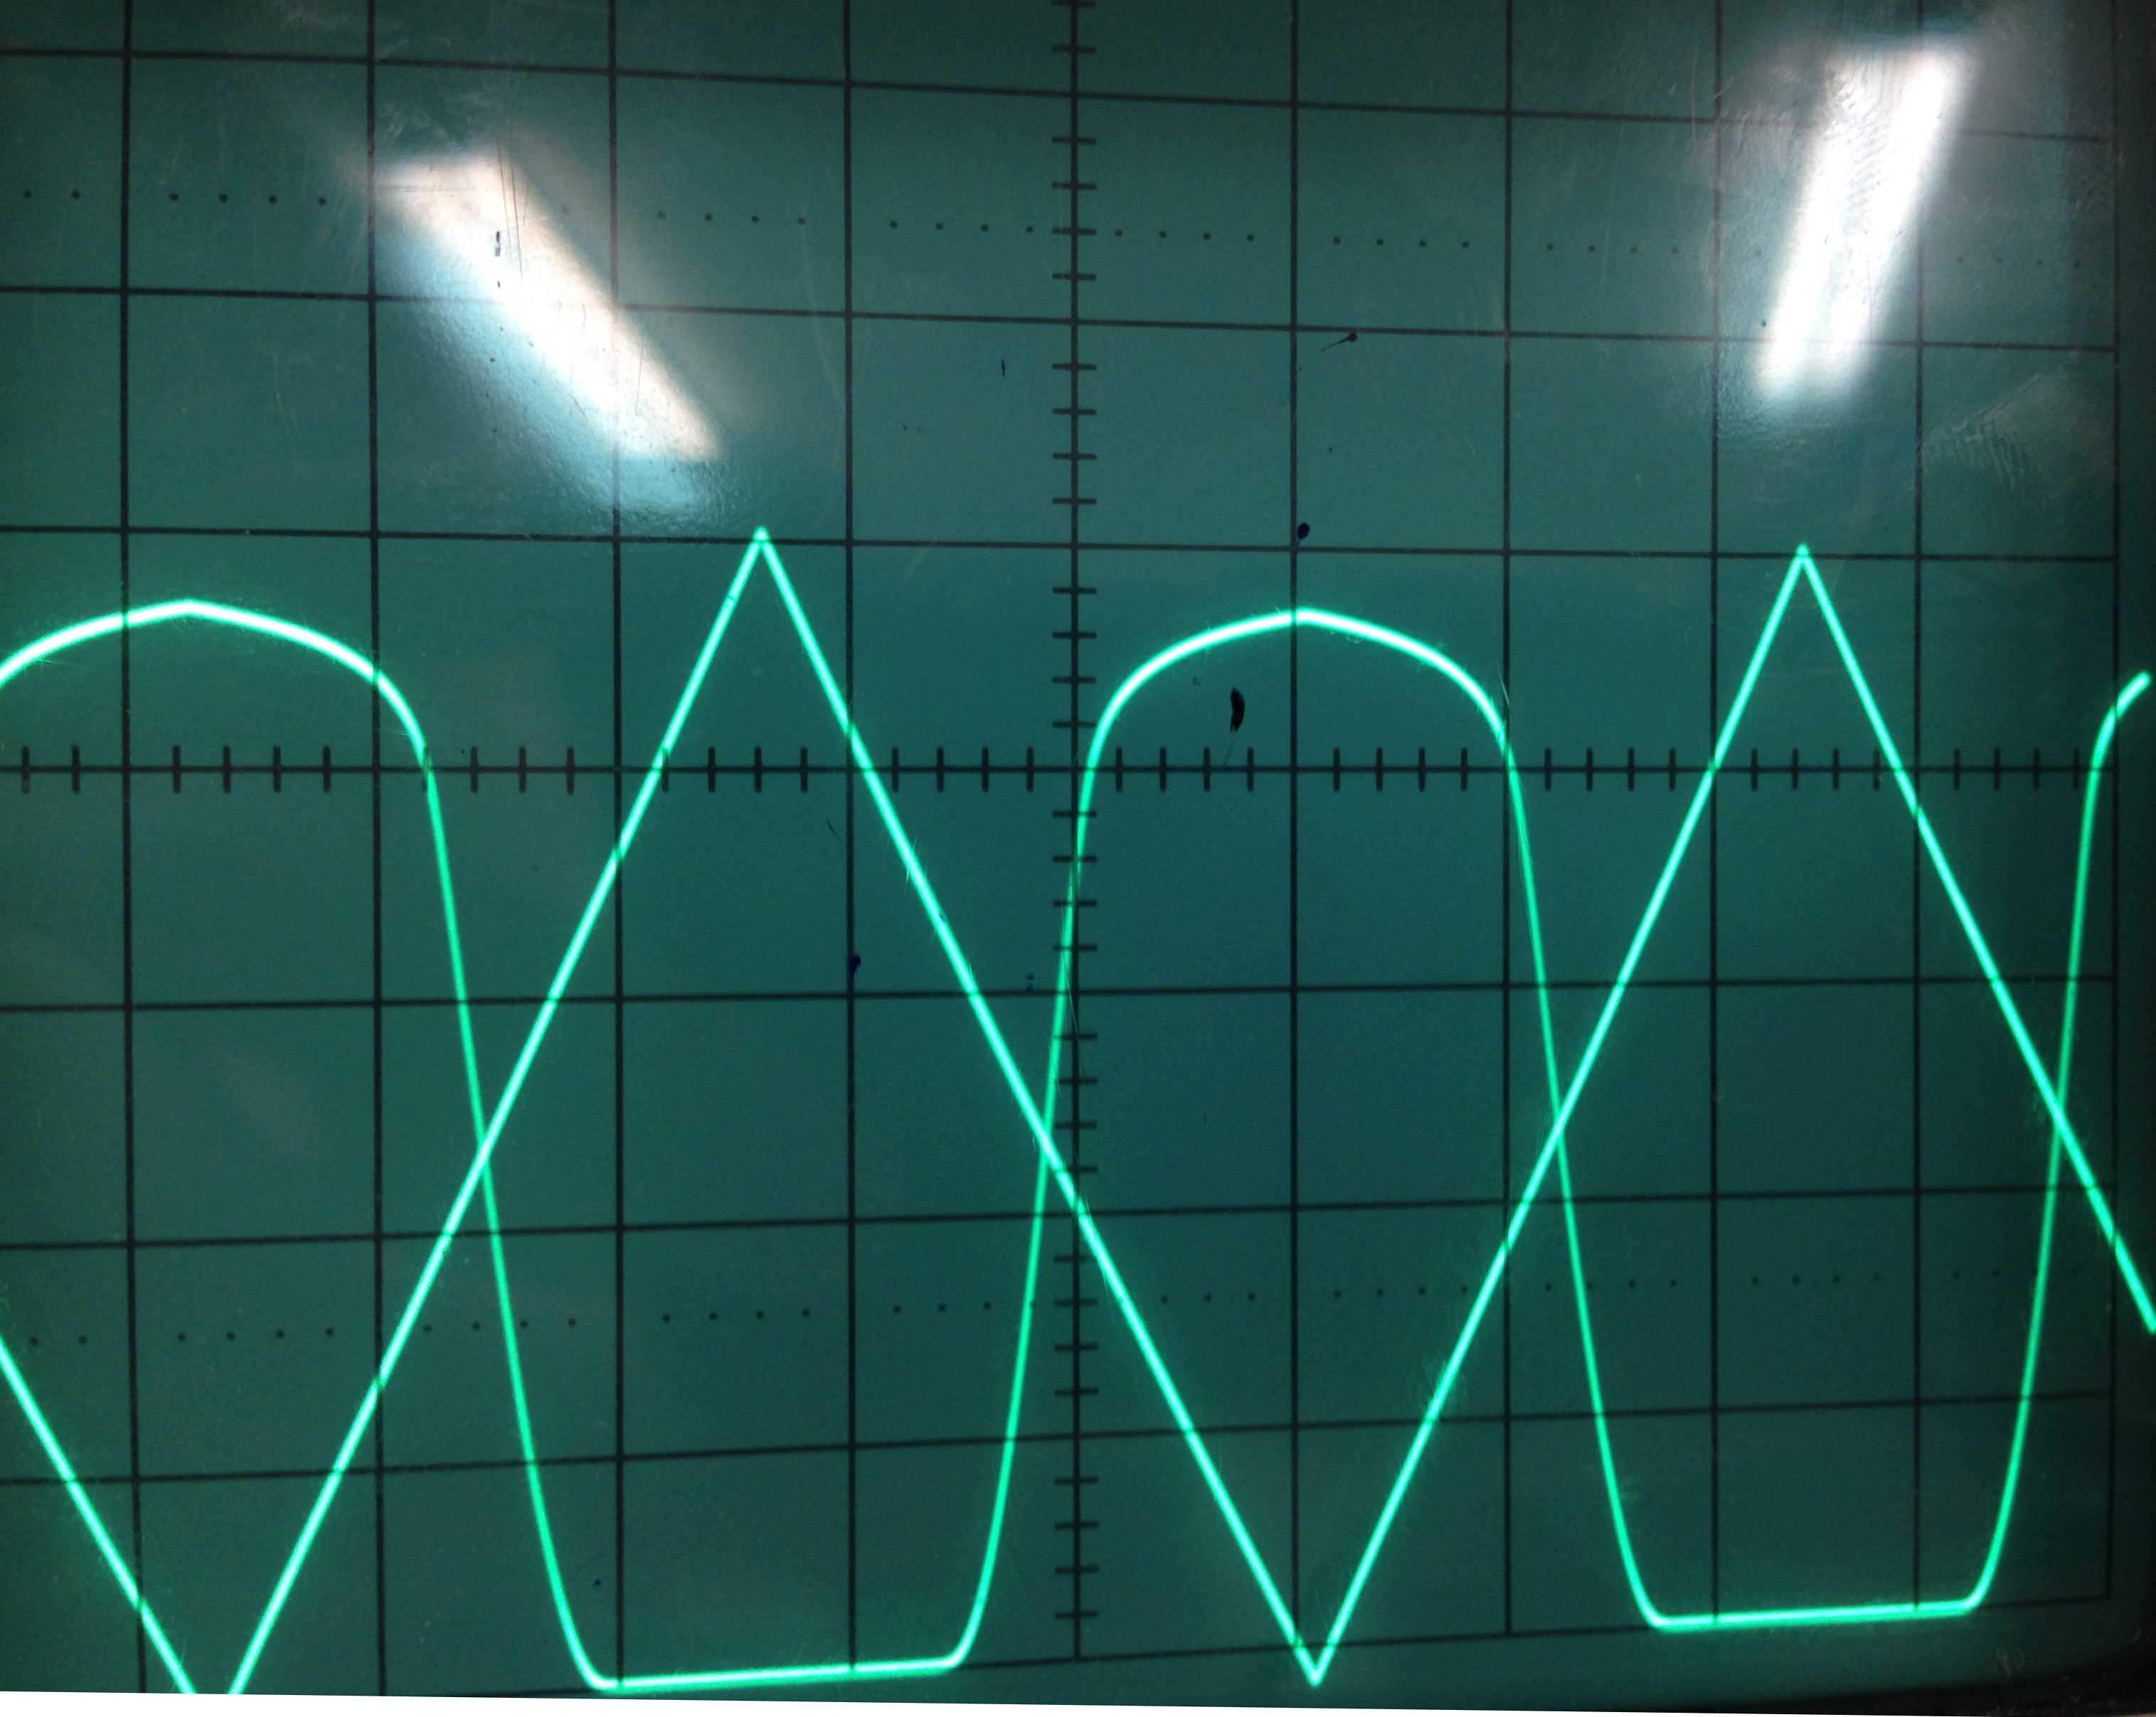
\includegraphics[width=0.5\textwidth]{./Imagens/pmos_grafico.jpg}}}
  \caption{Função lógica implementada pelo PMOS. \\Vertical: 1V/div (ambos); Horizontal: 0,1ms/div (Time A)}\label{cmos}
\end{figure}

No CMOS se o $V_{in}$ for igual a 0 lógico (0V), em $M_1$ deixa fluir corrente passando $V_{DD}$ e $M_2$ fica em corte, ficando portanto $V_{OUT}$ = $V_{DD}$.

\begin{figure}[h]
  \centerline{\fbox{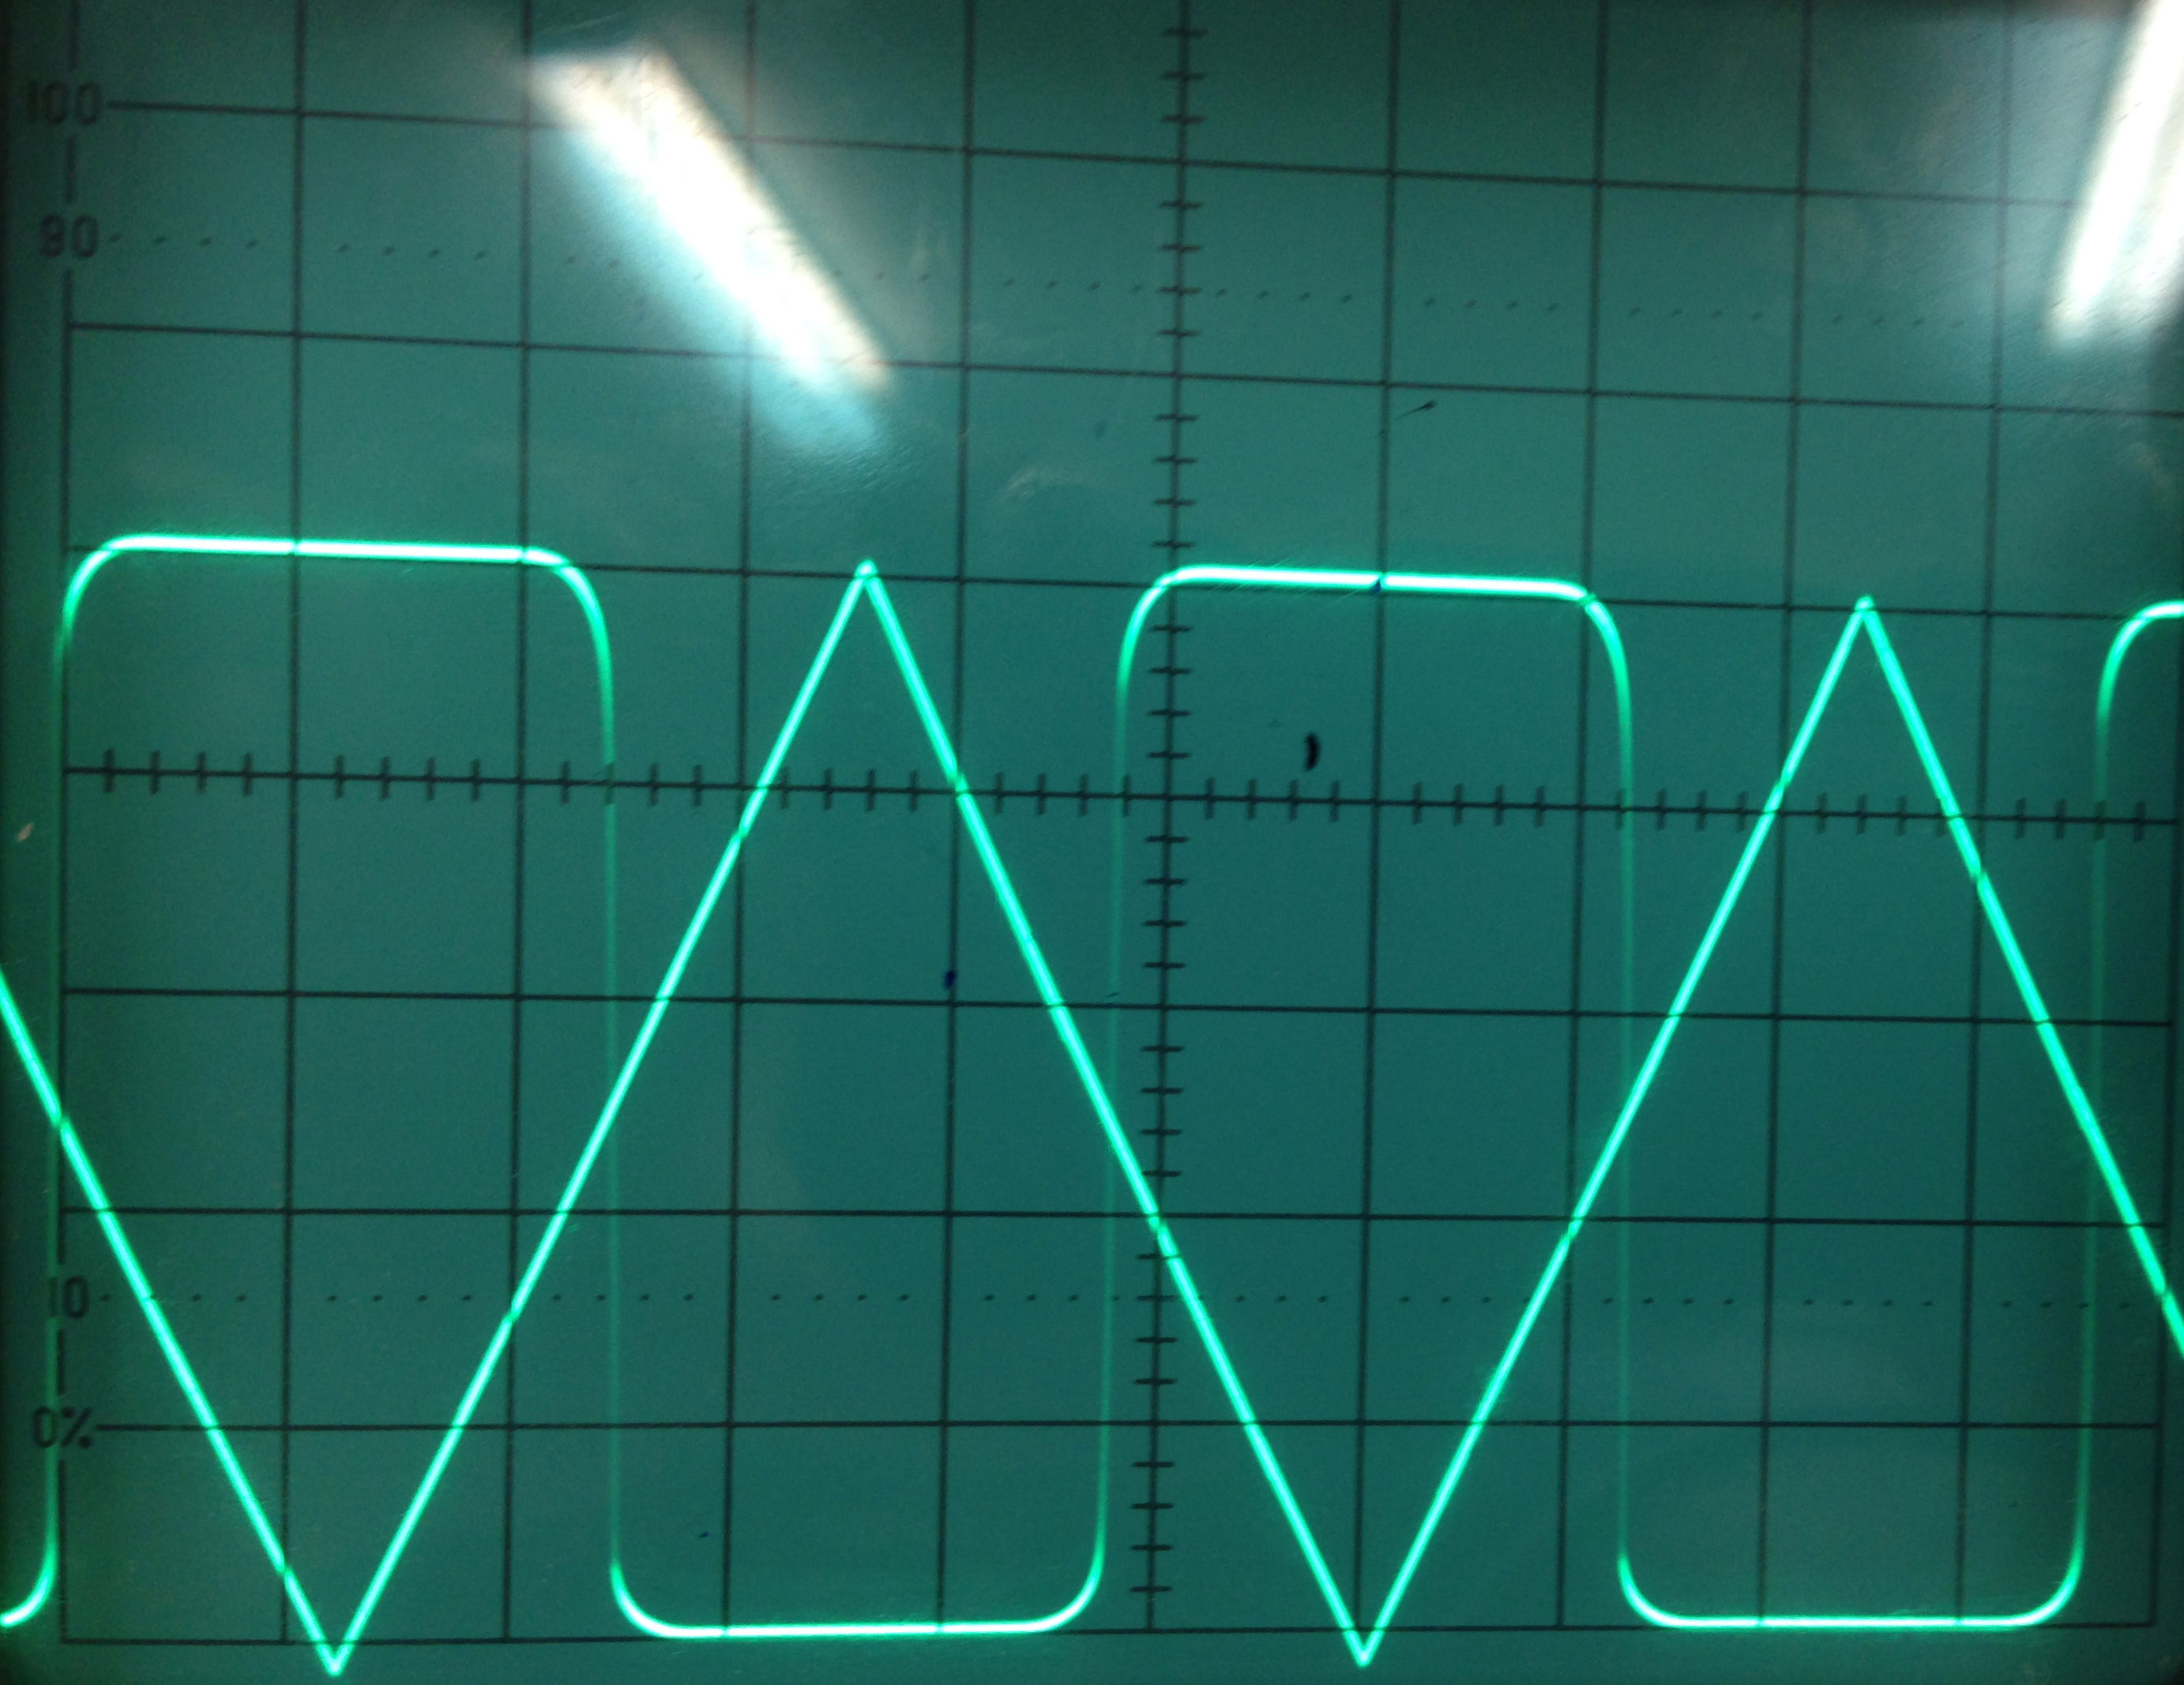
\includegraphics[width=0.5\textwidth]{./Imagens/cmos_grafico.jpg}}}
  \caption{\\Função lógica implementada pelo CMOS. \\Vertical: 1V/div (ambos); Horizontal: 0,1ms/div (Time A)}\label{cmos}
\end{figure}

\newpage
\subsection{Voltage Transfer Characteristic (VTC) de cada um dos circuitos}
\begin{figure}[!htb]
\minipage{0.5\textwidth}
  \centerline{\fbox{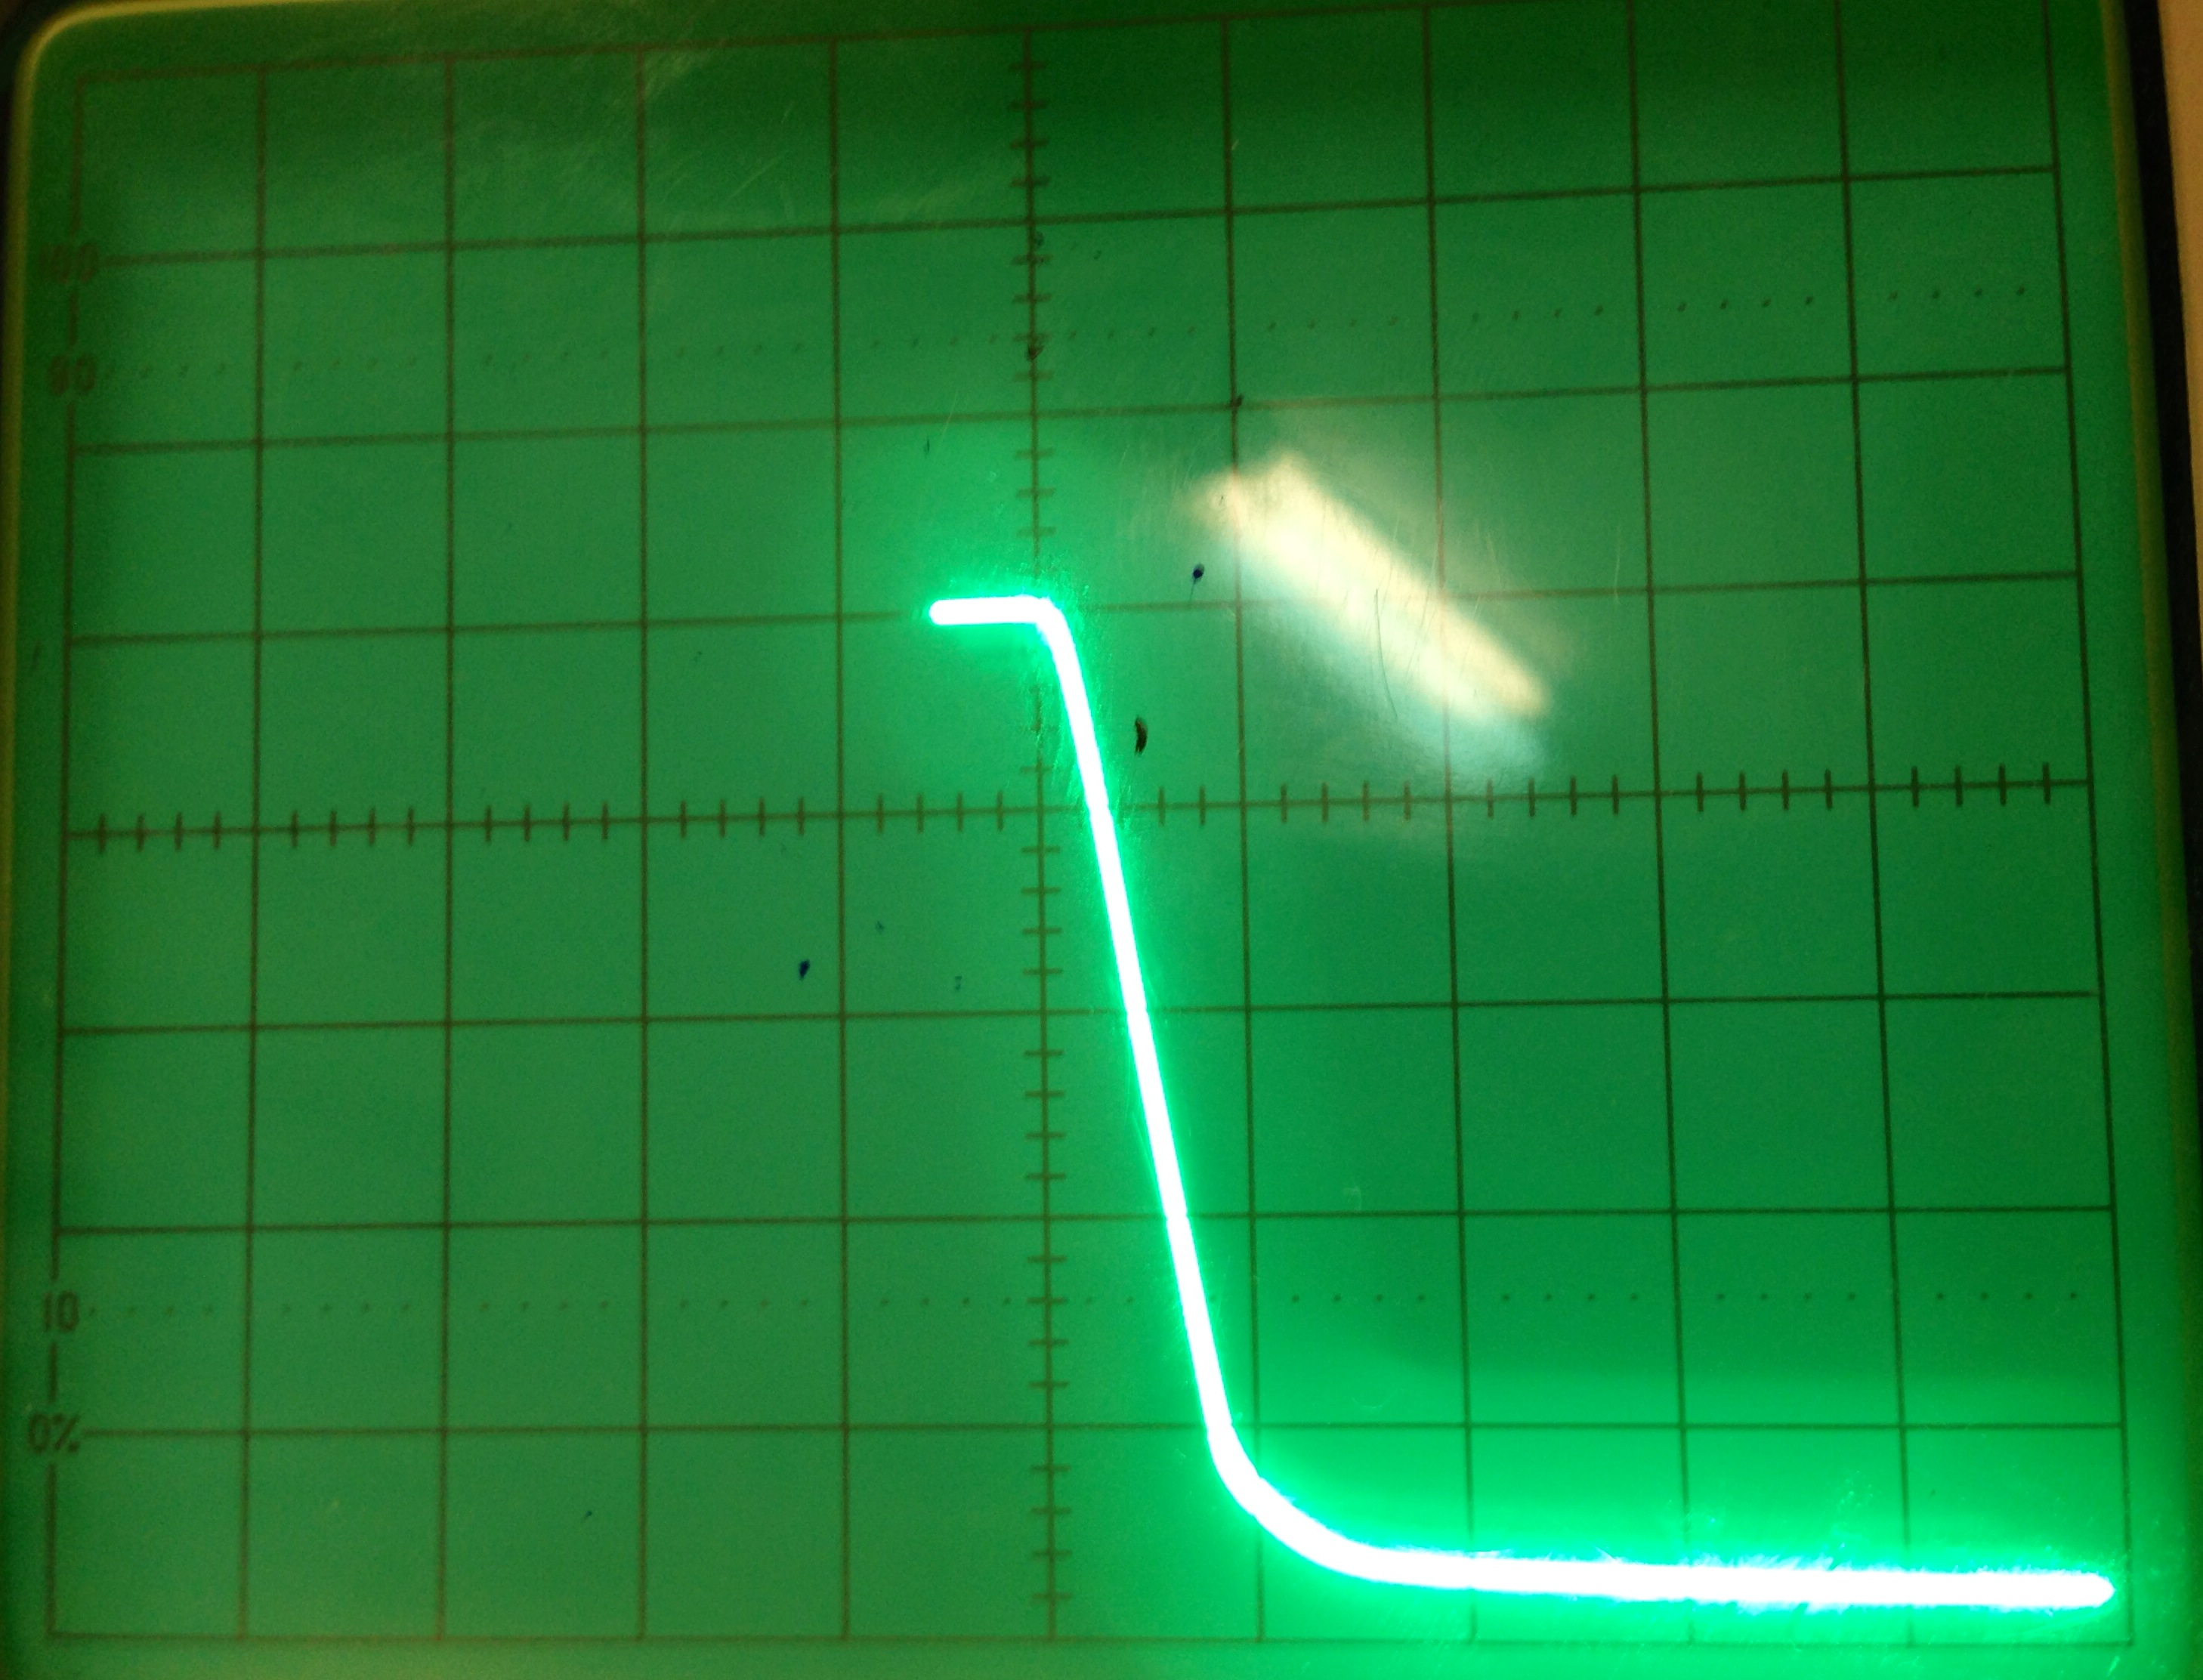
\includegraphics[width=0.8\textwidth]{./Imagens/bjt_vtc.jpg}}}
  \caption{\\VTC BJT \\Vertical: 1V/div (ambos); \\Horizontal: 0,2ms/div (Time A)}\label{bjt}
\endminipage\hfill
\minipage{0.5\textwidth}
  \centerline{\fbox{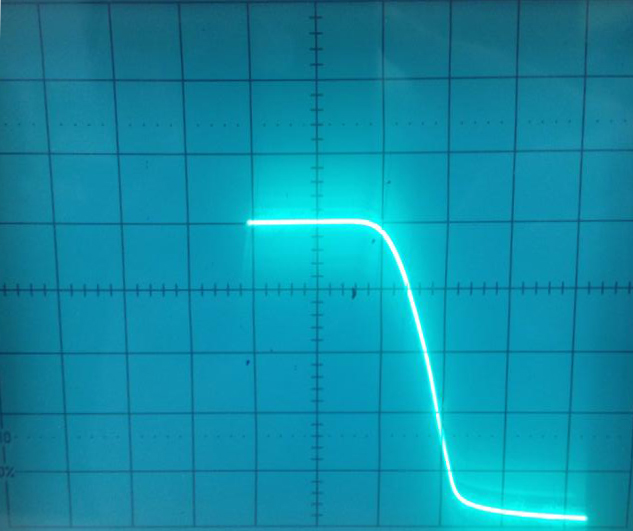
\includegraphics[width=0.8\textwidth]{Imagens/nmos_vtc.jpg}}}
  \caption{\\VTC NMOS \\Vertical: 1V/div ; \\Horizontal: 1V/div }\label{fig:nmos}
\endminipage\hfill
\end{figure}

\begin{figure}[!htb]
\minipage{0.5\textwidth}
  \centerline{\fbox{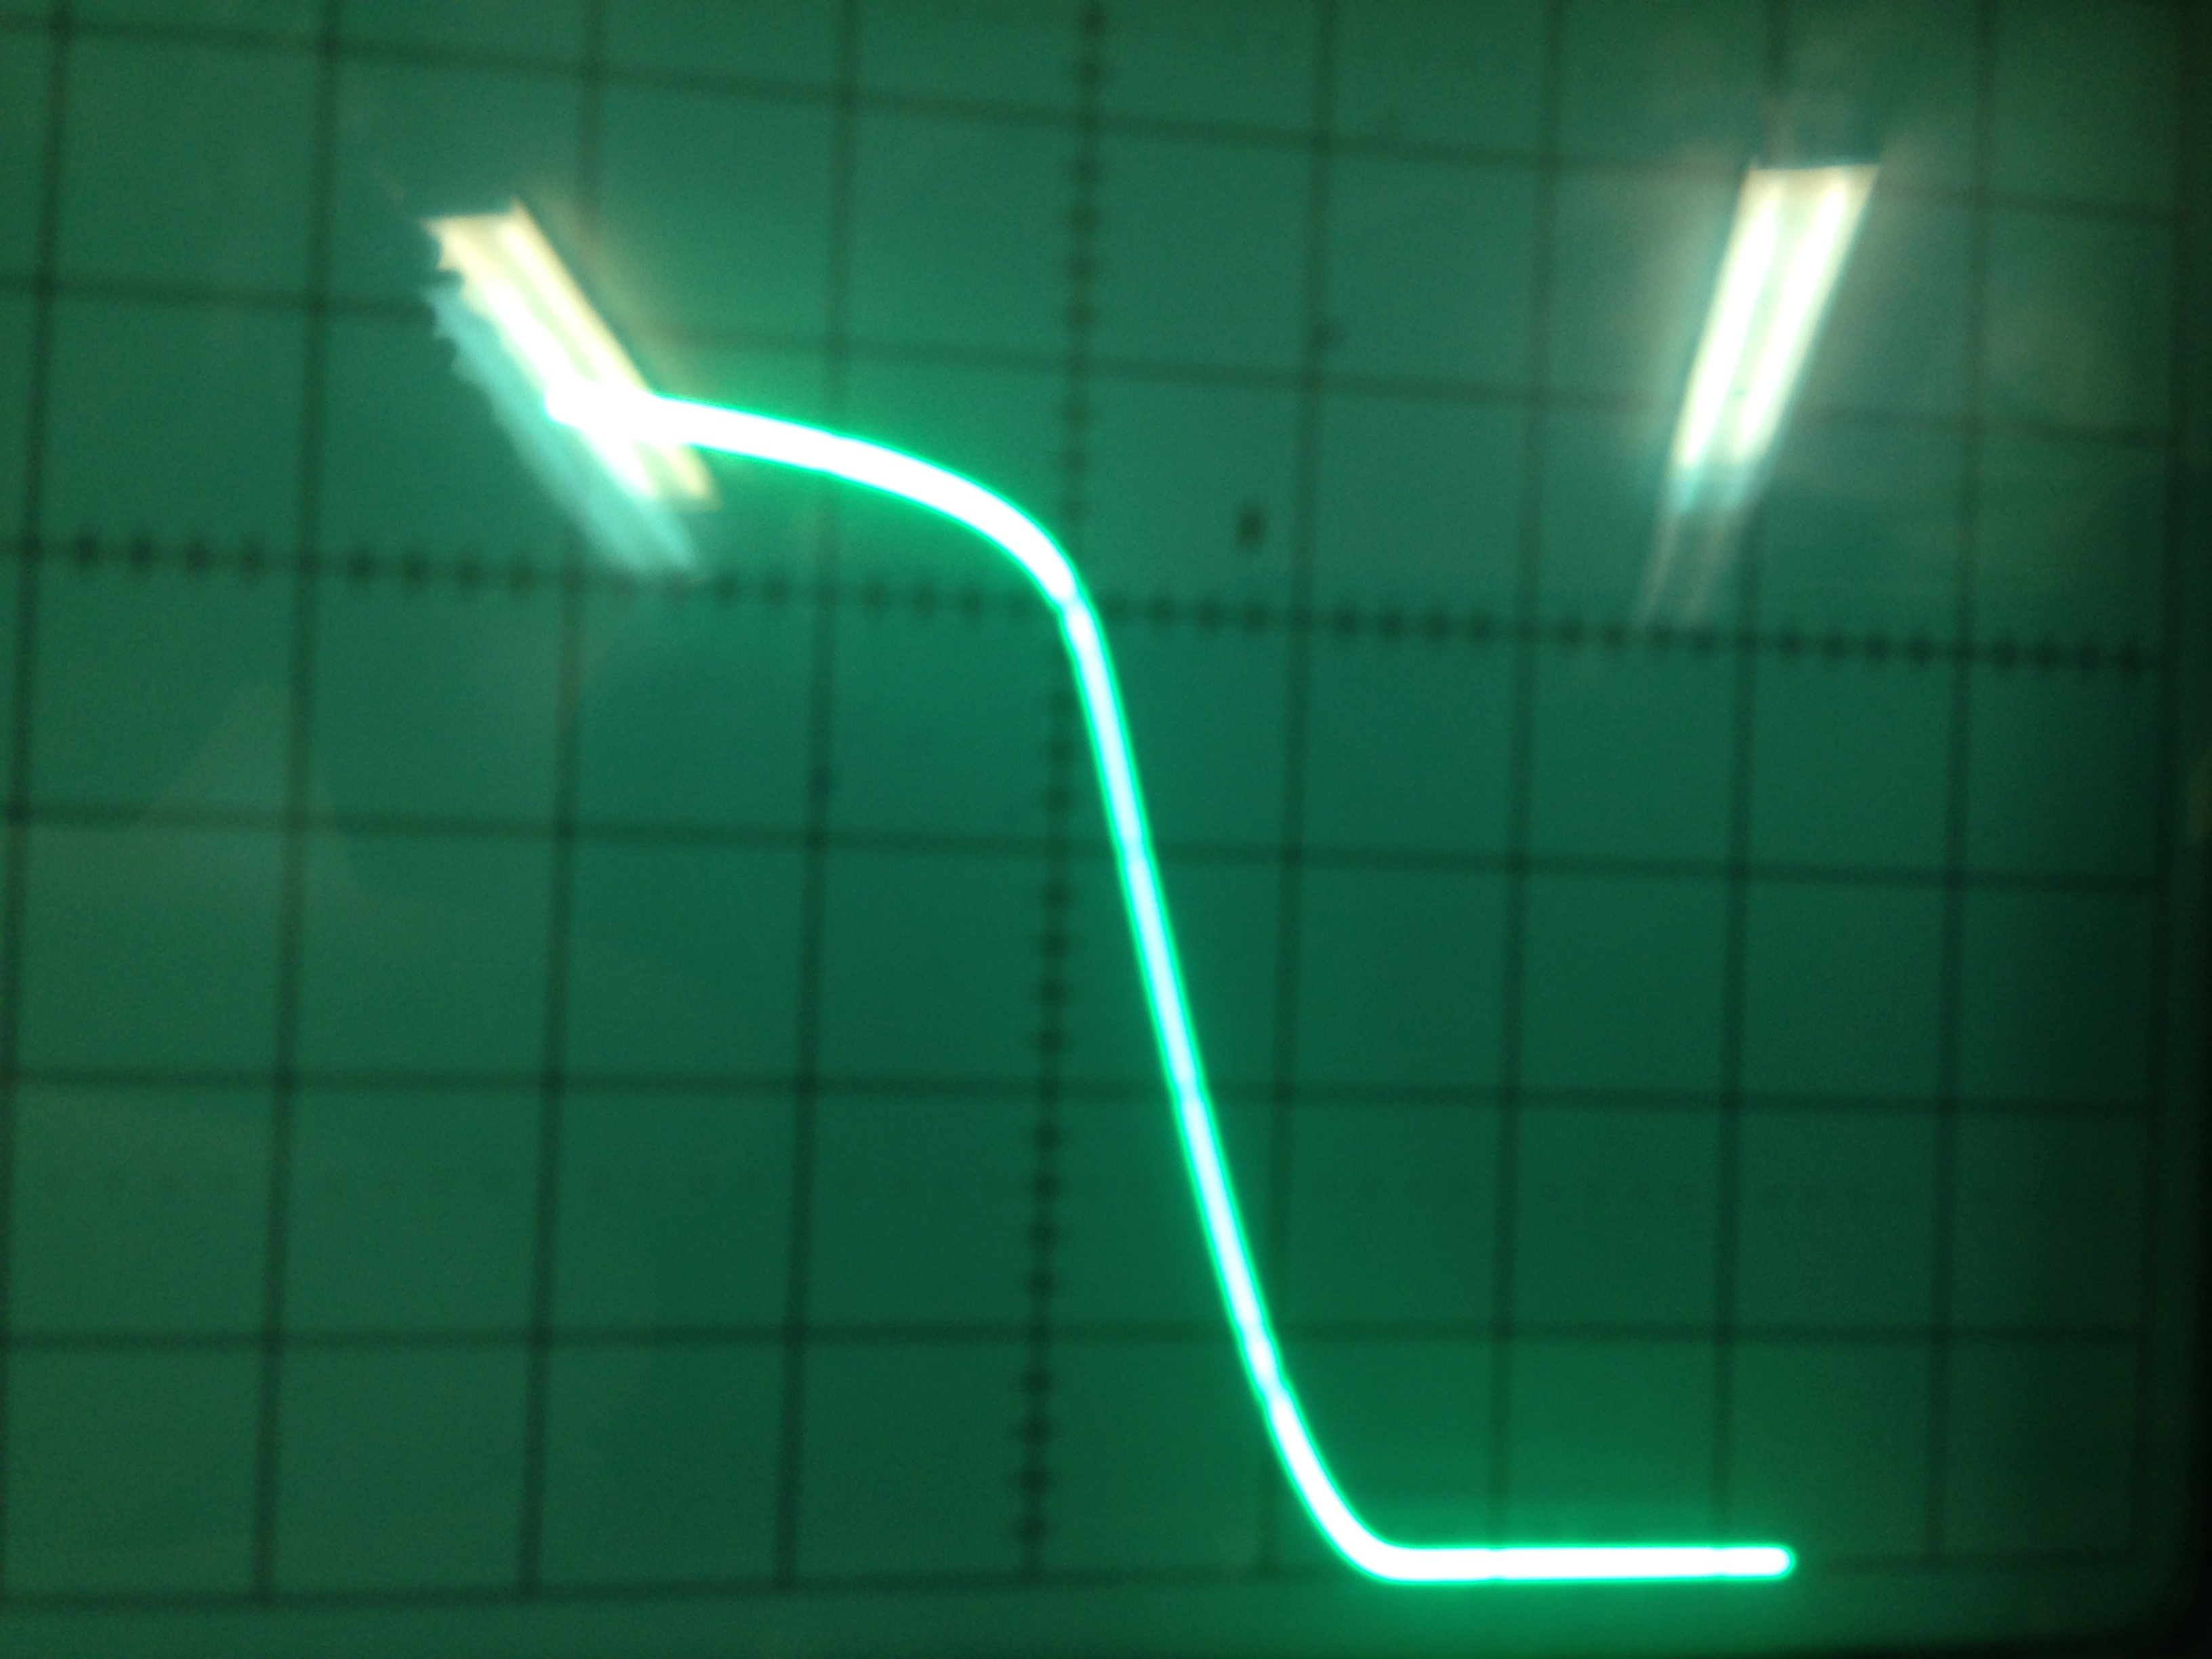
\includegraphics[width=0.8\textwidth]{Imagens/pmos_vtc.jpg}}}
  \caption{\\VTC PMOS \\Vertical: 1V/div ($V_{out}$); \\Horizontal: 1V/div ($V_{in}$)}
\endminipage\hfill
\minipage{0.5\textwidth}
  \centerline{\fbox{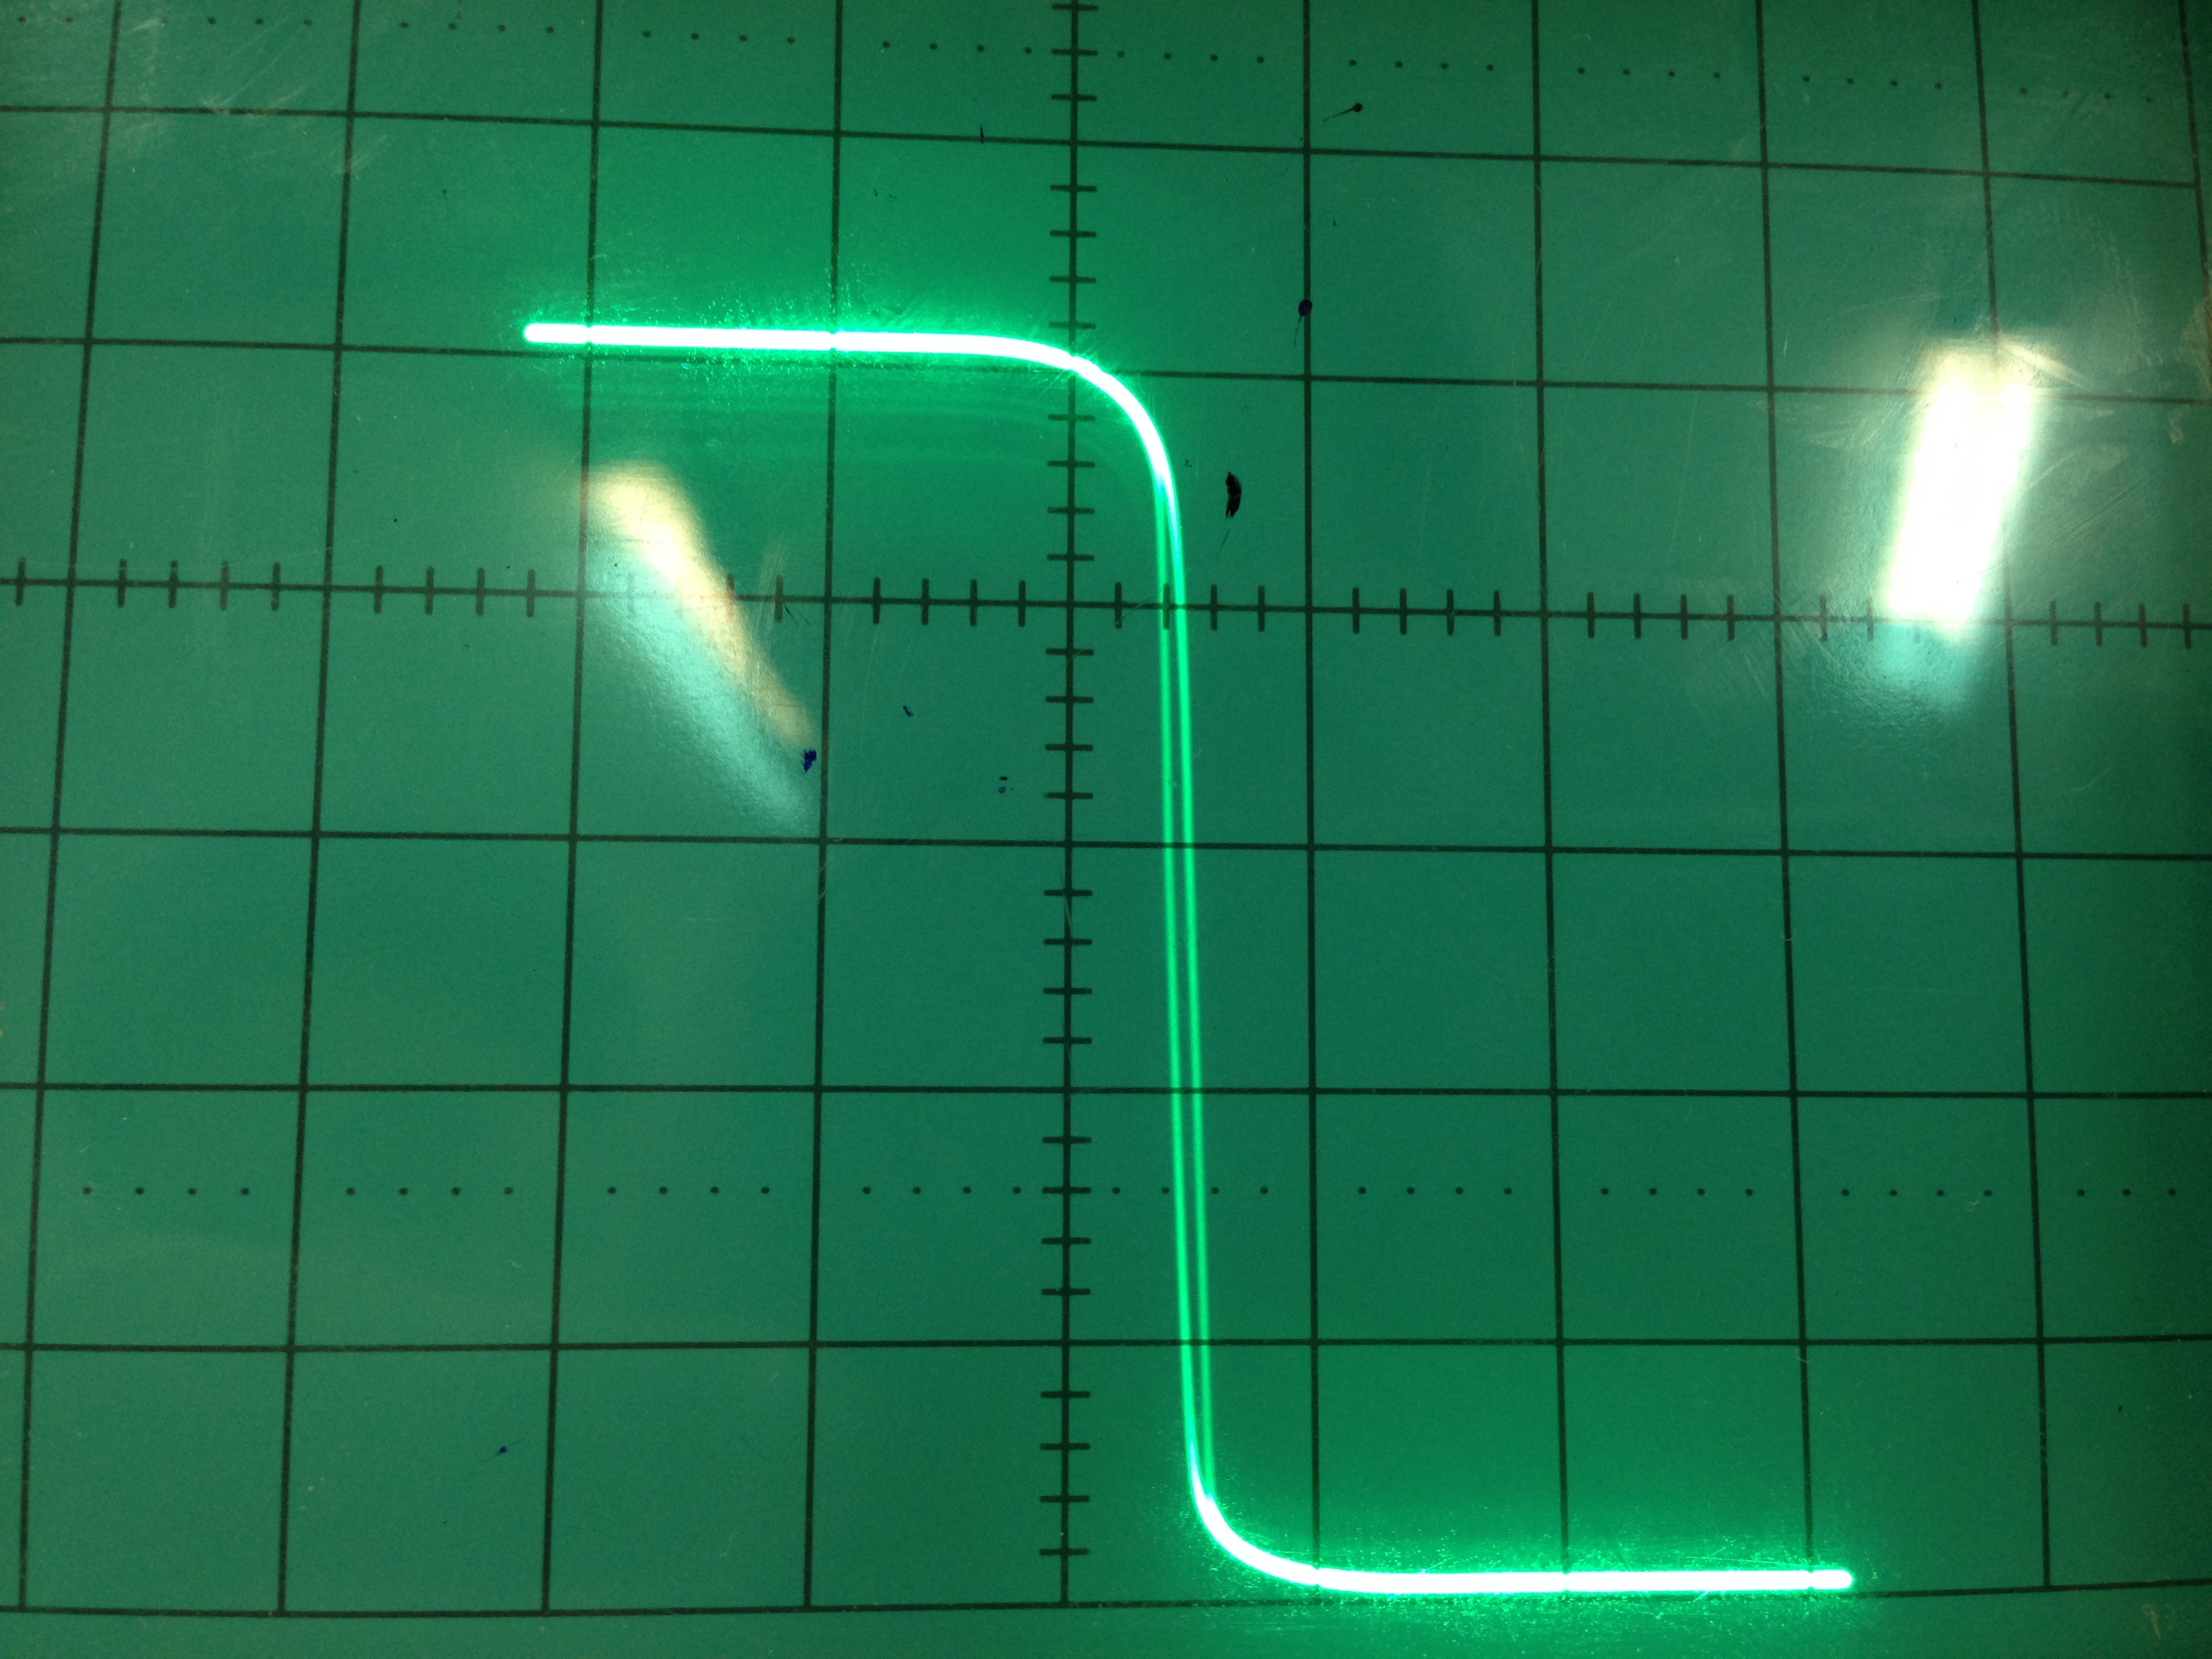
\includegraphics[width=0.8\textwidth]{Imagens/cmos_vtc.jpg}}}
  \caption{\\VTC CMOS \\Vertical: 1V/div ($V_{out}$); \\Horizontal: 1V/div ($V_{in}$)}
\endminipage\hfill
\end{figure}

\newpage
\subsection{Comparação dos VTC das quatro portas}
Através das imagens acima, observa-se que a porta CMOS é a mais ideal na mudança do nível lógico. Ao contrário das outras portas, em que temos durante algum tempo zona de saturação na mudança de nível, no CMOS, esta alteração é repentina, daí ser a porta mais ideal. Esta situação é explicada pelo facto de que o CMOS é construído com base nas portas NMOS e PMOS, ou seja, quando um está a conduzir, o outro está em corte, sendo que apenas em  $\frac{V_{DD}}{2}$ ambas se encontram em saturação.

\subsection{Medição e comparação do tempo de subida e descida de cada gate ligando um condensador}

O tempo de subida e descida $t_{sd}$ de uma porta digital indica a rapidez com que ela responde a uma mudança nas suas entradas. O atraso associado a uma mudança H $\rightarrow$ L na saída designa-se por $t_{pHL}$ e uma mudança de L $\rightarrow$ H é $t_{pLH}$. Então o $t_{sd}$ é a media:

\centerline{$t_{sd} = \frac{t_{pHL}+t_{pLH}}{2}$}

\begin{figure}[!htb]
\minipage{0.5\textwidth}
  \centerline{\fbox{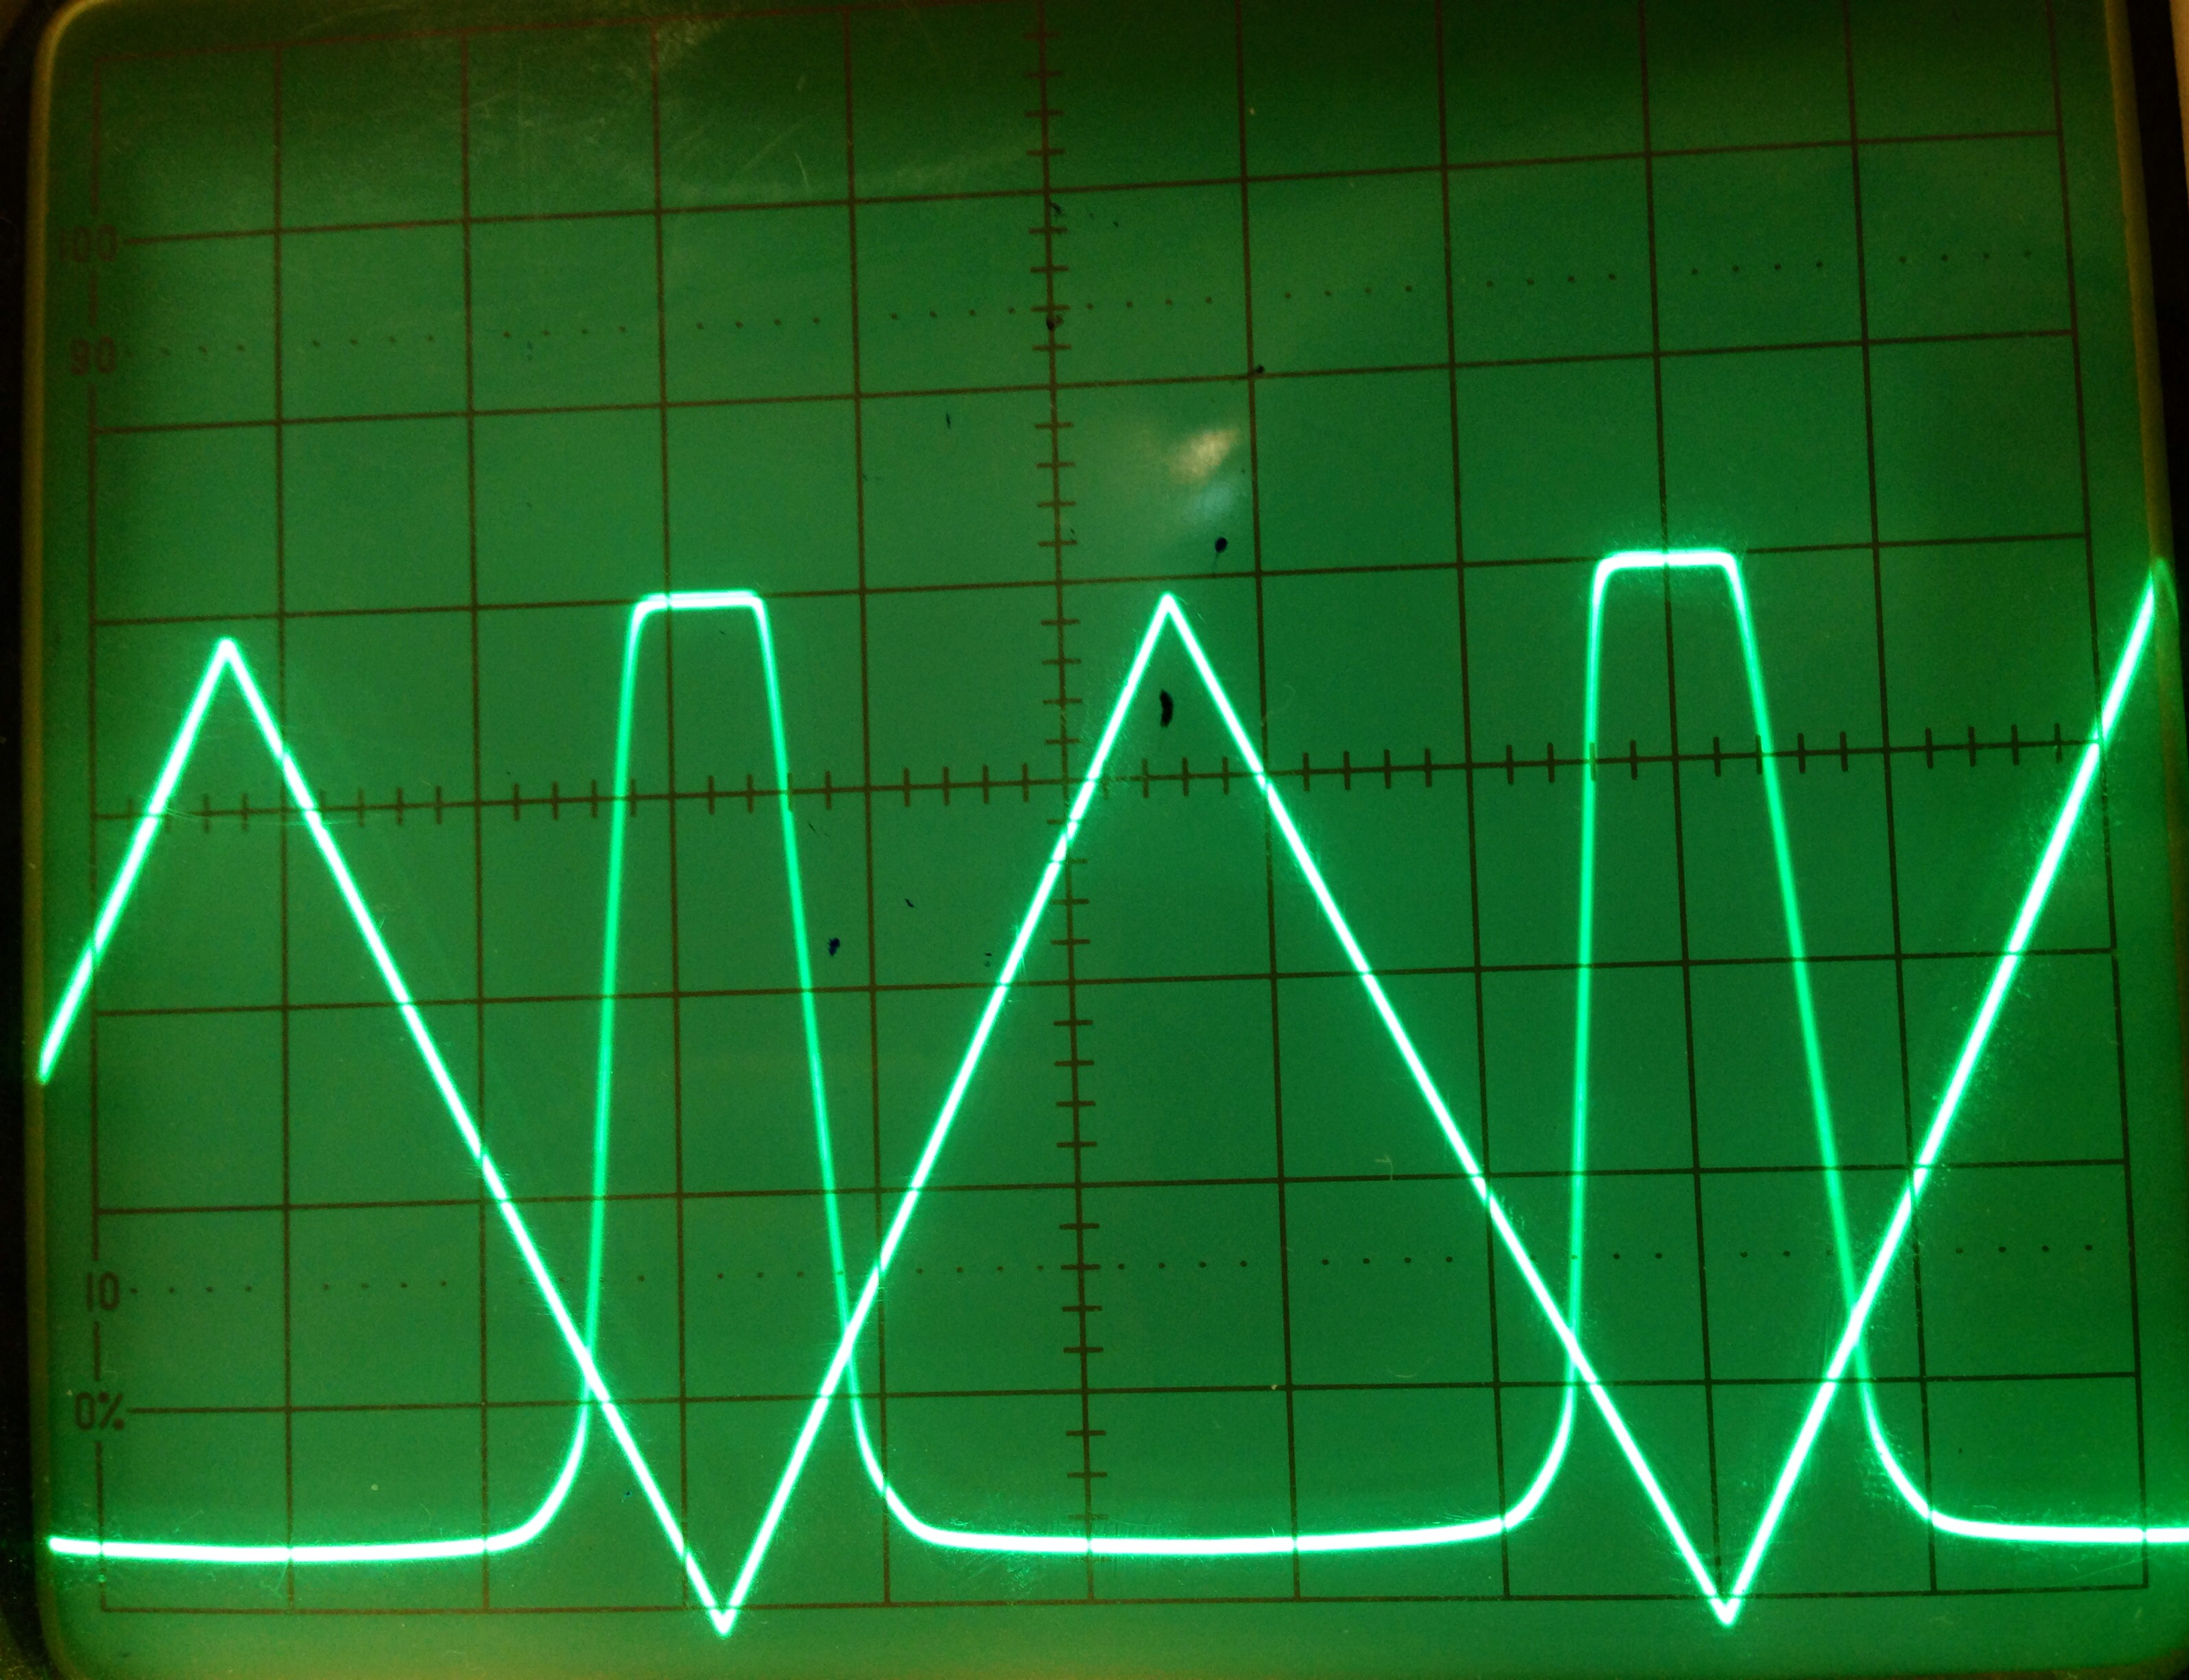
\includegraphics[width=0.8\textwidth]{./Imagens/bjt_condensador_grafico.jpg}}}
  \caption{\\Gráfico BJT com condensador\\Vertical: 1V/div (ambos); \\Horizontal: 0,2ms/div (Time A)}\label{bjt}
\endminipage\hfill
\minipage{0.5\textwidth}
  \centerline{\fbox{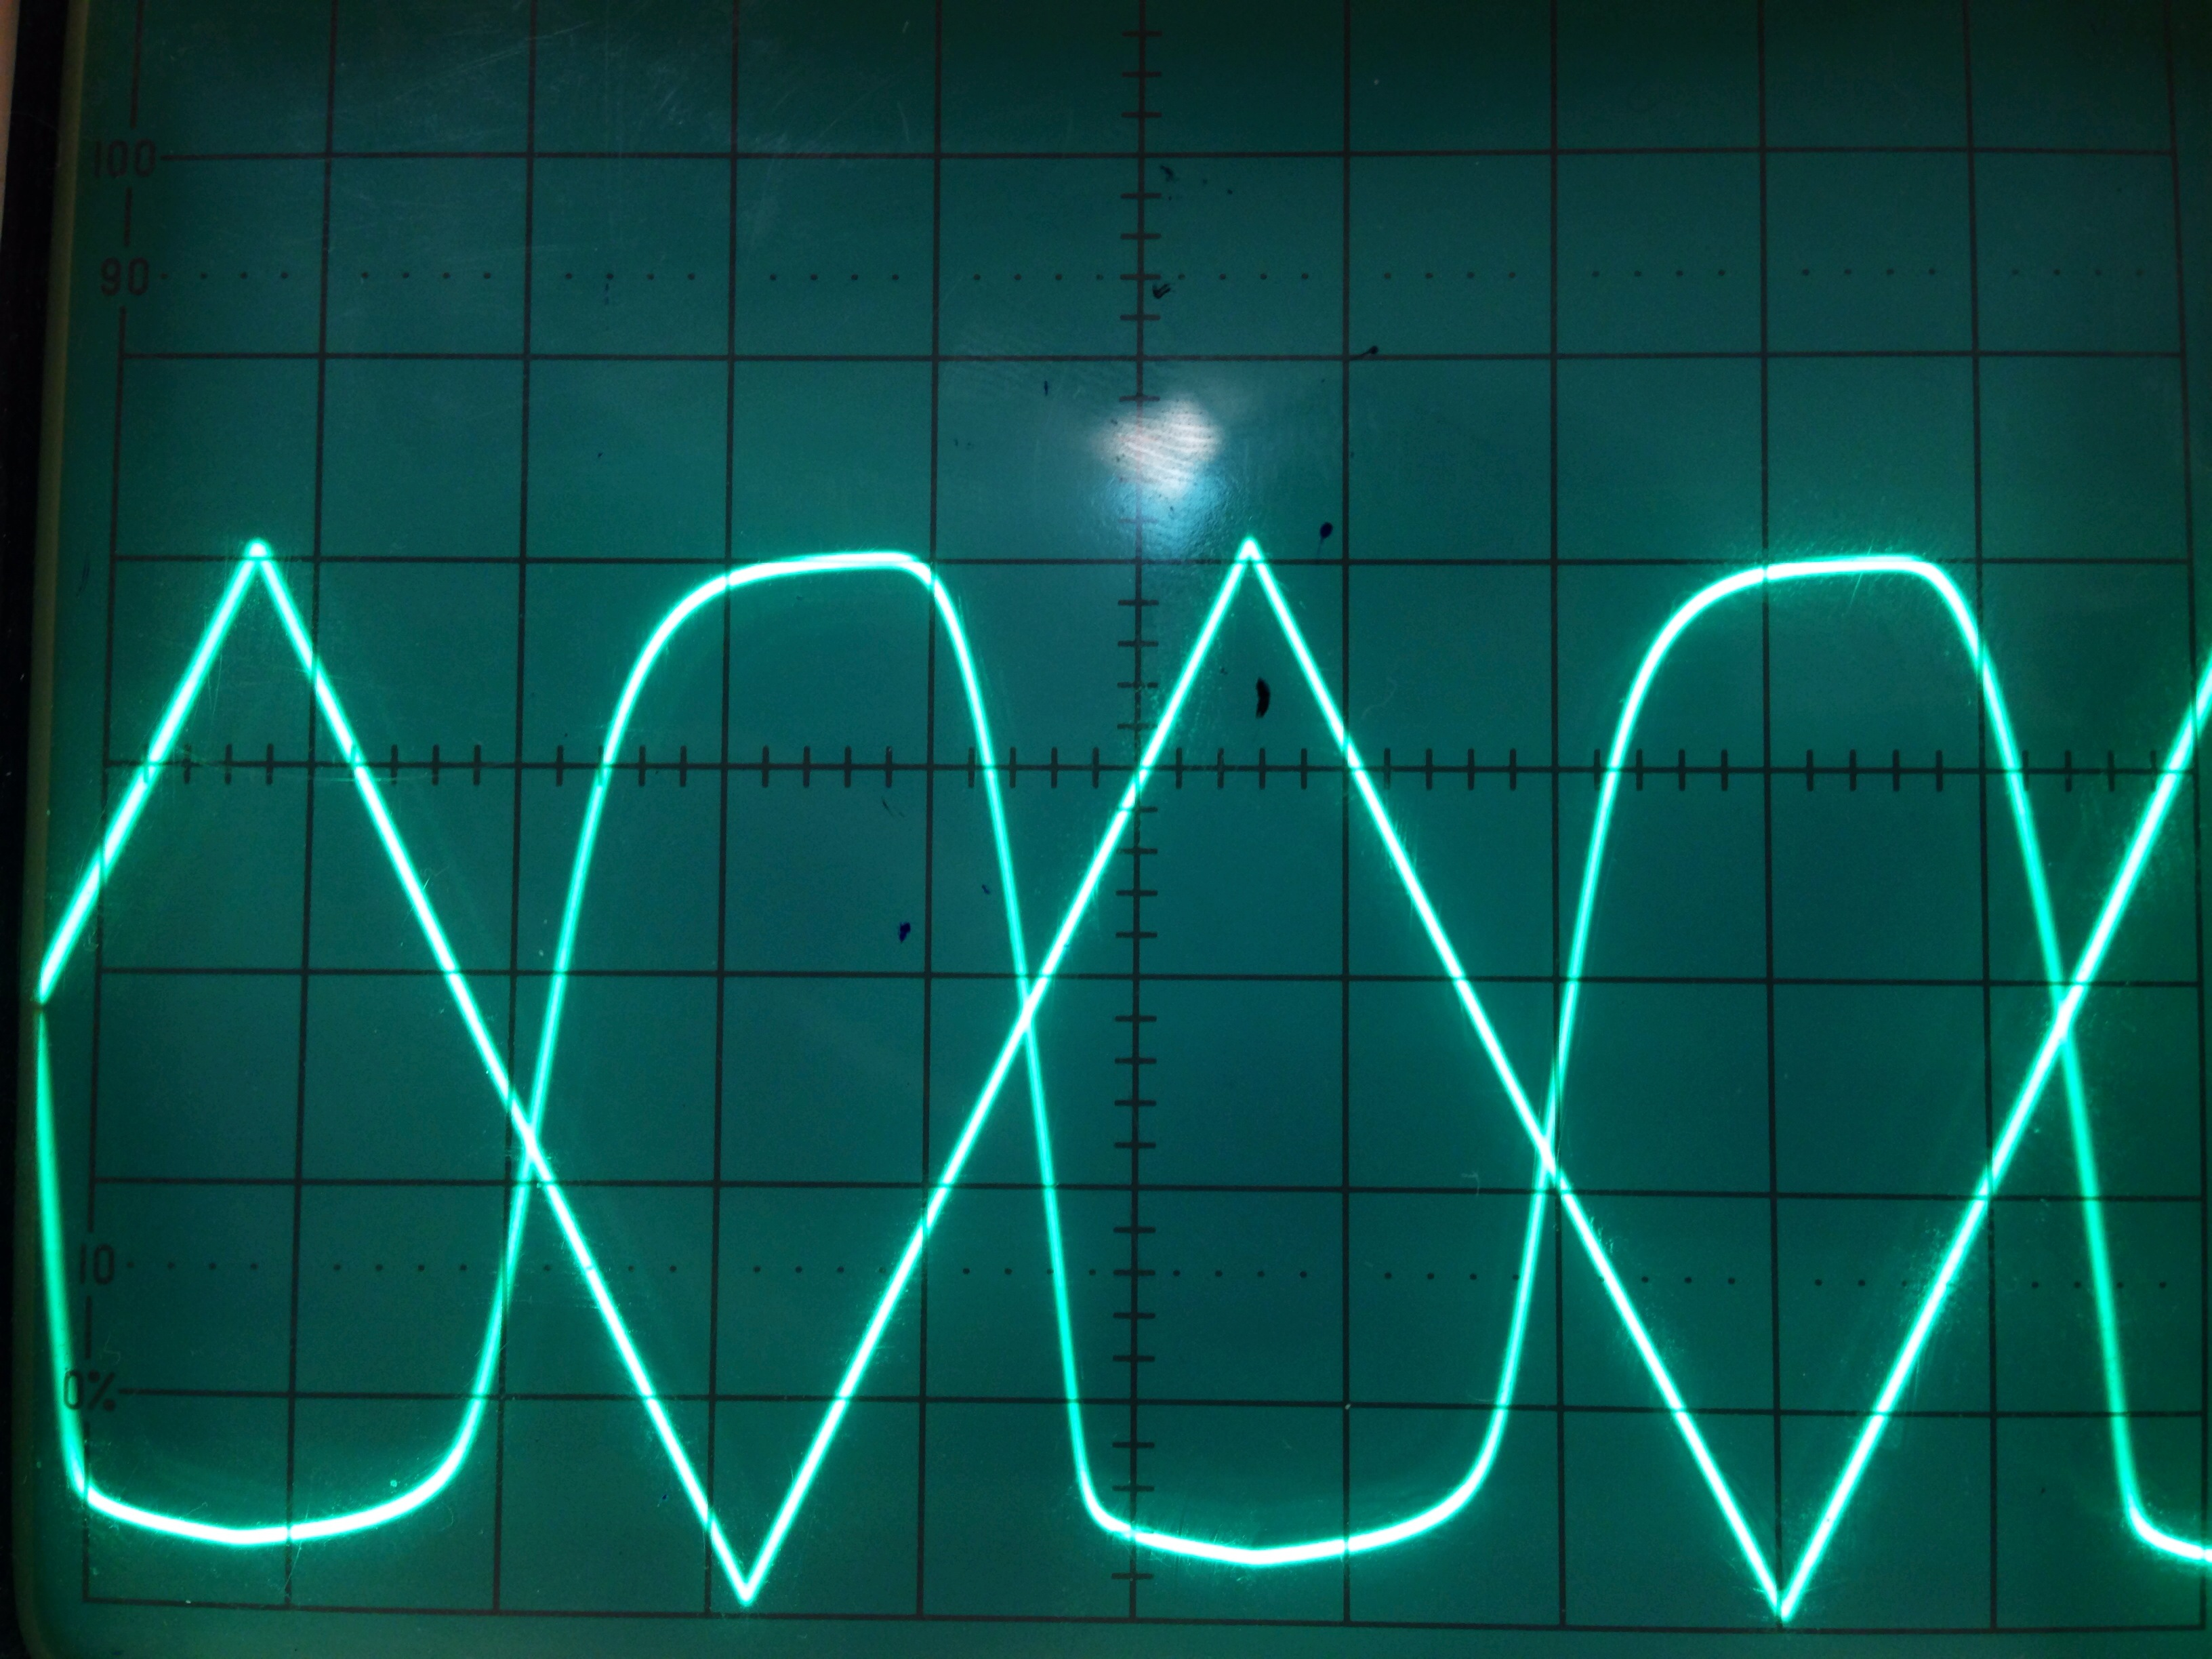
\includegraphics[width=0.8\textwidth]{Imagens/nmos_condensador_grafico.jpg}}}
  \caption{\\Gráfico NMOS com condensador \\Vertical: 1V/div ; \\Horizontal: 0,2ms/div (Time A) }\label{fig:nmos}
\endminipage\hfill
\end{figure}
\begin{figure}[!htb]
\minipage{0.5\textwidth}
  \centerline{\fbox{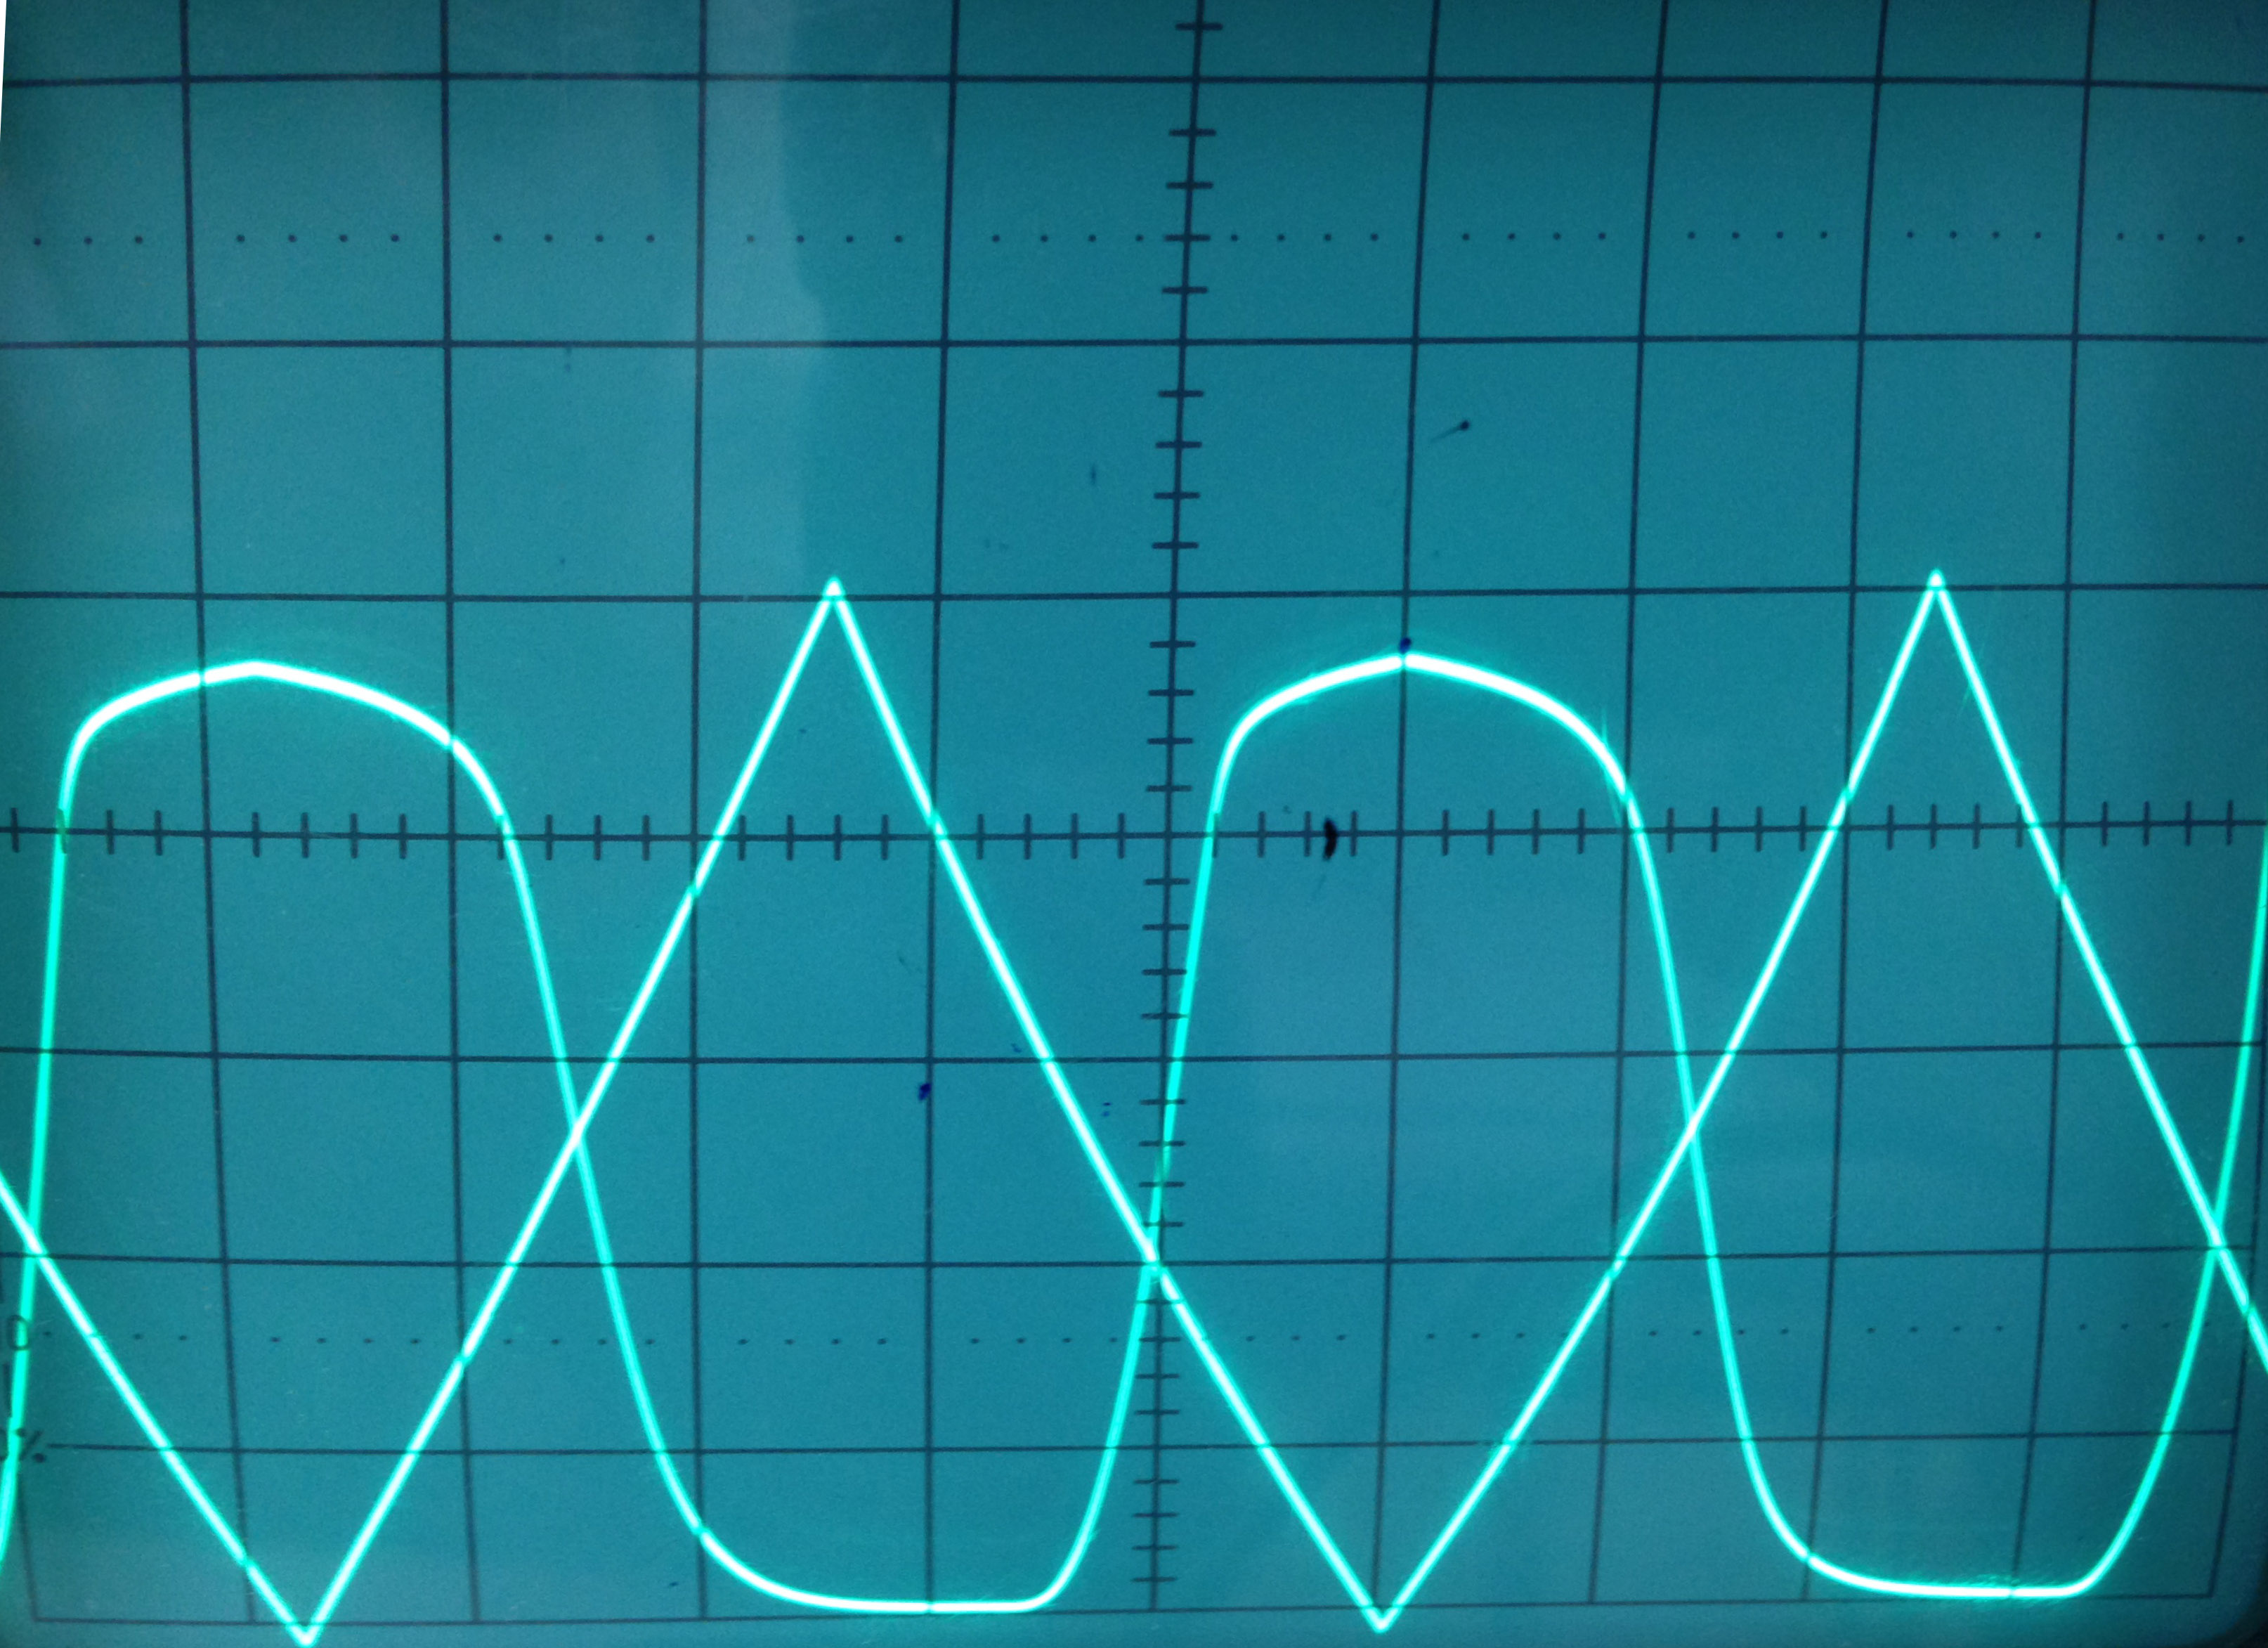
\includegraphics[width=0.8\textwidth]{./Imagens/pmos_grafico_condensador.jpg}}}
  \caption{\\Gráfico PMOS com condensador \\Vertical: 1V/div (ambos); \\Horizontal: 0,2ms/div (Time A)}\label{bjt}
\endminipage\hfill
\minipage{0.5\textwidth}
  \centerline{\fbox{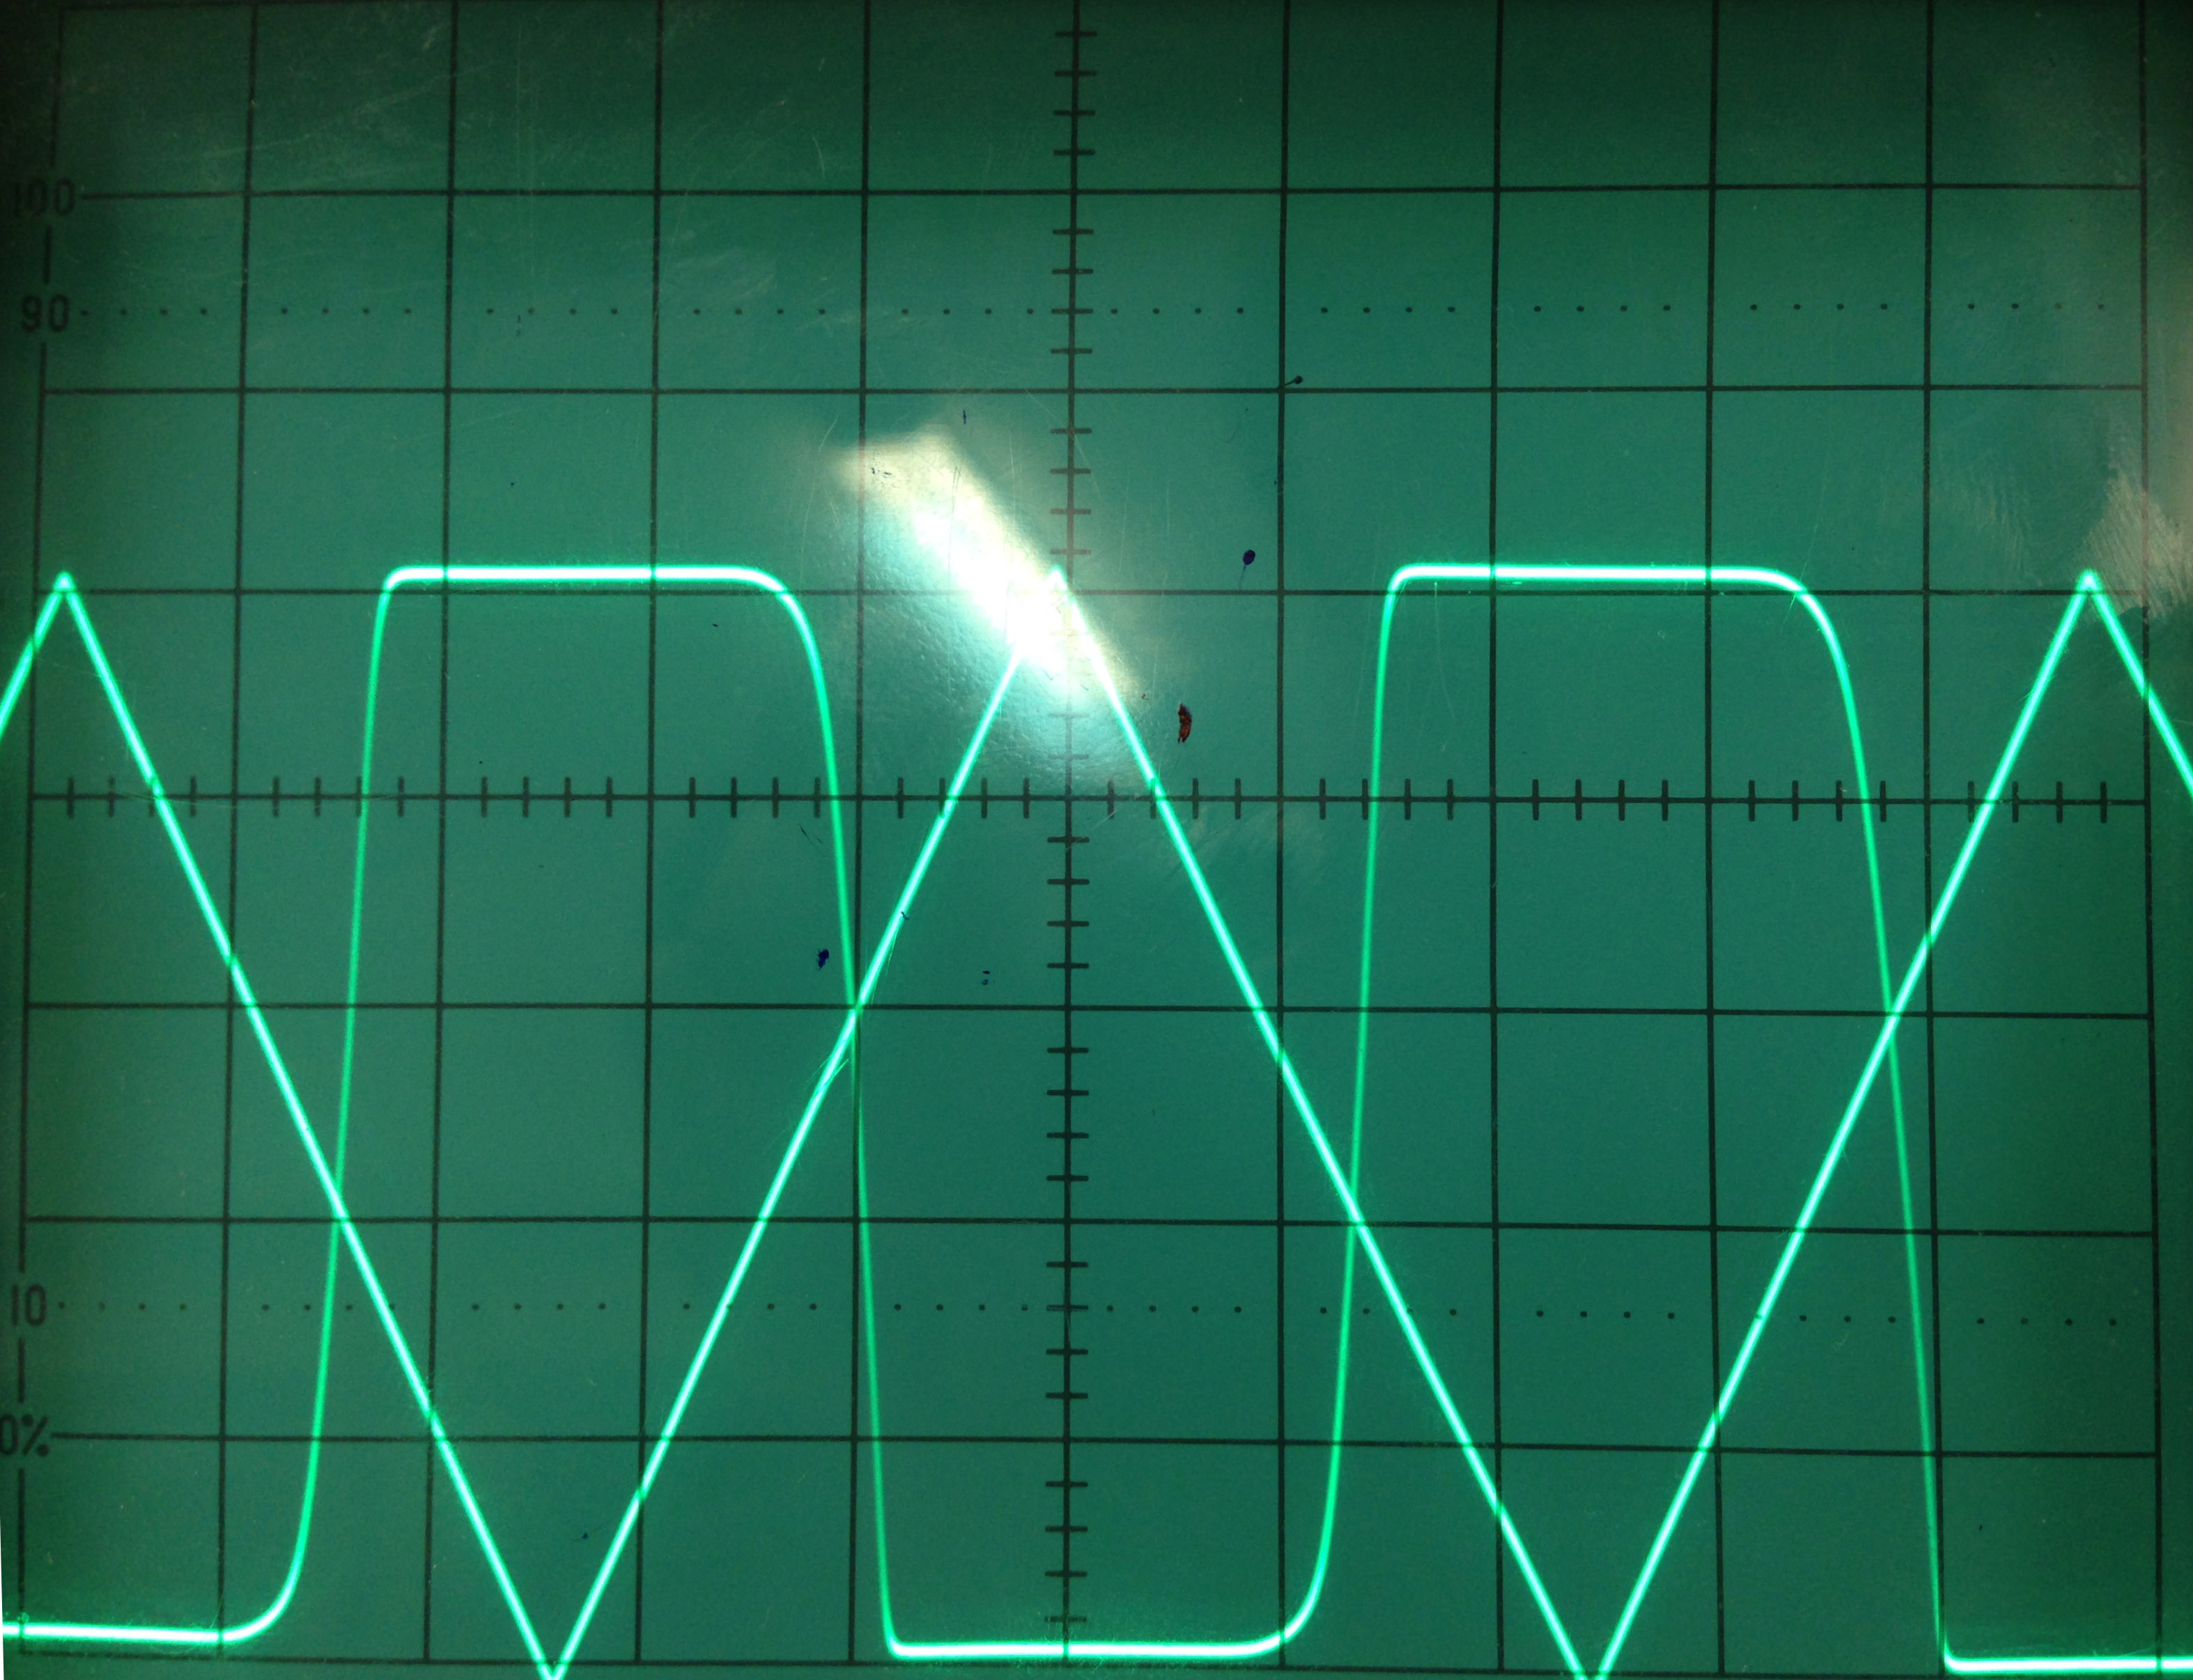
\includegraphics[width=0.8\textwidth]{Imagens/cmos_com_condensador_grafico.jpg}}}
  \caption{\\Gráfico CMOS com condensador \\Vertical: 1V/div (ambos); \\Horizontal: 0,2ms/div (Time A) }\label{fig:nmos}
\endminipage\hfill
\end{figure}

\newpage
BJT:
$t_{sd} = \frac{t_{pHL}+t_{pLH}}{2} = 0,1 ms$
\newline\newline
NMOS:
$t_{sd} = \frac{t_{pHL}+t_{pLH}}{2} = 0,18 ms$
\newline\newline
PMOS:
$t_{sd} = \frac{t_{pHL}+t_{pLH}}{2} = 0,2 ms$
\newline\newline
CMOS:
$t_{sd} = \frac{t_{pHL}+t_{pLH}}{2} = 0,06 ms$
\vspace{0.4cm}

Conclui-se com isto que a porta mais rápida é a CMOS, pois é a que apresenta um menor tempo de subida e descida, isto é, o tempo que demora a mudar de nível lógico.

\section{Parte III - Aplicações	de	Circuitos	Lógicos	CMOS}
\begin{figure}[h]
  \centerline{\fbox{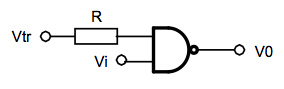
\includegraphics[width=0.3\textwidth]{./Imagens/parte3circuito1.jpg}}}
  \caption{$V_{tr}$ = $V_{DD}$ e R = 1k$\Omega$}\label{cmos}
\end{figure}

\subsection{Tabela de verdade de um NAND}

\begin{table}[h]
\centerline{
\begin{tabular}{|l|l|l|}
\hline
$V_{tr}$ & $V_{i}$ & $V_{0}$ \\ \hline
0 & 0 & 1 \\ \hline
0 & 1 & 1 \\ \hline
1 & 0 & 1 \\ \hline
1 & 1 & 0 \\ \hline
\end{tabular}}
\caption{\\Tabela de verdade de um NAND \\implementado pelo circuito}\label{fig:fig_diodo}
\end{table}

\subsection{Valores de $V_{iH}$ e de $V_{iL}$}
\begin{figure}[h]
  \centerline{\fbox{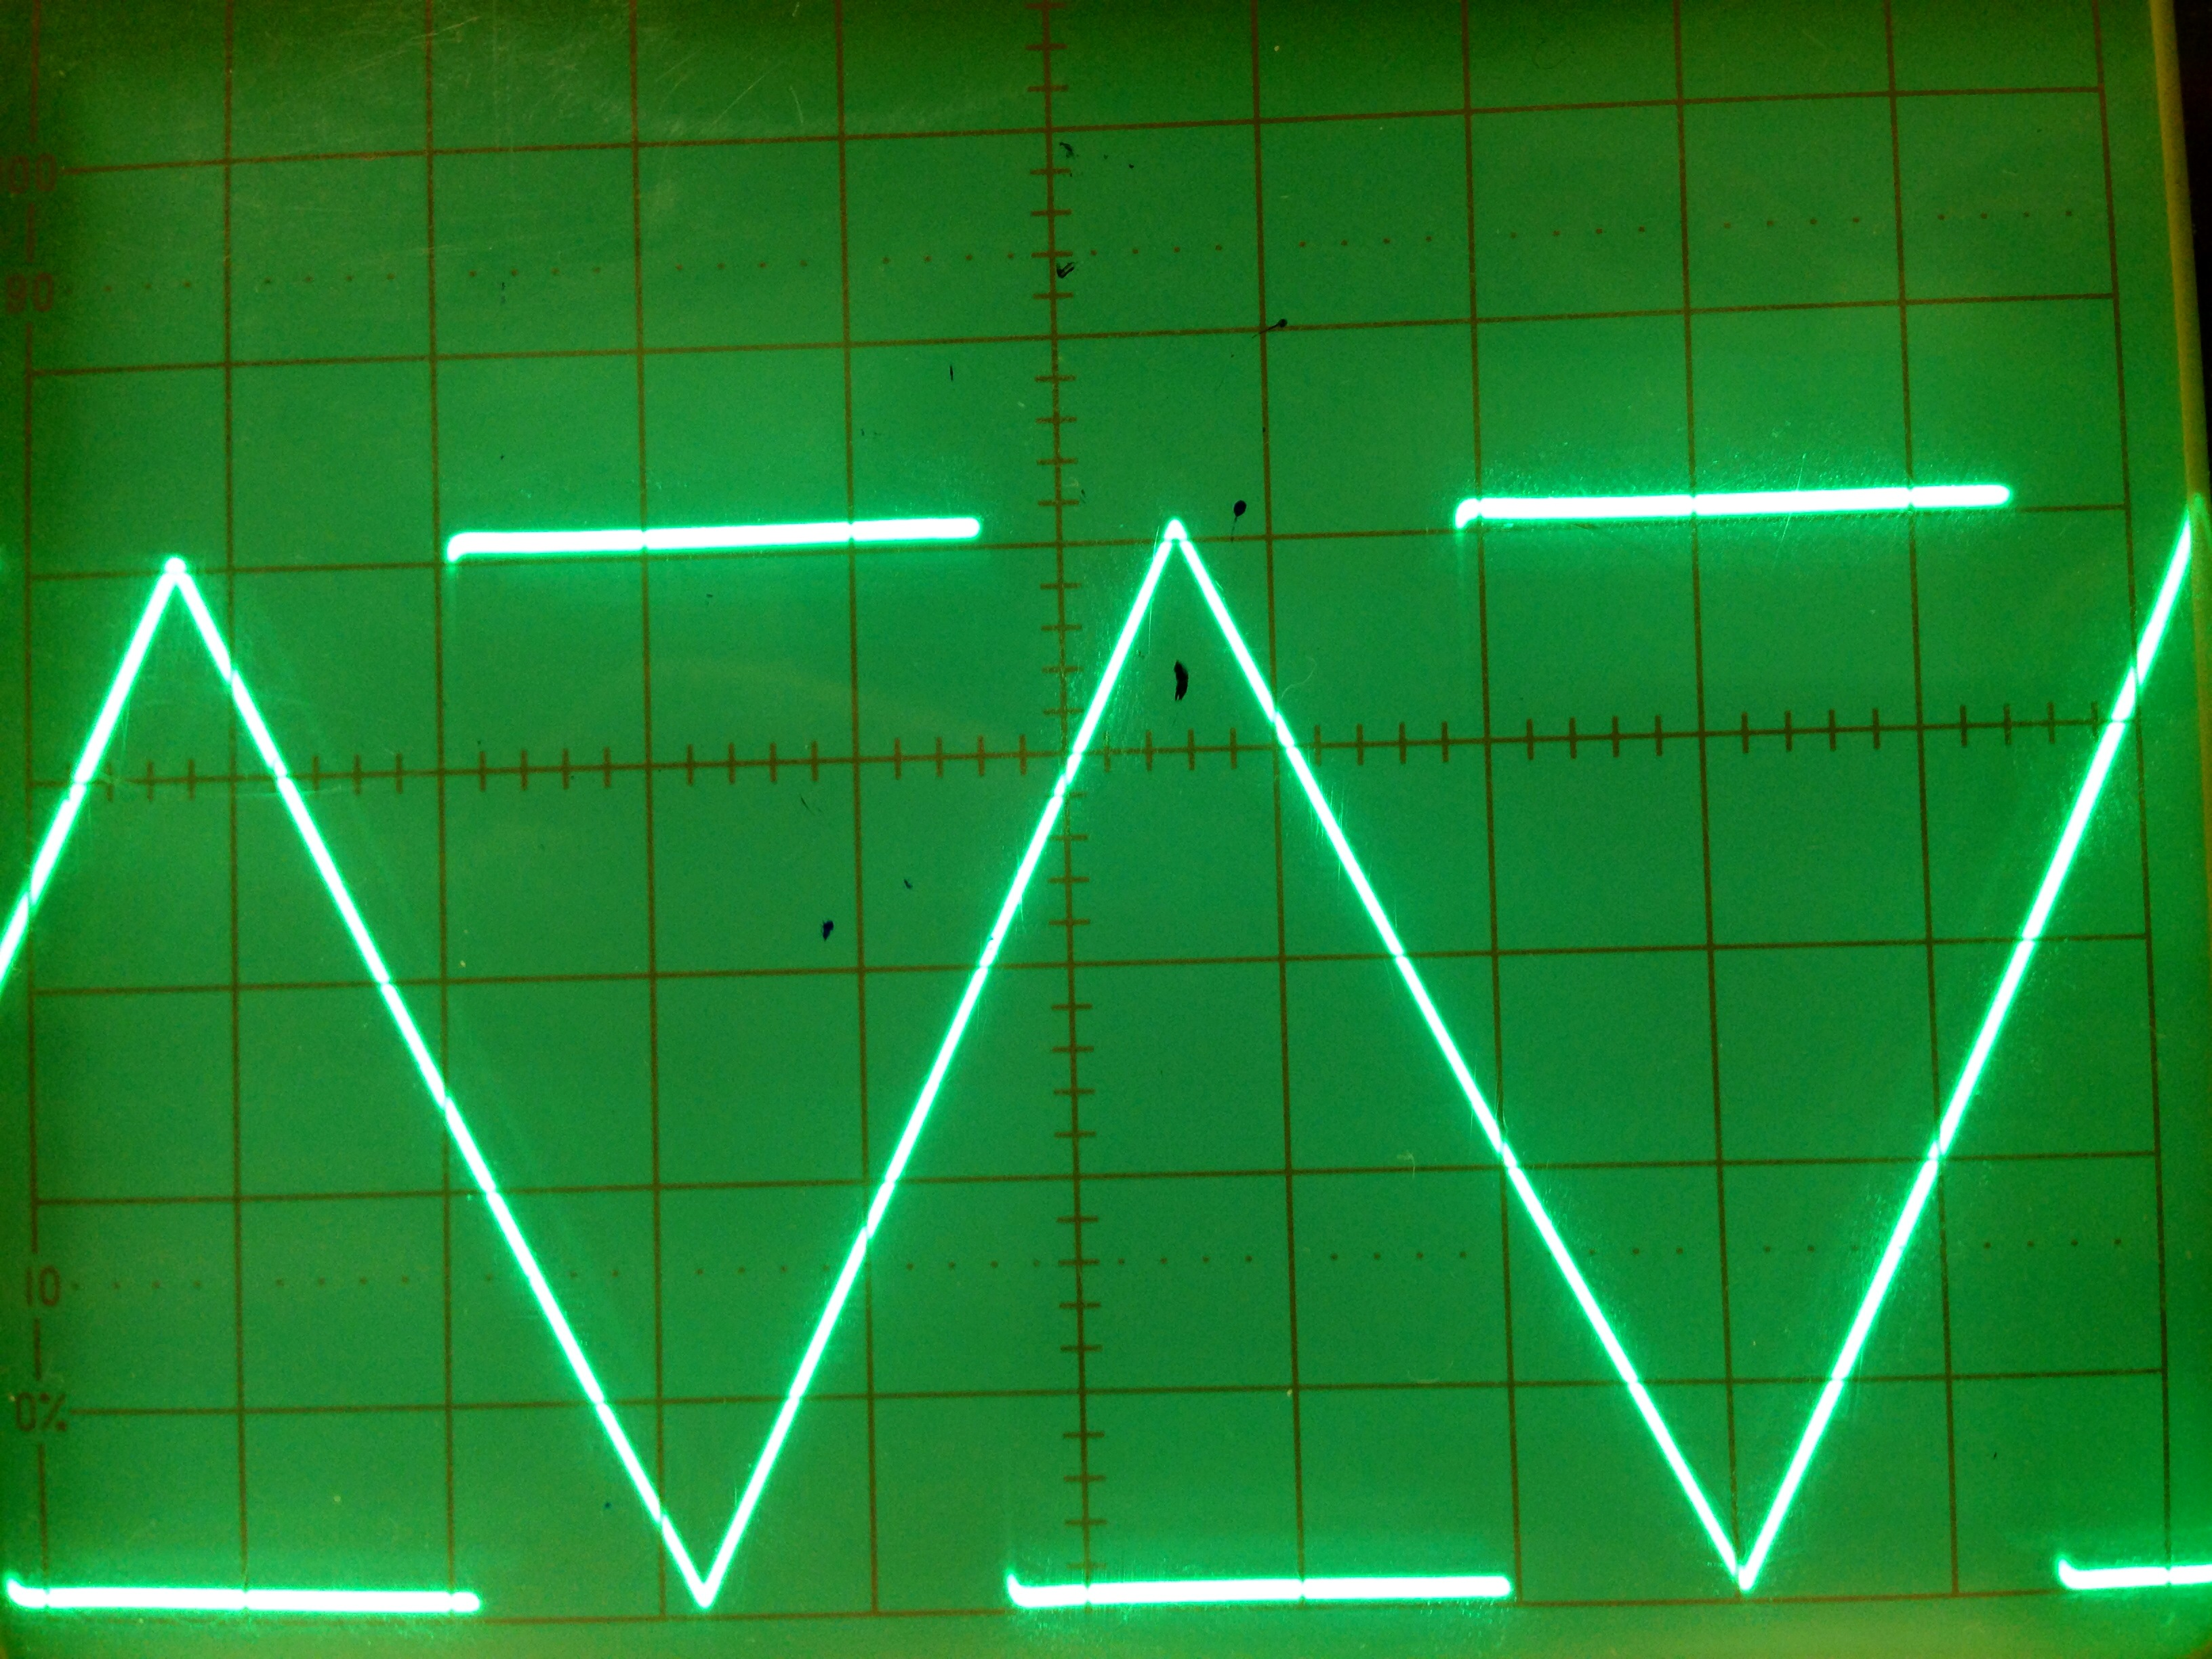
\includegraphics[width=0.5\textwidth]{./Imagens/parte3_ex1_grafico.jpg}}}
  \caption{Vertical: 1V/div (ambos); \\Horizontal: 0,2ms/div (Time A)}\label{cmos}
\end{figure}

Valor de $V_{iH}$, quando o sinal triangular sobe o $V_0$ passa de 1 para 0, aos 3,2V e de $V_{iL}$, quando o sinal triangular desce o $V_0$ passa de 0 para 1 aos 2V.

\newpage
\begin{figure}[h]
  \centerline{\fbox{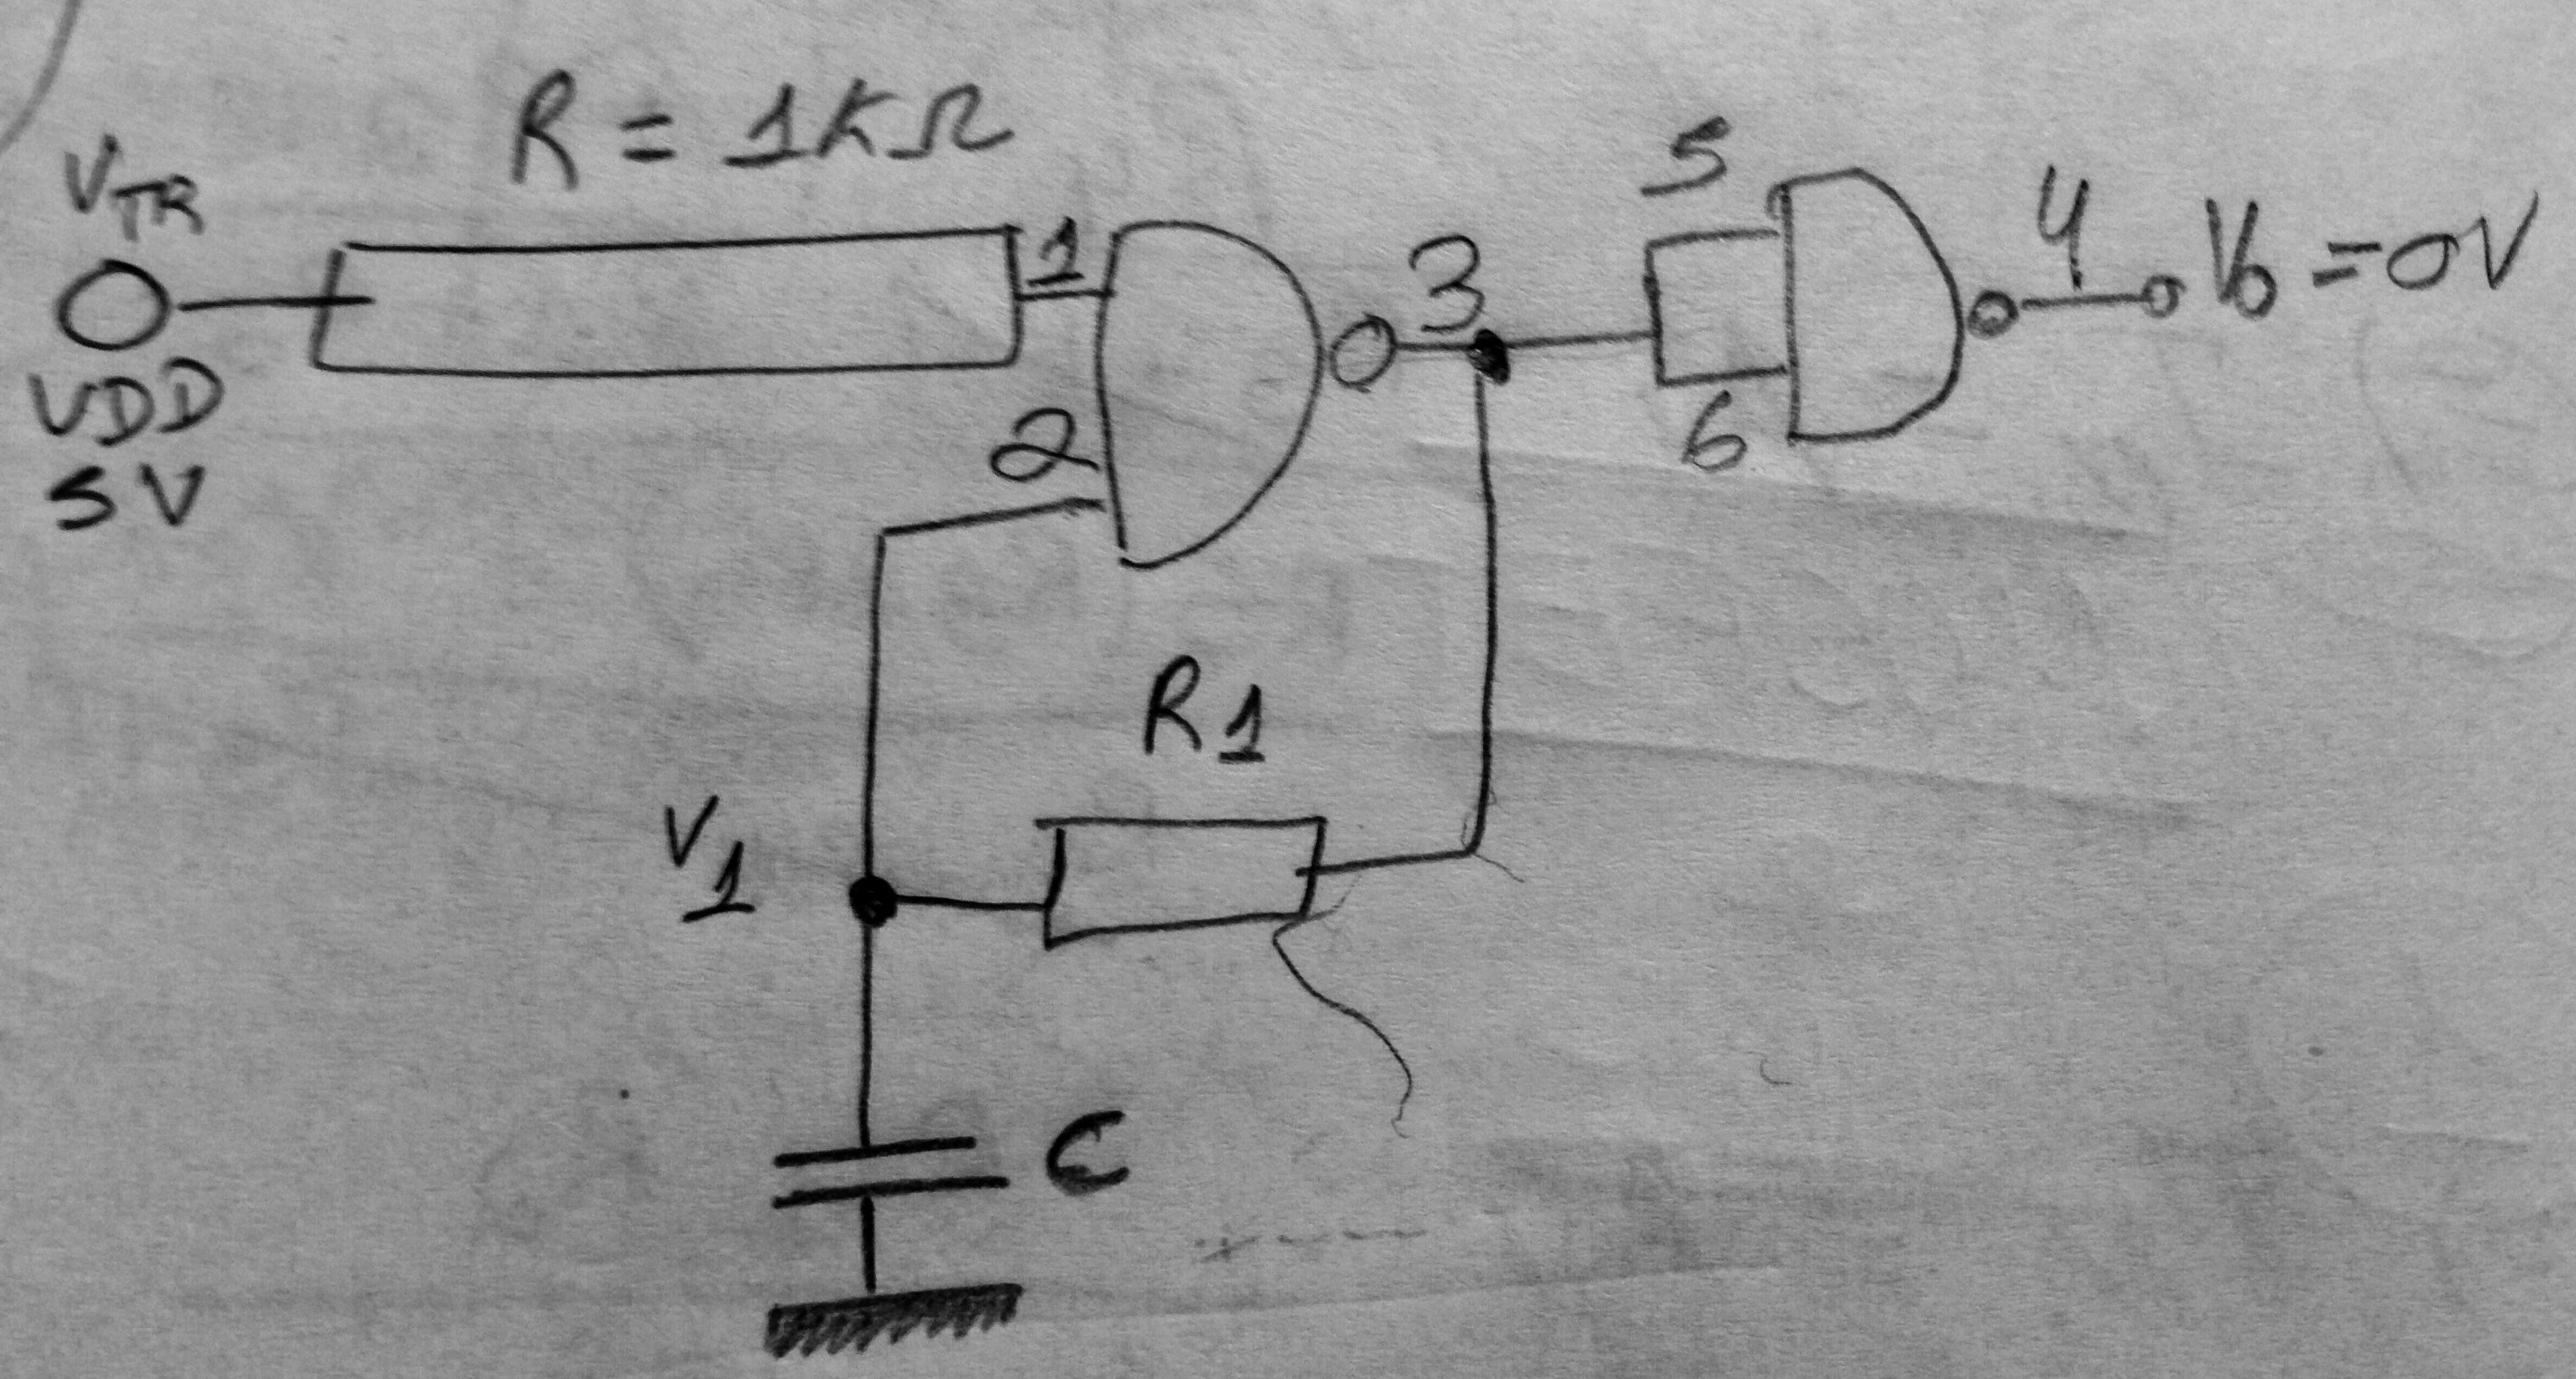
\includegraphics[width=0.5\textwidth]{./Imagens/parte3circuito2.jpg}}}
  \caption{$V_{tr}$=$V_{DD}$, R=1k$\Omega$, $R_1$=100k$\Omega$ e C=10nF}\label{cmos}
\end{figure}

\subsection{Verificar que o circuito funciona como gerador de onda rectangular}

\begin{figure}[h]
  \centerline{\fbox{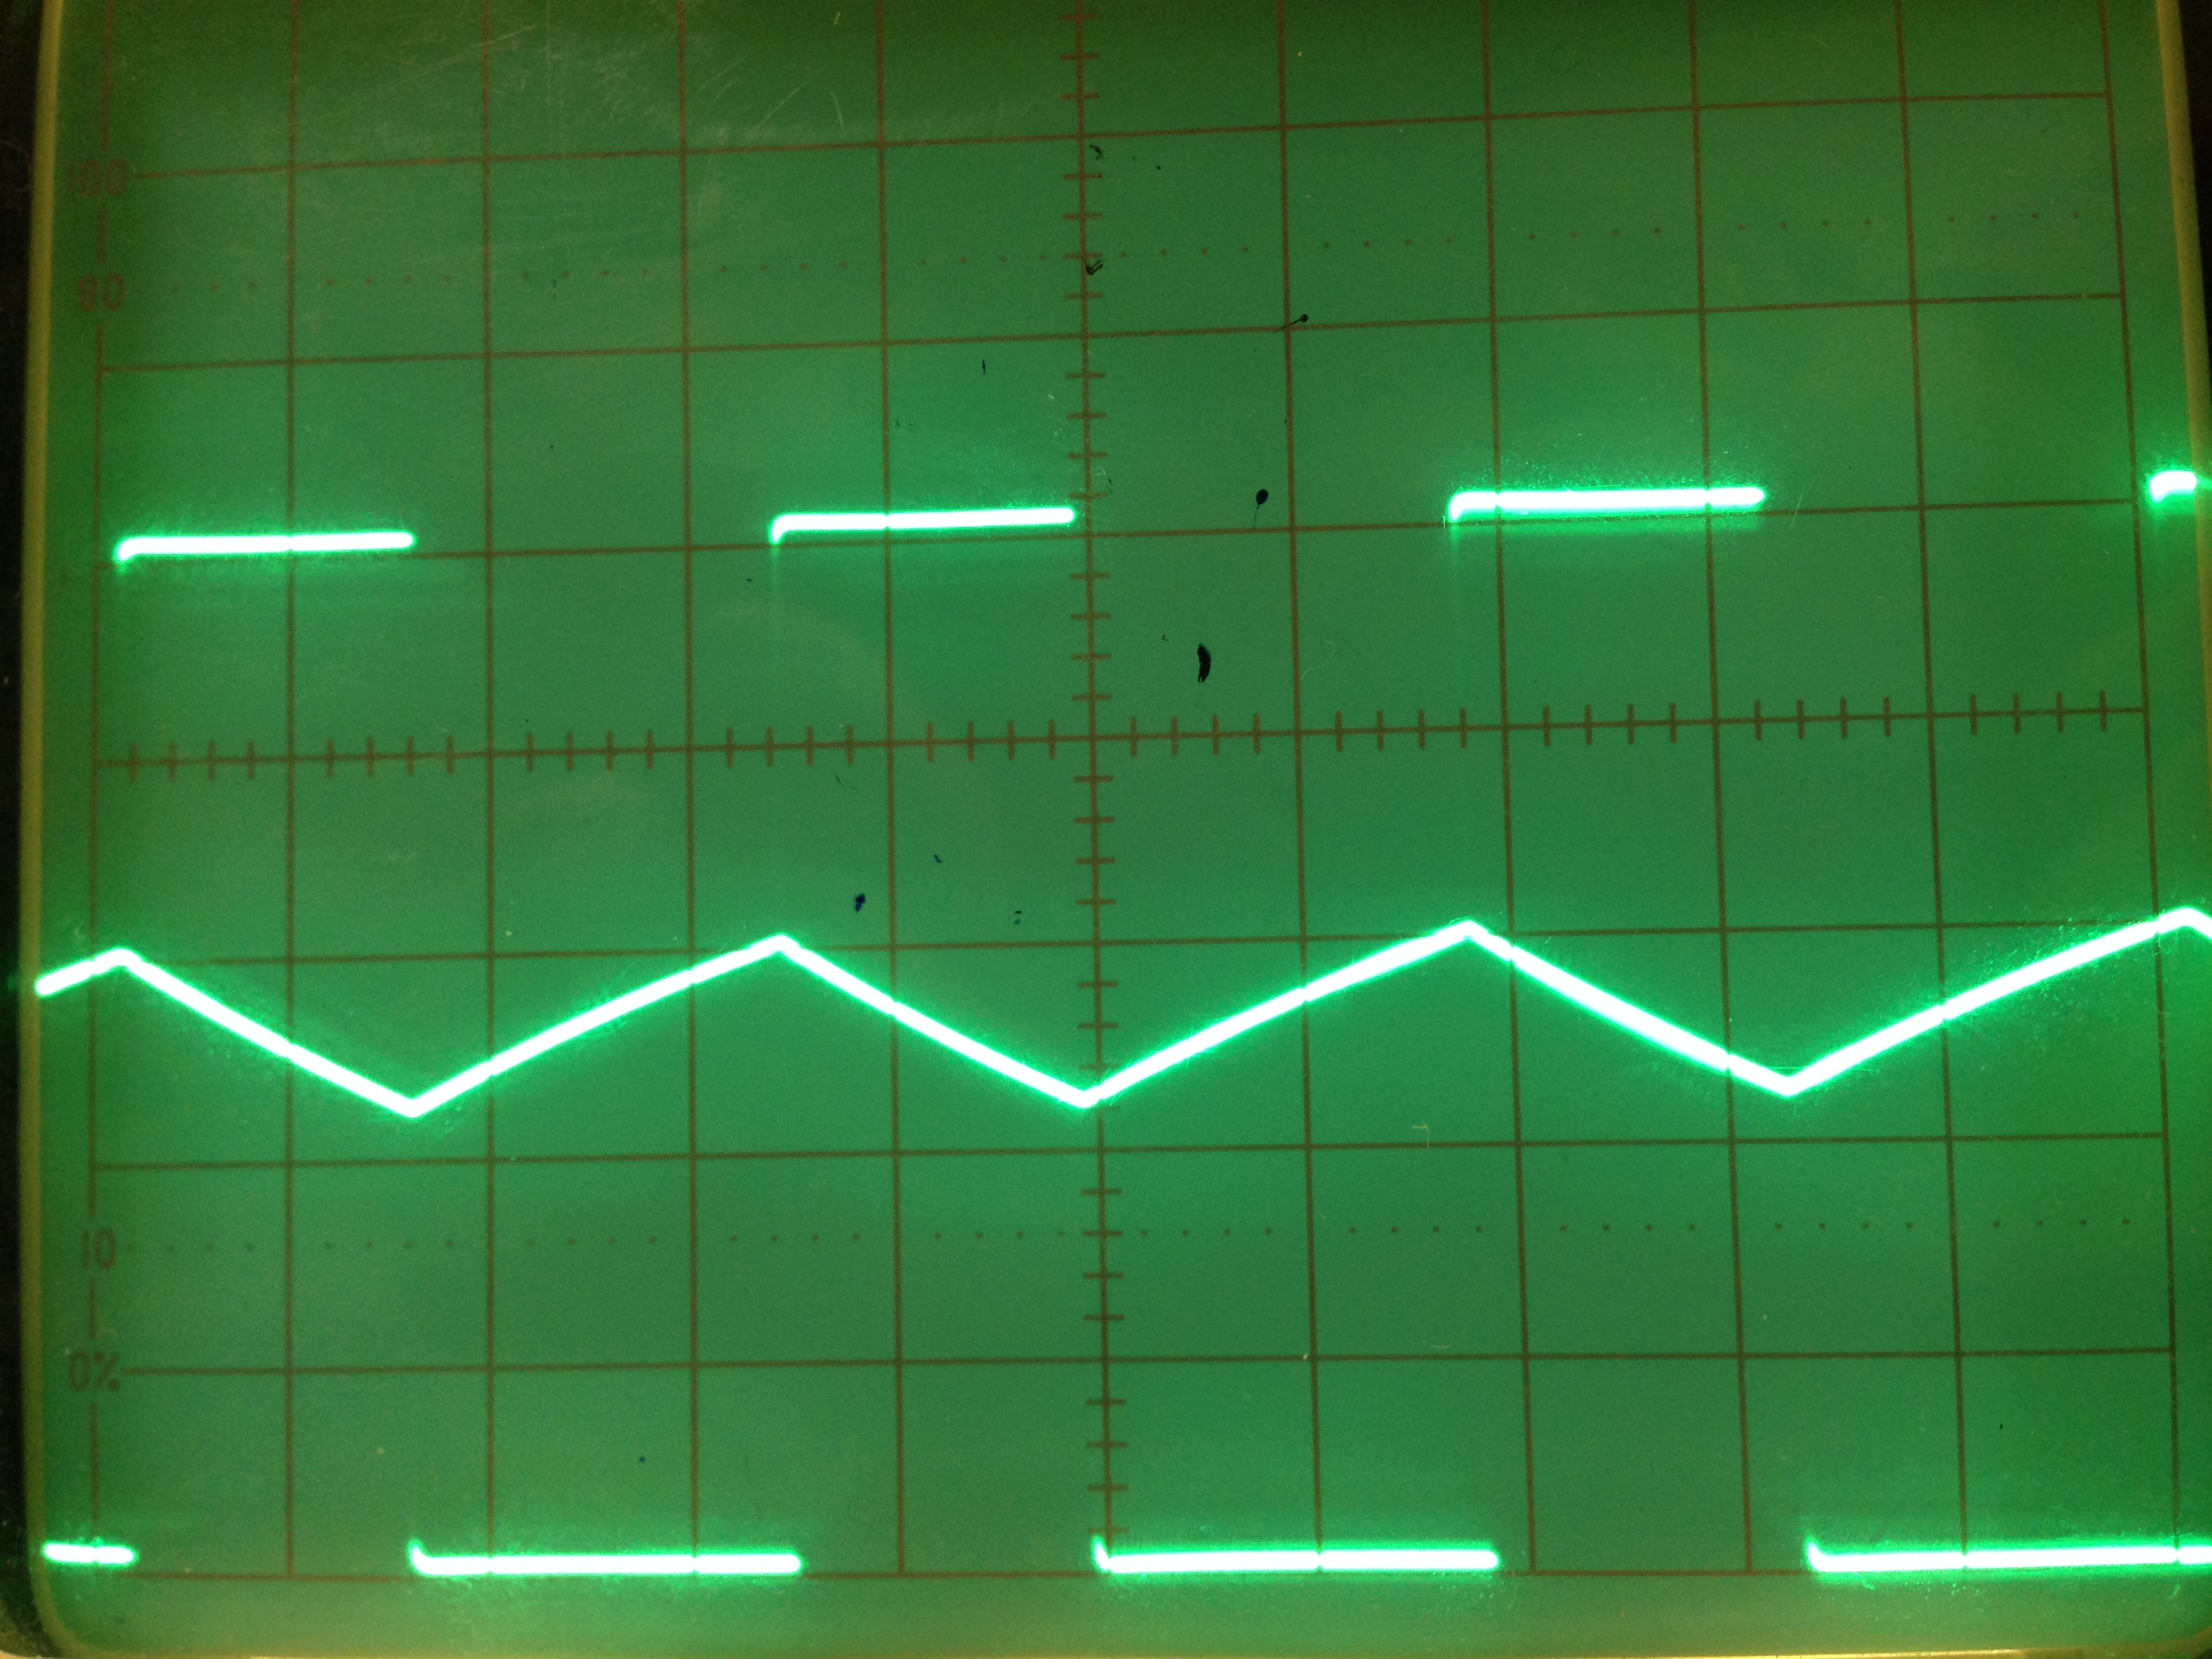
\includegraphics[width=0.4\textwidth]{./Imagens/parte3exercicio3_grafico.jpg}}}
  \caption{Vertical: 1V/div (ambos); \\Horizontal: 0,2ms/div (Time A)}\label{cmos}
\end{figure}

\subsection{Comparar a amplitude do sinal de $V_1$ com $V_{iH}$ e de $V_{iL}$}

Amplitude de $V_1$ = 0,8V = 3,0 - 2,2V

Quando a saída do primeiro NAND é 5V (valor lógico 1) o condensador carrega e o inverso acontece quando o condesador descarrega ficando assim a saída do segundo NAND a 5V (valor lógico 1).

\begin{table}[h]
\centerline{
\begin{tabular}{|l|l|l|}
\hline
$V_{rt}$ & $V_{1}$ & $V_{0} = \neg(\neg(V_{rt}*V_{1})*\neg(V{rt}*V{1}))$ \\ \hline
5 & 0 & 0 $\Rightarrow$ condensador descarrega\\ \hline
5 & 5 & 1 $\Rightarrow$ condensador carrega\\ \hline
\end{tabular}}
\caption{}\label{fig:fig_diodo}
\end{table}

$V_1$ comporta-se como a saída de um circuito RC passa-baixo porque permite a passagem de baixas frequências sem dificuldades e atenua a amplitude das frequências maiores que a frequência de corte.
\vspace{0.5cm}

\subsection{Calcular para $V_0$ o $t_{on}$, T e duty cycle ($\delta$). Explicar porquê que $\delta$ $\neq$ 50\%}

$t_{on} = 1,5V$ e $T = 3,4V$ então:
\vspace{0.3cm}

$\delta = \frac{t_{on}}{T}\times100 = \frac{1,5}{3,4}\times100 \simeq 44 \% $
\vspace{0.3cm}

É $\neq$ de 50\% porque o condensador demora mais tempo a carregar do que a descarregar, estando menos tempo a 1 do que a 0.

\subsection{Gerador de “bursts”}
\begin{figure}[h]
  \centerline{\fbox{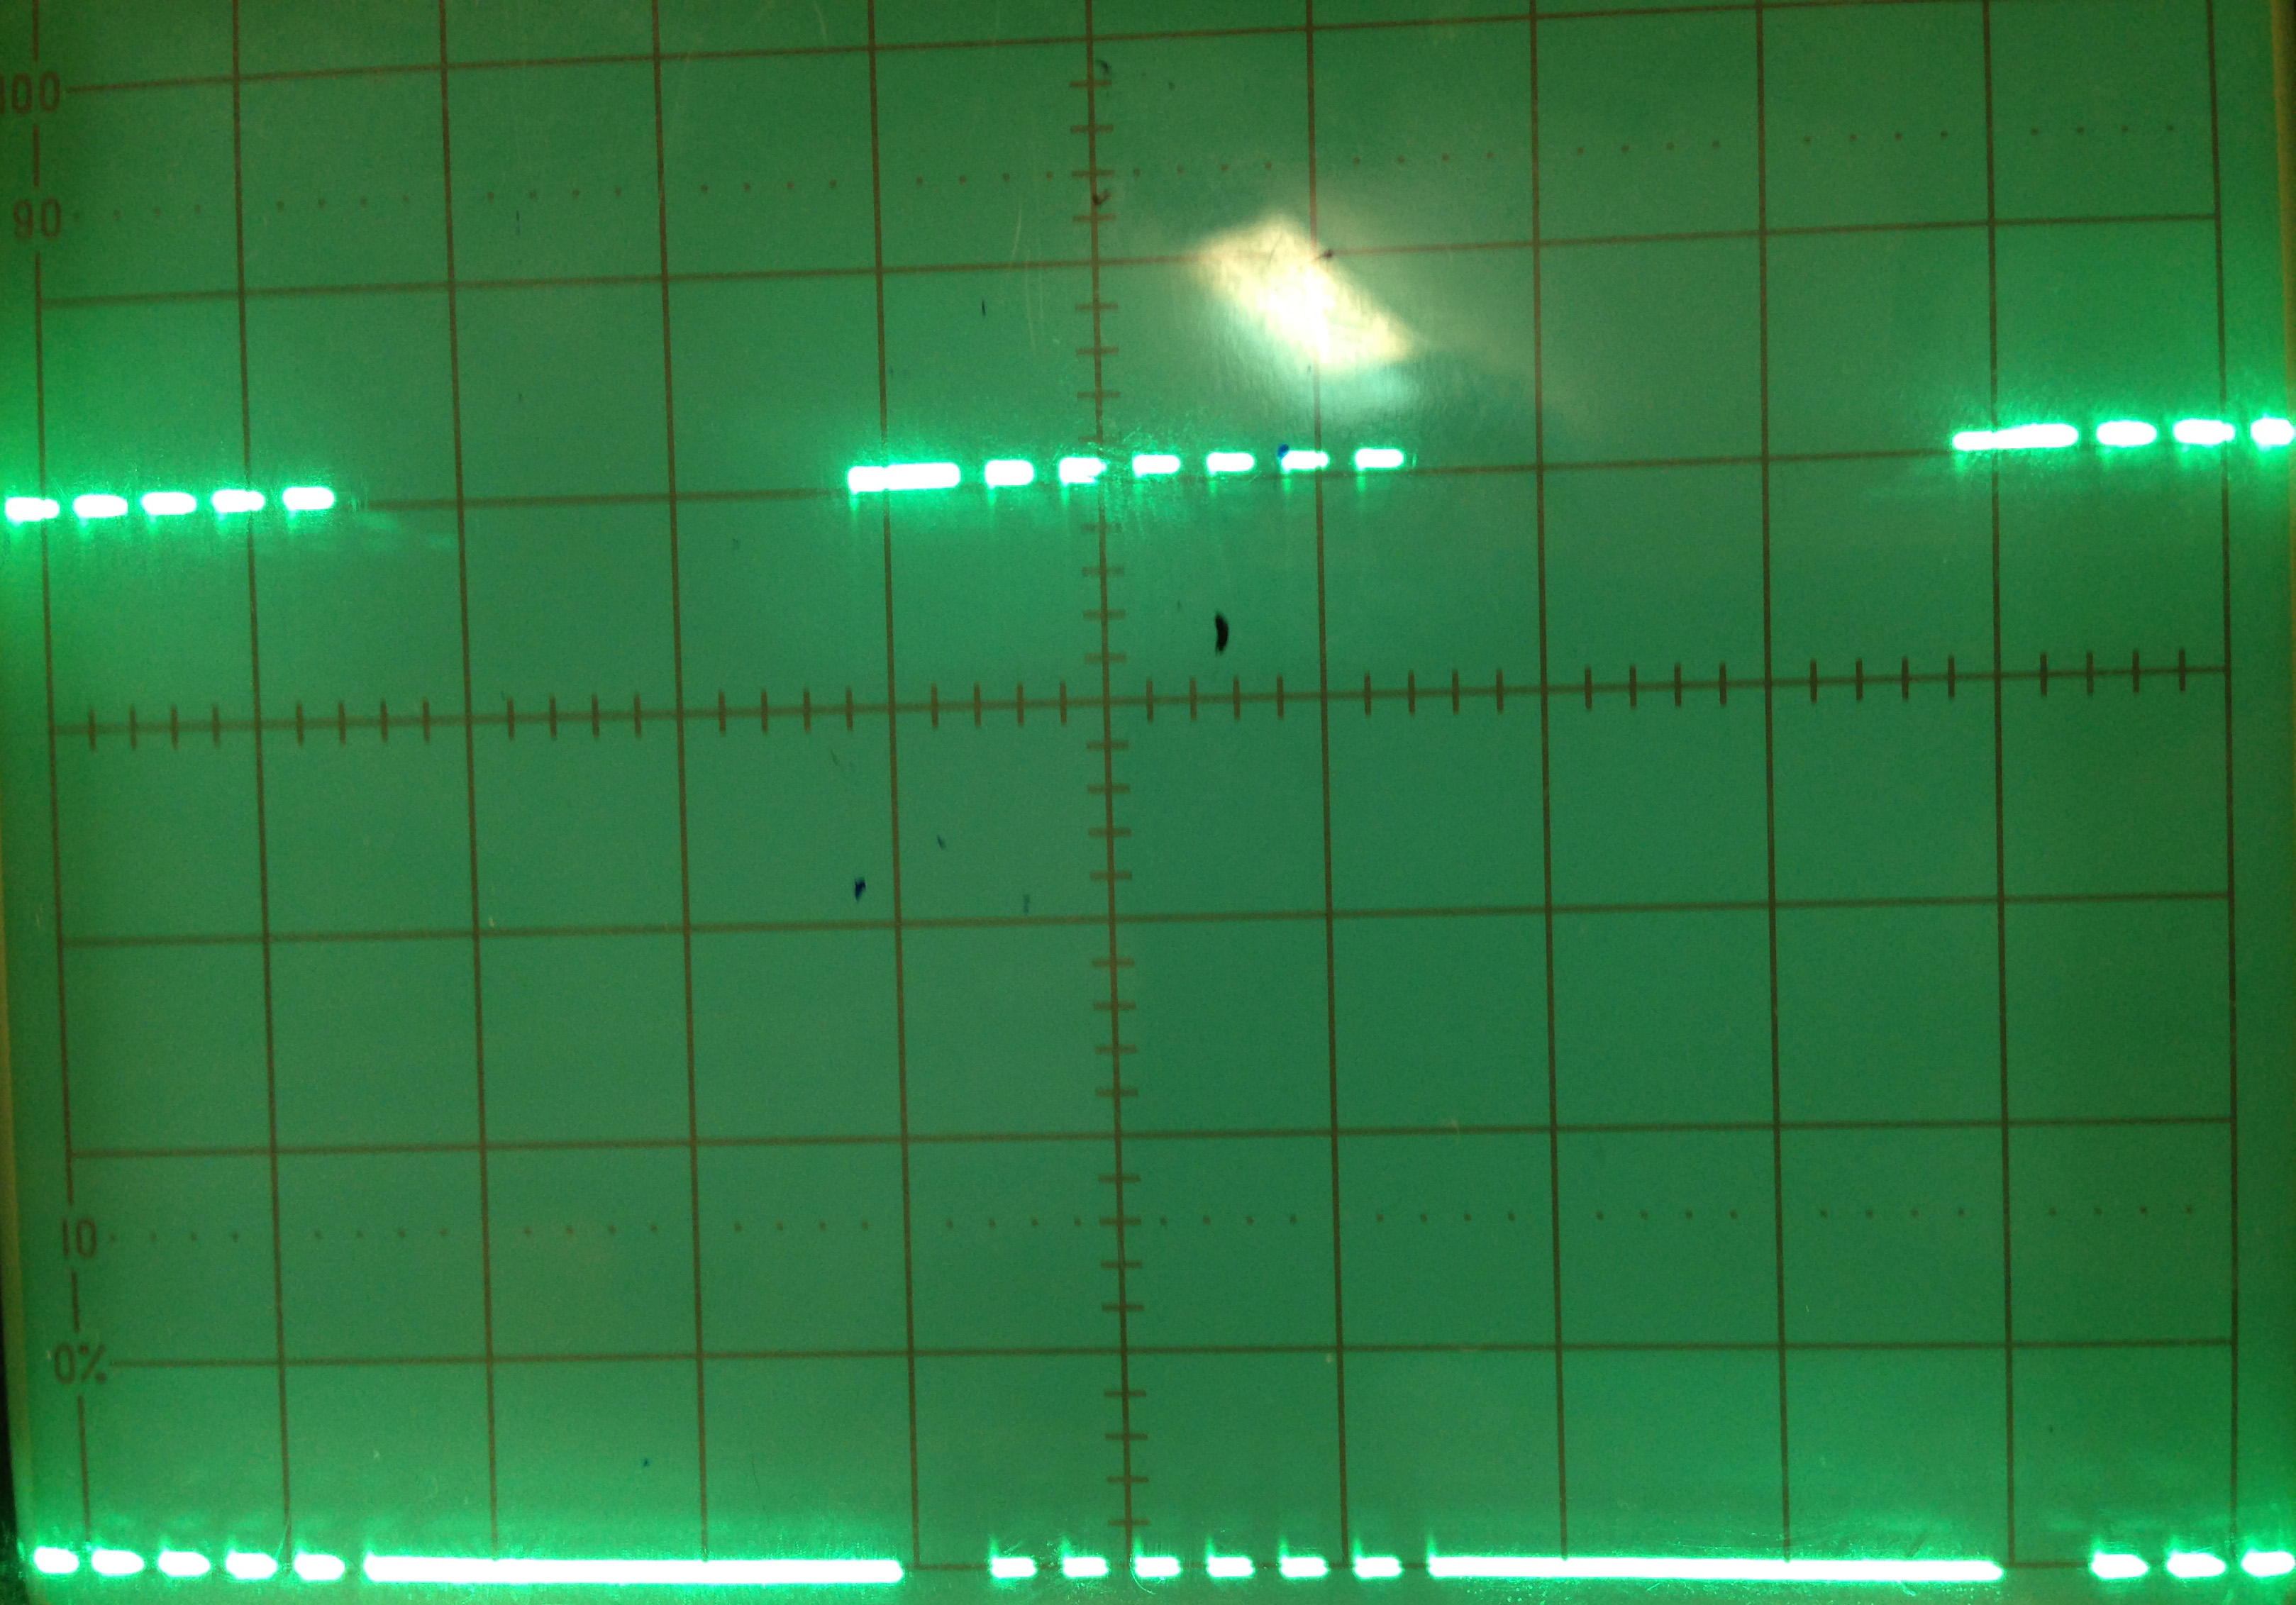
\includegraphics[width=0.4\textwidth]{./Imagens/parte3exercicio6.jpg}}}
  \caption{Vertical: 1V/div (ambos); \\Horizontal: 0,2ms/div (Time A)}\label{cmos}
\end{figure}

Obtivémos um gerador de bursts. Quando o sinal vai a 1 a saída toma o valor don't care.

\end{document}